\documentclass[twoside]{book}

% Packages required by doxygen
\usepackage{calc}
\usepackage{doxygen}
\usepackage{graphicx}
\usepackage[utf8]{inputenc}
\usepackage{makeidx}
\usepackage{multicol}
\usepackage{multirow}
\usepackage{textcomp}
\usepackage[table]{xcolor}

% Font selection
\usepackage[T1]{fontenc}
\usepackage{mathptmx}
\usepackage[scaled=.90]{helvet}
\usepackage{courier}
\usepackage{amssymb}
\usepackage{sectsty}
\renewcommand{\familydefault}{\sfdefault}
\allsectionsfont{%
  \fontseries{bc}\selectfont%
  \color{darkgray}%
}
\renewcommand{\DoxyLabelFont}{%
  \fontseries{bc}\selectfont%
  \color{darkgray}%
}

% Page & text layout
\usepackage{geometry}
\geometry{%
  a4paper,%
  top=2.5cm,%
  bottom=2.5cm,%
  left=2.5cm,%
  right=2.5cm%
}
\tolerance=750
\hfuzz=15pt
\hbadness=750
\setlength{\emergencystretch}{15pt}
\setlength{\parindent}{0cm}
\setlength{\parskip}{0.2cm}
\makeatletter
\renewcommand{\paragraph}{%
  \@startsection{paragraph}{4}{0ex}{-1.0ex}{1.0ex}{%
    \normalfont\normalsize\bfseries\SS@parafont%
  }%
}
\renewcommand{\subparagraph}{%
  \@startsection{subparagraph}{5}{0ex}{-1.0ex}{1.0ex}{%
    \normalfont\normalsize\bfseries\SS@subparafont%
  }%
}
\makeatother

% Headers & footers
\usepackage{fancyhdr}
\pagestyle{fancyplain}
\fancyhead[LE]{\fancyplain{}{\bfseries\thepage}}
\fancyhead[CE]{\fancyplain{}{}}
\fancyhead[RE]{\fancyplain{}{\bfseries\leftmark}}
\fancyhead[LO]{\fancyplain{}{\bfseries\rightmark}}
\fancyhead[CO]{\fancyplain{}{}}
\fancyhead[RO]{\fancyplain{}{\bfseries\thepage}}
\fancyfoot[LE]{\fancyplain{}{}}
\fancyfoot[CE]{\fancyplain{}{}}
\fancyfoot[RE]{\fancyplain{}{\bfseries\scriptsize Generated on Tue Feb 4 2014 21\-:08\-:09 for Senergy by Doxygen }}
\fancyfoot[LO]{\fancyplain{}{\bfseries\scriptsize Generated on Tue Feb 4 2014 21\-:08\-:09 for Senergy by Doxygen }}
\fancyfoot[CO]{\fancyplain{}{}}
\fancyfoot[RO]{\fancyplain{}{}}
\renewcommand{\footrulewidth}{0.4pt}
\renewcommand{\chaptermark}[1]{%
  \markboth{#1}{}%
}
\renewcommand{\sectionmark}[1]{%
  \markright{\thesection\ #1}%
}

% Indices & bibliography
\usepackage{natbib}
\usepackage[titles]{tocloft}
\setcounter{tocdepth}{3}
\setcounter{secnumdepth}{5}
\makeindex

% Hyperlinks (required, but should be loaded last)
\usepackage{ifpdf}
\ifpdf
  \usepackage[pdftex,pagebackref=true]{hyperref}
\else
  \usepackage[ps2pdf,pagebackref=true]{hyperref}
\fi
\hypersetup{%
  colorlinks=true,%
  linkcolor=blue,%
  citecolor=blue,%
  unicode%
}

% Custom commands
\newcommand{\clearemptydoublepage}{%
  \newpage{\pagestyle{empty}\cleardoublepage}%
}


%===== C O N T E N T S =====

\begin{document}

% Titlepage & ToC
\hypersetup{pageanchor=false}
\pagenumbering{roman}
\begin{titlepage}
\vspace*{7cm}
\begin{center}%
{\Large Senergy \\[1ex]\large 1.\-0 }\\
\vspace*{1cm}
{\large Generated by Doxygen 1.8.6}\\
\vspace*{0.5cm}
{\small Tue Feb 4 2014 21:08:09}\\
\end{center}
\end{titlepage}
\clearemptydoublepage
\tableofcontents
\clearemptydoublepage
\pagenumbering{arabic}
\hypersetup{pageanchor=true}

%--- Begin generated contents ---
\chapter{About Senergy}
\label{index}\hypertarget{index}{}\hyperlink{namespace_senergy}{Senergy} is a open-\/source, recursive D\-N\-S server written in C++. \hyperlink{namespace_senergy}{Senergy} is currently being written for a graduation project, but intends to be light D\-N\-S server, mostly for learning purposes. \hyperlink{namespace_senergy}{Senergy} is developed on Linux (Xubuntu 14.\-04 x64) but could be (with a little work) compiled on other platforms such as Windows or Mac O\-S X. \hyperlink{namespace_senergy}{Senergy} uses Git for source version control (Github), Doxygen for documentation, G\-C\-C (4.\-7) as compiler, G\-D\-B as debugger and Valgrind as memory leak scanner. Another important aspect of \hyperlink{namespace_senergy}{Senergy} is that it intends to use as little external libraries as possible.

For for more information on building and running \hyperlink{namespace_senergy}{Senergy}, see the 'Building' page.

Currently \hyperlink{namespace_senergy}{Senergy} is under initial development. When version 1.\-0 is finished new goals will be set. The current goals, requirements and definition of done can be found in the project proposal document (see Documents page). 
\chapter{Building}
\label{building}
\hypertarget{building}{}
The following is required to to build \hyperlink{namespace_senergy}{Senergy}\-:


\begin{DoxyItemize}
\item Debian based operating system
\item G\-C\-C 4.\-7
\item G\-N\-U Make
\item Git
\item G\-Flags
\item Snappy
\item Zlib
\item Bzip2
\item Rocks\-D\-B
\end{DoxyItemize}

All external libraries are for Rocks\-D\-B, you can download and install them all at once\-:


\begin{DoxyCode}
sudo apt-\textcolor{keyword}{get} install libgflags-dev libsnappy-dev zlib1g-dev libbz2-dev
\end{DoxyCode}


When you have setup all required libraries and tools, you can clone the source code repository using Git\-:


\begin{DoxyCode}
git clone https:\textcolor{comment}{//github.com/Photonios/senergy.git}
\end{DoxyCode}


You should now have the \hyperlink{namespace_senergy}{Senergy} source code. Change into the cloned directory\-:


\begin{DoxyCode}
cd senergy
\end{DoxyCode}


And build the project\-:


\begin{DoxyCode}
make
\end{DoxyCode}


The Rocks\-D\-B library is added as a Git submodule and will be build when you build \hyperlink{namespace_senergy}{Senergy}. After compiling and linking finishes, you should have the executable in the 'bin' directory. 
\chapter{References}
\label{references}
\hypertarget{references}{}
An overview of websites, links, references and all kinds of sources of information.


\begin{DoxyItemize}
\item \href{http://www.zytrax.com/books/dns/ch15}{\tt http\-://www.\-zytrax.\-com/books/dns/ch15}
\item \href{http://www.iana.org/assignments/dns-parameters/dns-parameters.xhtml}{\tt http\-://www.\-iana.\-org/assignments/dns-\/parameters/dns-\/parameters.\-xhtml}
\item \href{http://www.george-barwood.pwp.blueyonder.co.uk/DnsServer/}{\tt http\-://www.\-george-\/barwood.\-pwp.\-blueyonder.\-co.\-uk/\-Dns\-Server/}
\item \href{http://www.ietf.org/rfc/rfc1035.txt}{\tt http\-://www.\-ietf.\-org/rfc/rfc1035.\-txt}
\item \href{http://www.binarytides.com/dns-query-code-in-c-with-winsock/}{\tt http\-://www.\-binarytides.\-com/dns-\/query-\/code-\/in-\/c-\/with-\/winsock/}
\item \href{http://www.iana.org/domains/root/servers}{\tt http\-://www.\-iana.\-org/domains/root/servers}
\item \href{http://www.iana.org/domains/root/files}{\tt http\-://www.\-iana.\-org/domains/root/files}
\item \href{http://tools.ietf.org/html/rfc2606}{\tt http\-://tools.\-ietf.\-org/html/rfc2606}
\item \href{http://www.icann.org/en/resources/idn}{\tt http\-://www.\-icann.\-org/en/resources/idn}
\item \href{http://tools.ietf.org/html/rfc3172}{\tt http\-://tools.\-ietf.\-org/html/rfc3172}
\item \href{http://www.iana.org/domains/arpa}{\tt http\-://www.\-iana.\-org/domains/arpa}
\item \href{http://www.iana.org/domains/idn-tables}{\tt http\-://www.\-iana.\-org/domains/idn-\/tables}
\item \href{http://www.iana.org/domains/int}{\tt http\-://www.\-iana.\-org/domains/int}
\item \href{https://www.iana.org/dnssec}{\tt https\-://www.\-iana.\-org/dnssec} 
\end{DoxyItemize}
\chapter{Terminology}
\label{terminology}
\hypertarget{terminology}{}
This page contains an overview of terms that are not easy to understand, when you don't know the meaning of them. Normal terms, or at least terms assumed a 'technical' person understands is not documented here.

\begin{TabularC}{2}
\hline
{\bfseries Term} &{\bfseries Explaination} 

\\\cline{1-2}
F\-Q\-D\-N &Fully Qualified Domain Name 

\\\cline{1-2}
Domain Label &Typically this is the format that is used in the Q\-N\-A\-M\-E field of a question (3www6google3com) 

\\\cline{1-2}
R\-R &Resource Record, a record that can appear in the answer, authority and additional section of D\-N\-S packets. 

\\\cline{1-2}
A\-A\-A\-A &I\-Pv6 

\\\cline{1-2}
A &I\-Pv4  \\\cline{1-2}
\end{TabularC}

\chapter{Namespace Index}
\section{Namespace List}
Here is a list of all namespaces with brief descriptions\-:\begin{DoxyCompactList}
\item\contentsline{section}{\hyperlink{namespace_senergy}{Senergy} }{\pageref{namespace_senergy}}{}
\item\contentsline{section}{\hyperlink{namespace_senergy_1_1_networking}{Senergy\-::\-Networking} }{\pageref{namespace_senergy_1_1_networking}}{}
\end{DoxyCompactList}

\chapter{Hierarchical Index}
\section{Class Hierarchy}
This inheritance list is sorted roughly, but not completely, alphabetically\-:\begin{DoxyCompactList}
\item \contentsline{section}{Senergy\-:\-:Byte\-Buffer}{\pageref{class_senergy_1_1_byte_buffer}}{}
\item \contentsline{section}{Senergy\-:\-:Console}{\pageref{class_senergy_1_1_console}}{}
\item \contentsline{section}{Senergy\-:\-:Convert}{\pageref{class_senergy_1_1_convert}}{}
\item \contentsline{section}{Senergy\-:\-:Fast\-Map\-Item$<$ T\-Key, T\-Value $>$}{\pageref{struct_senergy_1_1_fast_map_item}}{}
\item \contentsline{section}{Senergy\-:\-:Dns\-:\-:Id\-Factory}{\pageref{class_senergy_1_1_dns_1_1_id_factory}}{}
\item \contentsline{section}{Senergy\-:\-:Logger}{\pageref{class_senergy_1_1_logger}}{}
\item \contentsline{section}{Senergy\-:\-:Dns\-:\-:Message}{\pageref{class_senergy_1_1_dns_1_1_message}}{}
\item \contentsline{section}{Senergy\-:\-:Dns\-:\-:Message\-Header}{\pageref{class_senergy_1_1_dns_1_1_message_header}}{}
\item \contentsline{section}{Senergy\-:\-:Dns\-:\-:Message\-Header\-Fields}{\pageref{struct_senergy_1_1_dns_1_1_message_header_fields}}{}
\item \contentsline{section}{Senergy\-:\-:Dns\-:\-:Message\-Question}{\pageref{class_senergy_1_1_dns_1_1_message_question}}{}
\item \contentsline{section}{Senergy\-:\-:Print}{\pageref{class_senergy_1_1_print}}{}
\item \contentsline{section}{Senergy\-:\-:Dns\-:\-:Requester}{\pageref{class_senergy_1_1_dns_1_1_requester}}{}
\item \contentsline{section}{Senergy\-:\-:Dns\-:\-:Root\-Name\-Server}{\pageref{class_senergy_1_1_dns_1_1_root_name_server}}{}
\item \contentsline{section}{Senergy\-:\-:Socket}{\pageref{class_senergy_1_1_socket}}{}
\item \contentsline{section}{Senergy\-:\-:Dns\-:\-:Utils}{\pageref{class_senergy_1_1_dns_1_1_utils}}{}
\item vector\begin{DoxyCompactList}
\item \contentsline{section}{Senergy\-:\-:Circular\-Buffer$<$ T $>$}{\pageref{class_senergy_1_1_circular_buffer}}{}
\item \contentsline{section}{Senergy\-:\-:Fast\-Map$<$ T\-Key, T\-Value $>$}{\pageref{class_senergy_1_1_fast_map}}{}
\item \contentsline{section}{Senergy\-:\-:Vector\-X$<$ T $>$}{\pageref{class_senergy_1_1_vector_x}}{}
\item \contentsline{section}{Senergy\-:\-:Vector\-X$<$ Message\-Question\-Ptr $>$}{\pageref{class_senergy_1_1_vector_x}}{}
\end{DoxyCompactList}
\end{DoxyCompactList}

\chapter{Class Index}
\section{Class List}
Here are the classes, structs, unions and interfaces with brief descriptions\-:\begin{DoxyCompactList}
\item\contentsline{section}{\hyperlink{class_senergy_1_1_byte_buffer}{Senergy\-::\-Byte\-Buffer} \\*A dynamiclly sized buffer for binary data. Resizes the underlying buffer when new data is written. Makes it easier to write to buffers that already contain data }{\pageref{class_senergy_1_1_byte_buffer}}{}
\item\contentsline{section}{\hyperlink{class_senergy_1_1_convert}{Senergy\-::\-Convert} \\*A simple conversion class, which simplifies conversion between various native data types. Based on the idea of the '\hyperlink{class_senergy_1_1_convert}{Convert}' class in the .N\-E\-T framework }{\pageref{class_senergy_1_1_convert}}{}
\item\contentsline{section}{\hyperlink{class_senergy_1_1_dns_1_1_message}{Senergy\-::\-Dns\-::\-Message} \\*Represents a D\-N\-S packet as described in section 4 of R\-F\-C-\/1035. A D\-N\-S packet is the standard message format that is transmitted and received by D\-N\-S clients and hosts }{\pageref{class_senergy_1_1_dns_1_1_message}}{}
\item\contentsline{section}{\hyperlink{class_senergy_1_1_dns_1_1_message_header}{Senergy\-::\-Dns\-::\-Message\-Header} \\*Defines the header of a D\-N\-S packet, as described in section 4.\-1 of R\-F\-C-\/1035. All D\-N\-S messages start with this header }{\pageref{class_senergy_1_1_dns_1_1_message_header}}{}
\item\contentsline{section}{\hyperlink{struct_senergy_1_1_dns_1_1_message_header_fields}{Senergy\-::\-Dns\-::\-Message\-Header\-Fields} \\*Defines the fields within a D\-N\-S packet header, as described in section 4.\-1 of R\-F\-C-\/1035. This data structure is used as the \char`\"{}\-Fields\char`\"{} member/property of the \hyperlink{class_senergy_1_1_dns_1_1_message_header}{Message\-Header} class, and serves as the container of the actual data }{\pageref{struct_senergy_1_1_dns_1_1_message_header_fields}}{}
\item\contentsline{section}{\hyperlink{class_senergy_1_1_dns_1_1_message_question}{Senergy\-::\-Dns\-::\-Message\-Question} \\*Represents a D\-N\-S question, as defined in section 4.\-1.\-2 of R\-F\-C-\/1035. A D\-N\-S question is usually transmitted by a D\-N\-S client, asking to lookup the I\-P address of a host name }{\pageref{class_senergy_1_1_dns_1_1_message_question}}{}
\item\contentsline{section}{\hyperlink{class_senergy_1_1_print}{Senergy\-::\-Print} \\*Contains simple utilities that facilitate printing various data types or data structures to the screen }{\pageref{class_senergy_1_1_print}}{}
\item\contentsline{section}{\hyperlink{class_senergy_1_1_dns_1_1_resource_record}{Senergy\-::\-Dns\-::\-Resource\-Record} \\*Defines a D\-N\-S Resource Record, as defined in R\-F\-C 1035, section 4.\-1.\-3. A D\-N\-S Recource record can appear both in the answer, authority and additional section of a D\-N\-S packet/message }{\pageref{class_senergy_1_1_dns_1_1_resource_record}}{}
\item\contentsline{section}{\hyperlink{class_senergy_1_1_dns_1_1_root_name_server}{Senergy\-::\-Dns\-::\-Root\-Name\-Server} \\*Represents one of the 13 Root Name Servers (D\-N\-S) that are currently operating around the world. Provides access to the functionalities that root name servers offer }{\pageref{class_senergy_1_1_dns_1_1_root_name_server}}{}
\item\contentsline{section}{\hyperlink{class_senergy_1_1_socket}{Senergy\-::\-Socket} \\*Provides an object-\/oriented interface for Berkely (B\-S\-D) sockets. Can act both as a server as well as a client. The main purpose of this class class is to provide a more C++ like interface for T\-C\-P sockets }{\pageref{class_senergy_1_1_socket}}{}
\item\contentsline{section}{\hyperlink{class_senergy_1_1_dns_1_1_utils}{Senergy\-::\-Dns\-::\-Utils} \\*Contains various utilities related to the D\-N\-S protocol. This are mostly functions that are used throughout the application }{\pageref{class_senergy_1_1_dns_1_1_utils}}{}
\end{DoxyCompactList}

\chapter{File Index}
\section{File List}
Here is a list of all files with brief descriptions\-:\begin{DoxyCompactList}
\item\contentsline{section}{src/\hyperlink{bytebuffer_8cpp}{bytebuffer.\-cpp} }{\pageref{bytebuffer_8cpp}}{}
\item\contentsline{section}{src/\hyperlink{circular__buffer_8cpp}{circular\-\_\-buffer.\-cpp} }{\pageref{circular__buffer_8cpp}}{}
\item\contentsline{section}{src/\hyperlink{convert_8cpp}{convert.\-cpp} }{\pageref{convert_8cpp}}{}
\item\contentsline{section}{src/\hyperlink{id__factory_8cpp}{id\-\_\-factory.\-cpp} }{\pageref{id__factory_8cpp}}{}
\item\contentsline{section}{src/\hyperlink{main_8cpp}{main.\-cpp} }{\pageref{main_8cpp}}{}
\item\contentsline{section}{src/\hyperlink{message_8cpp}{message.\-cpp} }{\pageref{message_8cpp}}{}
\item\contentsline{section}{src/\hyperlink{message__header_8cpp}{message\-\_\-header.\-cpp} }{\pageref{message__header_8cpp}}{}
\item\contentsline{section}{src/\hyperlink{message__question_8cpp}{message\-\_\-question.\-cpp} }{\pageref{message__question_8cpp}}{}
\item\contentsline{section}{src/\hyperlink{print_8cpp}{print.\-cpp} }{\pageref{print_8cpp}}{}
\item\contentsline{section}{src/\hyperlink{record__ipv4address_8cpp}{record\-\_\-ipv4address.\-cpp} }{\pageref{record__ipv4address_8cpp}}{}
\item\contentsline{section}{src/\hyperlink{requester_8cpp}{requester.\-cpp} }{\pageref{requester_8cpp}}{}
\item\contentsline{section}{src/\hyperlink{resource__record_8cpp}{resource\-\_\-record.\-cpp} }{\pageref{resource__record_8cpp}}{}
\item\contentsline{section}{src/\hyperlink{resource__record__classes_8cpp}{resource\-\_\-record\-\_\-classes.\-cpp} }{\pageref{resource__record__classes_8cpp}}{}
\item\contentsline{section}{src/\hyperlink{resource__record__types_8cpp}{resource\-\_\-record\-\_\-types.\-cpp} }{\pageref{resource__record__types_8cpp}}{}
\item\contentsline{section}{src/\hyperlink{rootnameserver_8cpp}{rootnameserver.\-cpp} }{\pageref{rootnameserver_8cpp}}{}
\item\contentsline{section}{src/\hyperlink{socket_8cpp}{socket.\-cpp} }{\pageref{socket_8cpp}}{}
\item\contentsline{section}{src/\hyperlink{utils_8cpp}{utils.\-cpp} }{\pageref{utils_8cpp}}{}
\item\contentsline{section}{src/\hyperlink{vectorx_8cpp}{vectorx.\-cpp} }{\pageref{vectorx_8cpp}}{}
\item\contentsline{section}{src/senergy/\hyperlink{bytebuffer_8h}{bytebuffer.\-h} }{\pageref{bytebuffer_8h}}{}
\item\contentsline{section}{src/senergy/\hyperlink{circular__buffer_8h}{circular\-\_\-buffer.\-h} }{\pageref{circular__buffer_8h}}{}
\item\contentsline{section}{src/senergy/\hyperlink{convert_8h}{convert.\-h} }{\pageref{convert_8h}}{}
\item\contentsline{section}{src/senergy/\hyperlink{print_8h}{print.\-h} }{\pageref{print_8h}}{}
\item\contentsline{section}{src/senergy/\hyperlink{senergy_8h}{senergy.\-h} }{\pageref{senergy_8h}}{}
\item\contentsline{section}{src/senergy/\hyperlink{socket_8h}{socket.\-h} }{\pageref{socket_8h}}{}
\item\contentsline{section}{src/senergy/\hyperlink{types_8h}{types.\-h} }{\pageref{types_8h}}{}
\item\contentsline{section}{src/senergy/\hyperlink{vectorx_8h}{vectorx.\-h} }{\pageref{vectorx_8h}}{}
\item\contentsline{section}{src/senergy/dns/\hyperlink{id__factory_8h}{id\-\_\-factory.\-h} }{\pageref{id__factory_8h}}{}
\item\contentsline{section}{src/senergy/dns/\hyperlink{message_8h}{message.\-h} }{\pageref{message_8h}}{}
\item\contentsline{section}{src/senergy/dns/\hyperlink{message__header_8h}{message\-\_\-header.\-h} }{\pageref{message__header_8h}}{}
\item\contentsline{section}{src/senergy/dns/\hyperlink{message__question_8h}{message\-\_\-question.\-h} }{\pageref{message__question_8h}}{}
\item\contentsline{section}{src/senergy/dns/\hyperlink{record__ipv4address_8h}{record\-\_\-ipv4address.\-h} }{\pageref{record__ipv4address_8h}}{}
\item\contentsline{section}{src/senergy/dns/\hyperlink{requester_8h}{requester.\-h} }{\pageref{requester_8h}}{}
\item\contentsline{section}{src/senergy/dns/\hyperlink{resource__record_8h}{resource\-\_\-record.\-h} }{\pageref{resource__record_8h}}{}
\item\contentsline{section}{src/senergy/dns/\hyperlink{resource__record__classes_8h}{resource\-\_\-record\-\_\-classes.\-h} }{\pageref{resource__record__classes_8h}}{}
\item\contentsline{section}{src/senergy/dns/\hyperlink{resource__record__types_8h}{resource\-\_\-record\-\_\-types.\-h} }{\pageref{resource__record__types_8h}}{}
\item\contentsline{section}{src/senergy/dns/\hyperlink{rootnameserver_8h}{rootnameserver.\-h} }{\pageref{rootnameserver_8h}}{}
\item\contentsline{section}{src/senergy/dns/\hyperlink{utils_8h}{utils.\-h} }{\pageref{utils_8h}}{}
\end{DoxyCompactList}

\chapter{Namespace Documentation}
\hypertarget{namespace_senergy}{\section{Senergy Namespace Reference}
\label{namespace_senergy}\index{Senergy@{Senergy}}
}
\subsection*{Namespaces}
\begin{DoxyCompactItemize}
\item 
\hyperlink{namespace_senergy_1_1_dns}{Dns}
\end{DoxyCompactItemize}
\subsection*{Classes}
\begin{DoxyCompactItemize}
\item 
class \hyperlink{class_senergy_1_1_byte_buffer}{Byte\-Buffer}
\begin{DoxyCompactList}\small\item\em A dynamiclly sized buffer for binary data. Resizes the underlying buffer when new data is written. Makes it easier to write to buffers that already contain data. \end{DoxyCompactList}\item 
class \hyperlink{class_senergy_1_1_convert}{Convert}
\begin{DoxyCompactList}\small\item\em A simple conversion class, which simplifies conversion between various native data types. Based on the idea of the '\hyperlink{class_senergy_1_1_convert}{Convert}' class in the .N\-E\-T framework. \end{DoxyCompactList}\item 
class \hyperlink{class_senergy_1_1_print}{Print}
\begin{DoxyCompactList}\small\item\em Contains simple utilities that facilitate printing various data types or data structures to the screen. \end{DoxyCompactList}\item 
class \hyperlink{class_senergy_1_1_socket}{Socket}
\begin{DoxyCompactList}\small\item\em Provides an object-\/oriented interface for Berkely (B\-S\-D) sockets. Can act both as a server as well as a client. The main purpose of this class class is to provide a more C++ like interface for T\-C\-P sockets. \end{DoxyCompactList}\end{DoxyCompactItemize}
\subsection*{Typedefs}
\begin{DoxyCompactItemize}
\item 
typedef std\-::shared\-\_\-ptr\\*
$<$ \hyperlink{class_senergy_1_1_byte_buffer}{Byte\-Buffer} $>$ \hyperlink{namespace_senergy_a30f5cfaeb333ffdf2c3332cc590a57ea}{Byte\-Buffer\-Ptr}
\begin{DoxyCompactList}\small\item\em A simple typedef for a shared pointer to a \hyperlink{class_senergy_1_1_byte_buffer}{Byte\-Buffer} instance. \end{DoxyCompactList}\item 
typedef std\-::shared\-\_\-ptr$<$ \hyperlink{class_senergy_1_1_socket}{Socket} $>$ \hyperlink{namespace_senergy_a9014e48a368555ba932efd8d17eb2d23}{Socket\-Ptr}
\begin{DoxyCompactList}\small\item\em A simple typedef for the shared pointer of a Tcp\-Socket instance. \end{DoxyCompactList}\end{DoxyCompactItemize}


\subsection{Typedef Documentation}
\hypertarget{namespace_senergy_a30f5cfaeb333ffdf2c3332cc590a57ea}{\index{Senergy@{Senergy}!Byte\-Buffer\-Ptr@{Byte\-Buffer\-Ptr}}
\index{Byte\-Buffer\-Ptr@{Byte\-Buffer\-Ptr}!Senergy@{Senergy}}
\subsubsection[{Byte\-Buffer\-Ptr}]{\setlength{\rightskip}{0pt plus 5cm}typedef std\-::shared\-\_\-ptr$<${\bf Byte\-Buffer}$>$ {\bf Senergy\-::\-Byte\-Buffer\-Ptr}}}\label{namespace_senergy_a30f5cfaeb333ffdf2c3332cc590a57ea}


A simple typedef for a shared pointer to a \hyperlink{class_senergy_1_1_byte_buffer}{Byte\-Buffer} instance. 



Definition at line 349 of file bytebuffer.\-h.

\hypertarget{namespace_senergy_a9014e48a368555ba932efd8d17eb2d23}{\index{Senergy@{Senergy}!Socket\-Ptr@{Socket\-Ptr}}
\index{Socket\-Ptr@{Socket\-Ptr}!Senergy@{Senergy}}
\subsubsection[{Socket\-Ptr}]{\setlength{\rightskip}{0pt plus 5cm}typedef std\-::shared\-\_\-ptr$<${\bf Socket}$>$ {\bf Senergy\-::\-Socket\-Ptr}}}\label{namespace_senergy_a9014e48a368555ba932efd8d17eb2d23}


A simple typedef for the shared pointer of a Tcp\-Socket instance. 



Definition at line 439 of file socket.\-h.


\hypertarget{namespace_senergy_1_1_dns}{\section{Senergy\-:\-:Dns Namespace Reference}
\label{namespace_senergy_1_1_dns}\index{Senergy\-::\-Dns@{Senergy\-::\-Dns}}
}
\subsection*{Classes}
\begin{DoxyCompactItemize}
\item 
class \hyperlink{class_senergy_1_1_dns_1_1_message}{Message}
\begin{DoxyCompactList}\small\item\em Represents a D\-N\-S packet as described in section 4 of R\-F\-C-\/1035. A D\-N\-S packet is the standard message format that is transmitted and received by D\-N\-S clients and hosts. \end{DoxyCompactList}\item 
struct \hyperlink{struct_senergy_1_1_dns_1_1_message_header_fields}{Message\-Header\-Fields}
\begin{DoxyCompactList}\small\item\em Defines the fields within a D\-N\-S packet header, as described in section 4.\-1 of R\-F\-C-\/1035. This data structure is used as the \char`\"{}\-Fields\char`\"{} member/property of the \hyperlink{class_senergy_1_1_dns_1_1_message_header}{Message\-Header} class, and serves as the container of the actual data. \end{DoxyCompactList}\item 
class \hyperlink{class_senergy_1_1_dns_1_1_message_header}{Message\-Header}
\begin{DoxyCompactList}\small\item\em Defines the header of a D\-N\-S packet, as described in section 4.\-1 of R\-F\-C-\/1035. All D\-N\-S messages start with this header. \end{DoxyCompactList}\item 
struct \hyperlink{struct_senergy_1_1_dns_1_1_message_question_fields}{Message\-Question\-Fields}
\begin{DoxyCompactList}\small\item\em Describes the fields of a question message as defined in section 4.\-1.\-2 of R\-F\-C-\/1035. This data structure is used as the \char`\"{}\-Fields\char`\"{} member/property of the \hyperlink{class_senergy_1_1_dns_1_1_message_question}{Message\-Question} class, and serves as the container of the actual data. \end{DoxyCompactList}\item 
class \hyperlink{class_senergy_1_1_dns_1_1_message_question}{Message\-Question}
\begin{DoxyCompactList}\small\item\em Represents a D\-N\-S question, as defined in section 4.\-1.\-2 of R\-F\-C-\/1035. A D\-N\-S question is usually transmitted by a D\-N\-S client, asking to lookup the I\-P address of a host name. \end{DoxyCompactList}\item 
class \hyperlink{class_senergy_1_1_dns_1_1_root_name_server}{Root\-Name\-Server}
\begin{DoxyCompactList}\small\item\em Represents one of the 13 Root Name Servers (D\-N\-S) that are currently operating around the world. Provides access to the functionalities that root name servers offer. \end{DoxyCompactList}\end{DoxyCompactItemize}
\subsection*{Typedefs}
\begin{DoxyCompactItemize}
\item 
typedef std\-::shared\-\_\-ptr\\*
$<$ \hyperlink{class_senergy_1_1_dns_1_1_message_question}{Message\-Question} $>$ \hyperlink{namespace_senergy_1_1_dns_a425a2a6f3b5c18973c524a99bdfa4ef0}{Message\-Question\-Ptr}
\begin{DoxyCompactList}\small\item\em Simple typedef for a shared pointer to a \hyperlink{class_senergy_1_1_dns_1_1_message_question}{Message\-Question}. \end{DoxyCompactList}\item 
typedef std\-::vector\\*
$<$ \hyperlink{namespace_senergy_1_1_dns_a425a2a6f3b5c18973c524a99bdfa4ef0}{Message\-Question\-Ptr} $>$ \hyperlink{namespace_senergy_1_1_dns_a76982150ca0b86c08d888f3e3e805747}{Message\-Question\-Ptr\-Vector}
\begin{DoxyCompactList}\small\item\em Simple typedef for a vector of \hyperlink{class_senergy_1_1_dns_1_1_message_question}{Message\-Question} smart pointers. \end{DoxyCompactList}\end{DoxyCompactItemize}


\subsection{Typedef Documentation}
\hypertarget{namespace_senergy_1_1_dns_a425a2a6f3b5c18973c524a99bdfa4ef0}{\index{Senergy\-::\-Dns@{Senergy\-::\-Dns}!Message\-Question\-Ptr@{Message\-Question\-Ptr}}
\index{Message\-Question\-Ptr@{Message\-Question\-Ptr}!Senergy::Dns@{Senergy\-::\-Dns}}
\subsubsection[{Message\-Question\-Ptr}]{\setlength{\rightskip}{0pt plus 5cm}typedef std\-::shared\-\_\-ptr$<${\bf Message\-Question}$>$ {\bf Senergy\-::\-Dns\-::\-Message\-Question\-Ptr}}}\label{namespace_senergy_1_1_dns_a425a2a6f3b5c18973c524a99bdfa4ef0}


Simple typedef for a shared pointer to a \hyperlink{class_senergy_1_1_dns_1_1_message_question}{Message\-Question}. 



Definition at line 159 of file message\-\_\-question.\-h.

\hypertarget{namespace_senergy_1_1_dns_a76982150ca0b86c08d888f3e3e805747}{\index{Senergy\-::\-Dns@{Senergy\-::\-Dns}!Message\-Question\-Ptr\-Vector@{Message\-Question\-Ptr\-Vector}}
\index{Message\-Question\-Ptr\-Vector@{Message\-Question\-Ptr\-Vector}!Senergy::Dns@{Senergy\-::\-Dns}}
\subsubsection[{Message\-Question\-Ptr\-Vector}]{\setlength{\rightskip}{0pt plus 5cm}typedef std\-::vector$<${\bf Message\-Question\-Ptr}$>$ {\bf Senergy\-::\-Dns\-::\-Message\-Question\-Ptr\-Vector}}}\label{namespace_senergy_1_1_dns_a76982150ca0b86c08d888f3e3e805747}


Simple typedef for a vector of \hyperlink{class_senergy_1_1_dns_1_1_message_question}{Message\-Question} smart pointers. 



Definition at line 164 of file message\-\_\-question.\-h.


\hypertarget{namespace_senergy_1_1_dns_1_1_records}{\section{Senergy\-:\-:Dns\-:\-:Records Namespace Reference}
\label{namespace_senergy_1_1_dns_1_1_records}\index{Senergy\-::\-Dns\-::\-Records@{Senergy\-::\-Dns\-::\-Records}}
}
\subsection*{Classes}
\begin{DoxyCompactItemize}
\item 
class \hyperlink{class_senergy_1_1_dns_1_1_records_1_1_i_p_v4_address}{I\-P\-V4\-Address}
\begin{DoxyCompactList}\small\item\em An address record, contains the answer to a lookup. Contains a I\-P\-V4 I\-P address, the response to a question, to lookup a hostname/domain name. This is part of a resource record, and the actual data is stored in the last field of a recource record (R\-D\-A\-T\-E). See the Resource\-Class and section 3.\-4.\-1 of R\-F\-C 1035 for more information. \end{DoxyCompactList}\end{DoxyCompactItemize}

\hypertarget{namespace_senergy_1_1_socket_error}{\section{Senergy\-:\-:Socket\-Error Namespace Reference}
\label{namespace_senergy_1_1_socket_error}\index{Senergy\-::\-Socket\-Error@{Senergy\-::\-Socket\-Error}}
}


Defines possible errors that can occur within the \hyperlink{class_senergy_1_1_socket}{Socket} class.  


\subsection*{Variables}
\begin{DoxyCompactItemize}
\item 
static const int \hyperlink{namespace_senergy_1_1_socket_error_aa78be48fe668e1748c69b145a3c3fe16}{Timeout} = 9
\begin{DoxyCompactList}\small\item\em Thrown when a socket operation (receing/binding/sending/connecting) times out. \end{DoxyCompactList}\end{DoxyCompactItemize}


\subsection{Detailed Description}
Defines possible errors that can occur within the \hyperlink{class_senergy_1_1_socket}{Socket} class. 

\subsection{Variable Documentation}
\hypertarget{namespace_senergy_1_1_socket_error_aa78be48fe668e1748c69b145a3c3fe16}{\index{Senergy\-::\-Socket\-Error@{Senergy\-::\-Socket\-Error}!Timeout@{Timeout}}
\index{Timeout@{Timeout}!Senergy::SocketError@{Senergy\-::\-Socket\-Error}}
\subsubsection[{Timeout}]{\setlength{\rightskip}{0pt plus 5cm}const int Senergy\-::\-Socket\-Error\-::\-Timeout = 9\hspace{0.3cm}{\ttfamily [static]}}}\label{namespace_senergy_1_1_socket_error_aa78be48fe668e1748c69b145a3c3fe16}


Thrown when a socket operation (receing/binding/sending/connecting) times out. 



Definition at line 54 of file socket.\-h.


\chapter{Class Documentation}
\hypertarget{class_senergy_1_1_byte_buffer}{\section{Senergy\-:\-:Byte\-Buffer Class Reference}
\label{class_senergy_1_1_byte_buffer}\index{Senergy\-::\-Byte\-Buffer@{Senergy\-::\-Byte\-Buffer}}
}


A dynamiclly sized buffer for binary data. Resizes the underlying buffer when new data is written. Makes it easier to write to buffers that already contain data.  




{\ttfamily \#include $<$bytebuffer.\-h$>$}

\subsection*{Public Member Functions}
\begin{DoxyCompactItemize}
\item 
\hyperlink{class_senergy_1_1_byte_buffer_ab3b85c02a2ee01df37673e8887df7956}{Byte\-Buffer} ()
\begin{DoxyCompactList}\small\item\em Initializes a new instance of the \hyperlink{class_senergy_1_1_byte_buffer}{Byte\-Buffer} class. The intial buffer size is 0 bytes. \end{DoxyCompactList}\item 
\hyperlink{class_senergy_1_1_byte_buffer_a95197b8b57bb0a752ad7650a59d5facd}{Byte\-Buffer} (unsigned int size)
\begin{DoxyCompactList}\small\item\em Initializes a new instance of the \hyperlink{class_senergy_1_1_byte_buffer}{Byte\-Buffer} class with the specified size. After initialization, the buffer is enlarged to the specified size. \end{DoxyCompactList}\item 
\hyperlink{class_senergy_1_1_byte_buffer_aef390f867878292a797065c21cec6afe}{$\sim$\-Byte\-Buffer} ()
\begin{DoxyCompactList}\small\item\em The \hyperlink{class_senergy_1_1_byte_buffer}{Byte\-Buffer}'s destructor. Free's the underlying buffer, and cleans up used resources. \end{DoxyCompactList}\item 
bool \hyperlink{class_senergy_1_1_byte_buffer_ad141d494b81ff561ede715c4f7ceb840}{Is\-Empty} ()
\begin{DoxyCompactList}\small\item\em Checks if the buffer is empty and returns true when the buffer is empty and false when the buffer is not empty. \end{DoxyCompactList}\item 
int \hyperlink{class_senergy_1_1_byte_buffer_a22be2d9d356958c4cf352bc31edb1735}{Size} ()
\begin{DoxyCompactList}\small\item\em Gets the size of the buffer. This is not the same as the data size. \end{DoxyCompactList}\item 
int \hyperlink{class_senergy_1_1_byte_buffer_ab938ed32f9f909145f93099f4620da69}{Get\-Remaining\-Size} ()
\begin{DoxyCompactList}\small\item\em Gets the amount of bytes that can be read until the end of the buffer is reached. \end{DoxyCompactList}\item 
int \hyperlink{class_senergy_1_1_byte_buffer_a286e096451b62a14a8d645e1c9da62af}{Get\-Position} ()
\begin{DoxyCompactList}\small\item\em Gets the current position within the byte buffer. The position is the offset within the buffer that writing/reading starts at. \end{DoxyCompactList}\item 
bool \hyperlink{class_senergy_1_1_byte_buffer_a13dd8a2eec8b93ac224f0da614c7f6f8}{Set\-Position} (int position)
\begin{DoxyCompactList}\small\item\em Sets the current position within the byte buffer. The position is the offset within the buffer that writing/reading starts at. \end{DoxyCompactList}\item 
bool \hyperlink{class_senergy_1_1_byte_buffer_a52af5d53098be5cb179f9a05f84f39e2}{Set\-Position} (unsigned int position)
\begin{DoxyCompactList}\small\item\em Sets the current position within the byte buffer. The position is the offset within the buffer that writing/reading starts at. \end{DoxyCompactList}\item 
void \hyperlink{class_senergy_1_1_byte_buffer_a25b96a3aed3e617362dbaee66915c33a}{Reserve} (unsigned int size)
\begin{DoxyCompactList}\small\item\em Assures that the buffer is of the specified size and enlarges the buffer when the current size of the buffer is below the specified, desired size. \end{DoxyCompactList}\item 
void \hyperlink{class_senergy_1_1_byte_buffer_aa650965d24700a696af31aa9cc20fa68}{Reserve} (int size)
\begin{DoxyCompactList}\small\item\em Assures that the buffer is of the specified size and enlarges the buffer when the current size of the buffer is below the specified, desired size. \end{DoxyCompactList}\item 
void \hyperlink{class_senergy_1_1_byte_buffer_a9a561b3dd8778ee68e75e5a62a38fa60}{Write} (char $\ast$data, unsigned int size)
\begin{DoxyCompactList}\small\item\em Writes the specified data of the specified size to the buffer. The buffer is automaticlly resized when the specified data does not fit into the current buffer. \end{DoxyCompactList}\item 
void \hyperlink{class_senergy_1_1_byte_buffer_ac4a328ba46fb339b37cb0475c6944c18}{Write} (void $\ast$data, unsigned int size)
\begin{DoxyCompactList}\small\item\em Writes the specified data of the specified size to the buffer. The buffer is automaticlly resized when the specified data does not fit into the current buffer. \end{DoxyCompactList}\item 
void \hyperlink{class_senergy_1_1_byte_buffer_a3dbfe87ee79c1322252c625bf4915f18}{Write} (char $\ast$data, int size)
\begin{DoxyCompactList}\small\item\em Writes the specified data of the specified size to the buffer. The buffer is automaticlly resized when the specified data does not fit into the current buffer. \end{DoxyCompactList}\item 
void \hyperlink{class_senergy_1_1_byte_buffer_adeb00769eae3728d222587e00810d422}{Write} (void $\ast$data, int size)
\begin{DoxyCompactList}\small\item\em Writes the specified data of the specified size to the buffer. The buffer is automaticlly resized when the specified data does not fit into the current buffer. \end{DoxyCompactList}\item 
void \hyperlink{class_senergy_1_1_byte_buffer_a9dc9ad6de5d9401a698984634537b27a}{Write} (const std\-::string \&data)
\begin{DoxyCompactList}\small\item\em Writes the specified string to the buffer. The buffer is automaticlly resized when the specified string does not fit into the buffer. \end{DoxyCompactList}\item 
void \hyperlink{class_senergy_1_1_byte_buffer_ab523222c96a0c1fff96a7f6c2794ca2d}{Write} (int value)
\begin{DoxyCompactList}\small\item\em Writes the specified value to the buffer. The buffer is automaticlly resized when the specified value does not fit into the buffer. \end{DoxyCompactList}\item 
void \hyperlink{class_senergy_1_1_byte_buffer_a8a51e4f9795d312ff2ab8f152b533bb7}{Write} (unsigned int value)
\item 
void \hyperlink{class_senergy_1_1_byte_buffer_add80584faab29bcadcb437b45ad97a87}{Write} (char value)
\item 
void \hyperlink{class_senergy_1_1_byte_buffer_a061fe3c4158ba940e68bf4545639561e}{Write} (unsigned char value)
\item 
void \hyperlink{class_senergy_1_1_byte_buffer_ae0e9d53b9afa8b098eed7b517a60b938}{Write} (short value)
\item 
void \hyperlink{class_senergy_1_1_byte_buffer_a9286d05c71ce66859098778f11be9c51}{Write} (unsigned short value)
\item 
bool \hyperlink{class_senergy_1_1_byte_buffer_ae4e73e6e193bec7b9f7df0919d1641d9}{Read} (char $\ast$buffer, int size)
\begin{DoxyCompactList}\small\item\em Reads the specified amount of bytes from the buffer and copies it into the specified buffer. \end{DoxyCompactList}\item 
bool \hyperlink{class_senergy_1_1_byte_buffer_ace3d04d38706d534a16e596ee291630b}{Read} (char $\ast$buffer, unsigned int size)
\begin{DoxyCompactList}\small\item\em Reads the specified amount of bytes from the buffer and copies it into the specified buffer. \end{DoxyCompactList}\item 
bool \hyperlink{class_senergy_1_1_byte_buffer_a391deafd9b6e3c4b4c2b92fe78358ebf}{Read\-Remaining} (char $\ast$buffer, int max\-\_\-size)
\item 
bool \hyperlink{class_senergy_1_1_byte_buffer_a8e9ec7a8d6c26c01a738768928fff704}{Read\-Remaining} (char $\ast$buffer, unsigned int max\-\_\-size)
\item 
int \hyperlink{class_senergy_1_1_byte_buffer_ab15f04d43dd82cebf6dc25254d210e4e}{Read\-Int} ()
\begin{DoxyCompactList}\small\item\em Reads an integer from the buffer. \end{DoxyCompactList}\item 
unsigned int \hyperlink{class_senergy_1_1_byte_buffer_a7abe5475b2a9adcad384d3125640aba2}{Read\-Unsigned\-Int} ()
\begin{DoxyCompactList}\small\item\em Reads an unsigned integer from the buffer. \end{DoxyCompactList}\item 
char \hyperlink{class_senergy_1_1_byte_buffer_a806db1b33ff86b572a0804879d181dc8}{Read\-Char} ()
\begin{DoxyCompactList}\small\item\em Reads a char from the buffer. \end{DoxyCompactList}\item 
unsigned char \hyperlink{class_senergy_1_1_byte_buffer_ad9a7a05b0285fe070cde3983458de5f6}{Read\-Unsigned\-Char} ()
\begin{DoxyCompactList}\small\item\em Reads an unsigned char from the buffer. \end{DoxyCompactList}\item 
short \hyperlink{class_senergy_1_1_byte_buffer_a989443842e20c2feba4268e968911fe8}{Read\-Short} ()
\begin{DoxyCompactList}\small\item\em Reads a short from the buffer. \end{DoxyCompactList}\item 
unsigned short \hyperlink{class_senergy_1_1_byte_buffer_aa6b6bfdb398a75b92c79bcdfc1986821}{Read\-Unsigned\-Short} ()
\begin{DoxyCompactList}\small\item\em Reads an unsigned short from the buffer. \end{DoxyCompactList}\item 
std\-::string \hyperlink{class_senergy_1_1_byte_buffer_a5c3f960422533abc898061be11b6f613}{Read\-All} ()
\begin{DoxyCompactList}\small\item\em Reads the contents of the buffer from start to end and returns the contents as a string. \end{DoxyCompactList}\end{DoxyCompactItemize}


\subsection{Detailed Description}
A dynamiclly sized buffer for binary data. Resizes the underlying buffer when new data is written. Makes it easier to write to buffers that already contain data. 

\begin{DoxyAuthor}{Author}
Swen Kooij (Photonios) 
\end{DoxyAuthor}


Definition at line 40 of file bytebuffer.\-h.



\subsection{Constructor \& Destructor Documentation}
\hypertarget{class_senergy_1_1_byte_buffer_ab3b85c02a2ee01df37673e8887df7956}{\index{Senergy\-::\-Byte\-Buffer@{Senergy\-::\-Byte\-Buffer}!Byte\-Buffer@{Byte\-Buffer}}
\index{Byte\-Buffer@{Byte\-Buffer}!Senergy::ByteBuffer@{Senergy\-::\-Byte\-Buffer}}
\subsubsection[{Byte\-Buffer}]{\setlength{\rightskip}{0pt plus 5cm}Senergy\-::\-Byte\-Buffer\-::\-Byte\-Buffer (
\begin{DoxyParamCaption}
{}
\end{DoxyParamCaption}
)}}\label{class_senergy_1_1_byte_buffer_ab3b85c02a2ee01df37673e8887df7956}


Initializes a new instance of the \hyperlink{class_senergy_1_1_byte_buffer}{Byte\-Buffer} class. The intial buffer size is 0 bytes. 



Definition at line 27 of file bytebuffer.\-cpp.

\hypertarget{class_senergy_1_1_byte_buffer_a95197b8b57bb0a752ad7650a59d5facd}{\index{Senergy\-::\-Byte\-Buffer@{Senergy\-::\-Byte\-Buffer}!Byte\-Buffer@{Byte\-Buffer}}
\index{Byte\-Buffer@{Byte\-Buffer}!Senergy::ByteBuffer@{Senergy\-::\-Byte\-Buffer}}
\subsubsection[{Byte\-Buffer}]{\setlength{\rightskip}{0pt plus 5cm}Senergy\-::\-Byte\-Buffer\-::\-Byte\-Buffer (
\begin{DoxyParamCaption}
\item[{unsigned int}]{size}
\end{DoxyParamCaption}
)}}\label{class_senergy_1_1_byte_buffer_a95197b8b57bb0a752ad7650a59d5facd}


Initializes a new instance of the \hyperlink{class_senergy_1_1_byte_buffer}{Byte\-Buffer} class with the specified size. After initialization, the buffer is enlarged to the specified size. 



Definition at line 35 of file bytebuffer.\-cpp.

\hypertarget{class_senergy_1_1_byte_buffer_aef390f867878292a797065c21cec6afe}{\index{Senergy\-::\-Byte\-Buffer@{Senergy\-::\-Byte\-Buffer}!$\sim$\-Byte\-Buffer@{$\sim$\-Byte\-Buffer}}
\index{$\sim$\-Byte\-Buffer@{$\sim$\-Byte\-Buffer}!Senergy::ByteBuffer@{Senergy\-::\-Byte\-Buffer}}
\subsubsection[{$\sim$\-Byte\-Buffer}]{\setlength{\rightskip}{0pt plus 5cm}Senergy\-::\-Byte\-Buffer\-::$\sim$\-Byte\-Buffer (
\begin{DoxyParamCaption}
{}
\end{DoxyParamCaption}
)}}\label{class_senergy_1_1_byte_buffer_aef390f867878292a797065c21cec6afe}


The \hyperlink{class_senergy_1_1_byte_buffer}{Byte\-Buffer}'s destructor. Free's the underlying buffer, and cleans up used resources. 



Definition at line 43 of file bytebuffer.\-cpp.



\subsection{Member Function Documentation}
\hypertarget{class_senergy_1_1_byte_buffer_a286e096451b62a14a8d645e1c9da62af}{\index{Senergy\-::\-Byte\-Buffer@{Senergy\-::\-Byte\-Buffer}!Get\-Position@{Get\-Position}}
\index{Get\-Position@{Get\-Position}!Senergy::ByteBuffer@{Senergy\-::\-Byte\-Buffer}}
\subsubsection[{Get\-Position}]{\setlength{\rightskip}{0pt plus 5cm}int Senergy\-::\-Byte\-Buffer\-::\-Get\-Position (
\begin{DoxyParamCaption}
{}
\end{DoxyParamCaption}
)}}\label{class_senergy_1_1_byte_buffer_a286e096451b62a14a8d645e1c9da62af}


Gets the current position within the byte buffer. The position is the offset within the buffer that writing/reading starts at. 

\begin{DoxyReturn}{Returns}
The position within the byte buffer. 
\end{DoxyReturn}


Definition at line 62 of file bytebuffer.\-cpp.

\hypertarget{class_senergy_1_1_byte_buffer_ab938ed32f9f909145f93099f4620da69}{\index{Senergy\-::\-Byte\-Buffer@{Senergy\-::\-Byte\-Buffer}!Get\-Remaining\-Size@{Get\-Remaining\-Size}}
\index{Get\-Remaining\-Size@{Get\-Remaining\-Size}!Senergy::ByteBuffer@{Senergy\-::\-Byte\-Buffer}}
\subsubsection[{Get\-Remaining\-Size}]{\setlength{\rightskip}{0pt plus 5cm}int Senergy\-::\-Byte\-Buffer\-::\-Get\-Remaining\-Size (
\begin{DoxyParamCaption}
{}
\end{DoxyParamCaption}
)}}\label{class_senergy_1_1_byte_buffer_ab938ed32f9f909145f93099f4620da69}


Gets the amount of bytes that can be read until the end of the buffer is reached. 

\begin{DoxyReturn}{Returns}
The amount of bytes that can be read until the end of the buffer is reached. 
\end{DoxyReturn}


Definition at line 67 of file bytebuffer.\-cpp.

\hypertarget{class_senergy_1_1_byte_buffer_ad141d494b81ff561ede715c4f7ceb840}{\index{Senergy\-::\-Byte\-Buffer@{Senergy\-::\-Byte\-Buffer}!Is\-Empty@{Is\-Empty}}
\index{Is\-Empty@{Is\-Empty}!Senergy::ByteBuffer@{Senergy\-::\-Byte\-Buffer}}
\subsubsection[{Is\-Empty}]{\setlength{\rightskip}{0pt plus 5cm}bool Senergy\-::\-Byte\-Buffer\-::\-Is\-Empty (
\begin{DoxyParamCaption}
{}
\end{DoxyParamCaption}
)}}\label{class_senergy_1_1_byte_buffer_ad141d494b81ff561ede715c4f7ceb840}


Checks if the buffer is empty and returns true when the buffer is empty and false when the buffer is not empty. 

\begin{DoxyReturn}{Returns}
A boolean indicating whether the buffer is empty. True is returned when the buffer is empty and false when it is not. 
\end{DoxyReturn}


Definition at line 52 of file bytebuffer.\-cpp.

\hypertarget{class_senergy_1_1_byte_buffer_ae4e73e6e193bec7b9f7df0919d1641d9}{\index{Senergy\-::\-Byte\-Buffer@{Senergy\-::\-Byte\-Buffer}!Read@{Read}}
\index{Read@{Read}!Senergy::ByteBuffer@{Senergy\-::\-Byte\-Buffer}}
\subsubsection[{Read}]{\setlength{\rightskip}{0pt plus 5cm}bool Senergy\-::\-Byte\-Buffer\-::\-Read (
\begin{DoxyParamCaption}
\item[{char $\ast$}]{buffer, }
\item[{int}]{size}
\end{DoxyParamCaption}
)}}\label{class_senergy_1_1_byte_buffer_ae4e73e6e193bec7b9f7df0919d1641d9}


Reads the specified amount of bytes from the buffer and copies it into the specified buffer. 


\begin{DoxyParams}{Parameters}
{\em buffer} & The buffer to write to. \\
\hline
{\em size} & The amount of bytes to read from the buffer.\\
\hline
\end{DoxyParams}
\begin{DoxyReturn}{Returns}
A boolean indicating whether reading succeseeded. True is returned when reading succeseeded and false when reading failed. 
\end{DoxyReturn}


Definition at line 171 of file bytebuffer.\-cpp.

\hypertarget{class_senergy_1_1_byte_buffer_ace3d04d38706d534a16e596ee291630b}{\index{Senergy\-::\-Byte\-Buffer@{Senergy\-::\-Byte\-Buffer}!Read@{Read}}
\index{Read@{Read}!Senergy::ByteBuffer@{Senergy\-::\-Byte\-Buffer}}
\subsubsection[{Read}]{\setlength{\rightskip}{0pt plus 5cm}bool Senergy\-::\-Byte\-Buffer\-::\-Read (
\begin{DoxyParamCaption}
\item[{char $\ast$}]{buffer, }
\item[{unsigned int}]{size}
\end{DoxyParamCaption}
)}}\label{class_senergy_1_1_byte_buffer_ace3d04d38706d534a16e596ee291630b}


Reads the specified amount of bytes from the buffer and copies it into the specified buffer. 


\begin{DoxyParams}{Parameters}
{\em buffer} & The buffer to write to. \\
\hline
{\em size} & The amount of bytes to read from the buffer.\\
\hline
\end{DoxyParams}
\begin{DoxyReturn}{Returns}
A boolean indicating whether reading succeseeded. True is returned when reading succeseeded and false when reading failed. 
\end{DoxyReturn}


Definition at line 186 of file bytebuffer.\-cpp.

\hypertarget{class_senergy_1_1_byte_buffer_a5c3f960422533abc898061be11b6f613}{\index{Senergy\-::\-Byte\-Buffer@{Senergy\-::\-Byte\-Buffer}!Read\-All@{Read\-All}}
\index{Read\-All@{Read\-All}!Senergy::ByteBuffer@{Senergy\-::\-Byte\-Buffer}}
\subsubsection[{Read\-All}]{\setlength{\rightskip}{0pt plus 5cm}std\-::string Senergy\-::\-Byte\-Buffer\-::\-Read\-All (
\begin{DoxyParamCaption}
{}
\end{DoxyParamCaption}
)}}\label{class_senergy_1_1_byte_buffer_a5c3f960422533abc898061be11b6f613}


Reads the contents of the buffer from start to end and returns the contents as a string. 

\begin{DoxyNote}{Note}
This does not affect the current position.
\end{DoxyNote}
\begin{DoxyReturn}{Returns}
The contents of the buffer as a string. 
\end{DoxyReturn}


Definition at line 221 of file bytebuffer.\-cpp.

\hypertarget{class_senergy_1_1_byte_buffer_a806db1b33ff86b572a0804879d181dc8}{\index{Senergy\-::\-Byte\-Buffer@{Senergy\-::\-Byte\-Buffer}!Read\-Char@{Read\-Char}}
\index{Read\-Char@{Read\-Char}!Senergy::ByteBuffer@{Senergy\-::\-Byte\-Buffer}}
\subsubsection[{Read\-Char}]{\setlength{\rightskip}{0pt plus 5cm}char Senergy\-::\-Byte\-Buffer\-::\-Read\-Char (
\begin{DoxyParamCaption}
{}
\end{DoxyParamCaption}
)}}\label{class_senergy_1_1_byte_buffer_a806db1b33ff86b572a0804879d181dc8}


Reads a char from the buffer. 

\begin{DoxyReturn}{Returns}
The char that was read from the buffer. -\/1 is returned when reading failed. 
\end{DoxyReturn}


Definition at line 201 of file bytebuffer.\-cpp.

\hypertarget{class_senergy_1_1_byte_buffer_ab15f04d43dd82cebf6dc25254d210e4e}{\index{Senergy\-::\-Byte\-Buffer@{Senergy\-::\-Byte\-Buffer}!Read\-Int@{Read\-Int}}
\index{Read\-Int@{Read\-Int}!Senergy::ByteBuffer@{Senergy\-::\-Byte\-Buffer}}
\subsubsection[{Read\-Int}]{\setlength{\rightskip}{0pt plus 5cm}int Senergy\-::\-Byte\-Buffer\-::\-Read\-Int (
\begin{DoxyParamCaption}
{}
\end{DoxyParamCaption}
)}}\label{class_senergy_1_1_byte_buffer_ab15f04d43dd82cebf6dc25254d210e4e}


Reads an integer from the buffer. 

\begin{DoxyReturn}{Returns}
The integer that was read from the buffer. -\/1 is returned when reading failed. 
\end{DoxyReturn}


Definition at line 191 of file bytebuffer.\-cpp.

\hypertarget{class_senergy_1_1_byte_buffer_a391deafd9b6e3c4b4c2b92fe78358ebf}{\index{Senergy\-::\-Byte\-Buffer@{Senergy\-::\-Byte\-Buffer}!Read\-Remaining@{Read\-Remaining}}
\index{Read\-Remaining@{Read\-Remaining}!Senergy::ByteBuffer@{Senergy\-::\-Byte\-Buffer}}
\subsubsection[{Read\-Remaining}]{\setlength{\rightskip}{0pt plus 5cm}bool Senergy\-::\-Byte\-Buffer\-::\-Read\-Remaining (
\begin{DoxyParamCaption}
\item[{char $\ast$}]{buffer, }
\item[{int}]{max\-\_\-size}
\end{DoxyParamCaption}
)}}\label{class_senergy_1_1_byte_buffer_a391deafd9b6e3c4b4c2b92fe78358ebf}
\hypertarget{class_senergy_1_1_byte_buffer_a8e9ec7a8d6c26c01a738768928fff704}{\index{Senergy\-::\-Byte\-Buffer@{Senergy\-::\-Byte\-Buffer}!Read\-Remaining@{Read\-Remaining}}
\index{Read\-Remaining@{Read\-Remaining}!Senergy::ByteBuffer@{Senergy\-::\-Byte\-Buffer}}
\subsubsection[{Read\-Remaining}]{\setlength{\rightskip}{0pt plus 5cm}bool Senergy\-::\-Byte\-Buffer\-::\-Read\-Remaining (
\begin{DoxyParamCaption}
\item[{char $\ast$}]{buffer, }
\item[{unsigned int}]{max\-\_\-size}
\end{DoxyParamCaption}
)}}\label{class_senergy_1_1_byte_buffer_a8e9ec7a8d6c26c01a738768928fff704}
\hypertarget{class_senergy_1_1_byte_buffer_a989443842e20c2feba4268e968911fe8}{\index{Senergy\-::\-Byte\-Buffer@{Senergy\-::\-Byte\-Buffer}!Read\-Short@{Read\-Short}}
\index{Read\-Short@{Read\-Short}!Senergy::ByteBuffer@{Senergy\-::\-Byte\-Buffer}}
\subsubsection[{Read\-Short}]{\setlength{\rightskip}{0pt plus 5cm}short Senergy\-::\-Byte\-Buffer\-::\-Read\-Short (
\begin{DoxyParamCaption}
{}
\end{DoxyParamCaption}
)}}\label{class_senergy_1_1_byte_buffer_a989443842e20c2feba4268e968911fe8}


Reads a short from the buffer. 

\begin{DoxyReturn}{Returns}
The short that was read from the buffer. -\/1 is returned when reading failed. 
\end{DoxyReturn}


Definition at line 211 of file bytebuffer.\-cpp.

\hypertarget{class_senergy_1_1_byte_buffer_ad9a7a05b0285fe070cde3983458de5f6}{\index{Senergy\-::\-Byte\-Buffer@{Senergy\-::\-Byte\-Buffer}!Read\-Unsigned\-Char@{Read\-Unsigned\-Char}}
\index{Read\-Unsigned\-Char@{Read\-Unsigned\-Char}!Senergy::ByteBuffer@{Senergy\-::\-Byte\-Buffer}}
\subsubsection[{Read\-Unsigned\-Char}]{\setlength{\rightskip}{0pt plus 5cm}unsigned char Senergy\-::\-Byte\-Buffer\-::\-Read\-Unsigned\-Char (
\begin{DoxyParamCaption}
{}
\end{DoxyParamCaption}
)}}\label{class_senergy_1_1_byte_buffer_ad9a7a05b0285fe070cde3983458de5f6}


Reads an unsigned char from the buffer. 

\begin{DoxyReturn}{Returns}
The unsigned char that was read from the buffer. 0 is returned when reading failed. 
\end{DoxyReturn}


Definition at line 206 of file bytebuffer.\-cpp.

\hypertarget{class_senergy_1_1_byte_buffer_a7abe5475b2a9adcad384d3125640aba2}{\index{Senergy\-::\-Byte\-Buffer@{Senergy\-::\-Byte\-Buffer}!Read\-Unsigned\-Int@{Read\-Unsigned\-Int}}
\index{Read\-Unsigned\-Int@{Read\-Unsigned\-Int}!Senergy::ByteBuffer@{Senergy\-::\-Byte\-Buffer}}
\subsubsection[{Read\-Unsigned\-Int}]{\setlength{\rightskip}{0pt plus 5cm}unsigned int Senergy\-::\-Byte\-Buffer\-::\-Read\-Unsigned\-Int (
\begin{DoxyParamCaption}
{}
\end{DoxyParamCaption}
)}}\label{class_senergy_1_1_byte_buffer_a7abe5475b2a9adcad384d3125640aba2}


Reads an unsigned integer from the buffer. 

\begin{DoxyReturn}{Returns}
The unsigned integer that was read from the buffer. 0 is returned when reading failed. 
\end{DoxyReturn}


Definition at line 196 of file bytebuffer.\-cpp.

\hypertarget{class_senergy_1_1_byte_buffer_aa6b6bfdb398a75b92c79bcdfc1986821}{\index{Senergy\-::\-Byte\-Buffer@{Senergy\-::\-Byte\-Buffer}!Read\-Unsigned\-Short@{Read\-Unsigned\-Short}}
\index{Read\-Unsigned\-Short@{Read\-Unsigned\-Short}!Senergy::ByteBuffer@{Senergy\-::\-Byte\-Buffer}}
\subsubsection[{Read\-Unsigned\-Short}]{\setlength{\rightskip}{0pt plus 5cm}unsigned short Senergy\-::\-Byte\-Buffer\-::\-Read\-Unsigned\-Short (
\begin{DoxyParamCaption}
{}
\end{DoxyParamCaption}
)}}\label{class_senergy_1_1_byte_buffer_aa6b6bfdb398a75b92c79bcdfc1986821}


Reads an unsigned short from the buffer. 

\begin{DoxyReturn}{Returns}
The unsigned short that was read from the buffer. 0 is returned when reading failed. 
\end{DoxyReturn}


Definition at line 216 of file bytebuffer.\-cpp.

\hypertarget{class_senergy_1_1_byte_buffer_a25b96a3aed3e617362dbaee66915c33a}{\index{Senergy\-::\-Byte\-Buffer@{Senergy\-::\-Byte\-Buffer}!Reserve@{Reserve}}
\index{Reserve@{Reserve}!Senergy::ByteBuffer@{Senergy\-::\-Byte\-Buffer}}
\subsubsection[{Reserve}]{\setlength{\rightskip}{0pt plus 5cm}void Senergy\-::\-Byte\-Buffer\-::\-Reserve (
\begin{DoxyParamCaption}
\item[{unsigned int}]{size}
\end{DoxyParamCaption}
)}}\label{class_senergy_1_1_byte_buffer_a25b96a3aed3e617362dbaee66915c33a}


Assures that the buffer is of the specified size and enlarges the buffer when the current size of the buffer is below the specified, desired size. 


\begin{DoxyParams}{Parameters}
{\em size} & The desired size of the buffer. \\
\hline
\end{DoxyParams}


Definition at line 85 of file bytebuffer.\-cpp.

\hypertarget{class_senergy_1_1_byte_buffer_aa650965d24700a696af31aa9cc20fa68}{\index{Senergy\-::\-Byte\-Buffer@{Senergy\-::\-Byte\-Buffer}!Reserve@{Reserve}}
\index{Reserve@{Reserve}!Senergy::ByteBuffer@{Senergy\-::\-Byte\-Buffer}}
\subsubsection[{Reserve}]{\setlength{\rightskip}{0pt plus 5cm}void Senergy\-::\-Byte\-Buffer\-::\-Reserve (
\begin{DoxyParamCaption}
\item[{int}]{size}
\end{DoxyParamCaption}
)}}\label{class_senergy_1_1_byte_buffer_aa650965d24700a696af31aa9cc20fa68}


Assures that the buffer is of the specified size and enlarges the buffer when the current size of the buffer is below the specified, desired size. 


\begin{DoxyParams}{Parameters}
{\em size} & The desired size of the buffer. \\
\hline
\end{DoxyParams}


Definition at line 96 of file bytebuffer.\-cpp.

\hypertarget{class_senergy_1_1_byte_buffer_a13dd8a2eec8b93ac224f0da614c7f6f8}{\index{Senergy\-::\-Byte\-Buffer@{Senergy\-::\-Byte\-Buffer}!Set\-Position@{Set\-Position}}
\index{Set\-Position@{Set\-Position}!Senergy::ByteBuffer@{Senergy\-::\-Byte\-Buffer}}
\subsubsection[{Set\-Position}]{\setlength{\rightskip}{0pt plus 5cm}bool Senergy\-::\-Byte\-Buffer\-::\-Set\-Position (
\begin{DoxyParamCaption}
\item[{int}]{position}
\end{DoxyParamCaption}
)}}\label{class_senergy_1_1_byte_buffer_a13dd8a2eec8b93ac224f0da614c7f6f8}


Sets the current position within the byte buffer. The position is the offset within the buffer that writing/reading starts at. 


\begin{DoxyParams}{Parameters}
{\em position} & The offset to set the current position to. The new offset must be 0 and not exceed the size of the buffer.\\
\hline
\end{DoxyParams}
\begin{DoxyReturn}{Returns}
A boolean indicating whether setting the position to the requested offset succeseeded. True is returned when the operation succeseeded and false is returned when the operation failed. 
\end{DoxyReturn}


Definition at line 72 of file bytebuffer.\-cpp.

\hypertarget{class_senergy_1_1_byte_buffer_a52af5d53098be5cb179f9a05f84f39e2}{\index{Senergy\-::\-Byte\-Buffer@{Senergy\-::\-Byte\-Buffer}!Set\-Position@{Set\-Position}}
\index{Set\-Position@{Set\-Position}!Senergy::ByteBuffer@{Senergy\-::\-Byte\-Buffer}}
\subsubsection[{Set\-Position}]{\setlength{\rightskip}{0pt plus 5cm}bool Senergy\-::\-Byte\-Buffer\-::\-Set\-Position (
\begin{DoxyParamCaption}
\item[{unsigned int}]{position}
\end{DoxyParamCaption}
)}}\label{class_senergy_1_1_byte_buffer_a52af5d53098be5cb179f9a05f84f39e2}


Sets the current position within the byte buffer. The position is the offset within the buffer that writing/reading starts at. 


\begin{DoxyParams}{Parameters}
{\em position} & The offset to set the current position to. The new offset must be 0 and not exceed the size of the buffer.\\
\hline
\end{DoxyParams}
\begin{DoxyReturn}{Returns}
A boolean indicating whether setting the position to the requested offset succeseeded. True is returned when the operation succeseeded and false is returned when the operation failed. 
\end{DoxyReturn}


Definition at line 80 of file bytebuffer.\-cpp.

\hypertarget{class_senergy_1_1_byte_buffer_a22be2d9d356958c4cf352bc31edb1735}{\index{Senergy\-::\-Byte\-Buffer@{Senergy\-::\-Byte\-Buffer}!Size@{Size}}
\index{Size@{Size}!Senergy::ByteBuffer@{Senergy\-::\-Byte\-Buffer}}
\subsubsection[{Size}]{\setlength{\rightskip}{0pt plus 5cm}int Senergy\-::\-Byte\-Buffer\-::\-Size (
\begin{DoxyParamCaption}
{}
\end{DoxyParamCaption}
)}}\label{class_senergy_1_1_byte_buffer_a22be2d9d356958c4cf352bc31edb1735}


Gets the size of the buffer. This is not the same as the data size. 

\begin{DoxyReturn}{Returns}
The size of the buffer, in bytes. 
\end{DoxyReturn}


Definition at line 57 of file bytebuffer.\-cpp.

\hypertarget{class_senergy_1_1_byte_buffer_a9a561b3dd8778ee68e75e5a62a38fa60}{\index{Senergy\-::\-Byte\-Buffer@{Senergy\-::\-Byte\-Buffer}!Write@{Write}}
\index{Write@{Write}!Senergy::ByteBuffer@{Senergy\-::\-Byte\-Buffer}}
\subsubsection[{Write}]{\setlength{\rightskip}{0pt plus 5cm}void Senergy\-::\-Byte\-Buffer\-::\-Write (
\begin{DoxyParamCaption}
\item[{char $\ast$}]{data, }
\item[{unsigned int}]{size}
\end{DoxyParamCaption}
)}}\label{class_senergy_1_1_byte_buffer_a9a561b3dd8778ee68e75e5a62a38fa60}


Writes the specified data of the specified size to the buffer. The buffer is automaticlly resized when the specified data does not fit into the current buffer. 

\begin{DoxyNote}{Note}
Increases the position by the specified size.
\end{DoxyNote}

\begin{DoxyParams}{Parameters}
{\em data} & The data to write to the buffer. If the specified data is N\-U\-L\-L, no data will be written. \\
\hline
{\em size} & The size of the data to write. \\
\hline
\end{DoxyParams}


Definition at line 104 of file bytebuffer.\-cpp.

\hypertarget{class_senergy_1_1_byte_buffer_ac4a328ba46fb339b37cb0475c6944c18}{\index{Senergy\-::\-Byte\-Buffer@{Senergy\-::\-Byte\-Buffer}!Write@{Write}}
\index{Write@{Write}!Senergy::ByteBuffer@{Senergy\-::\-Byte\-Buffer}}
\subsubsection[{Write}]{\setlength{\rightskip}{0pt plus 5cm}void Senergy\-::\-Byte\-Buffer\-::\-Write (
\begin{DoxyParamCaption}
\item[{void $\ast$}]{data, }
\item[{unsigned int}]{size}
\end{DoxyParamCaption}
)}}\label{class_senergy_1_1_byte_buffer_ac4a328ba46fb339b37cb0475c6944c18}


Writes the specified data of the specified size to the buffer. The buffer is automaticlly resized when the specified data does not fit into the current buffer. 

\begin{DoxyNote}{Note}
Increases the position by the specified size.
\end{DoxyNote}

\begin{DoxyParams}{Parameters}
{\em data} & The data to write to the buffer. If the specified data is N\-U\-L\-L, no data will be written. \\
\hline
{\em size} & The size of the data to write. \\
\hline
\end{DoxyParams}


Definition at line 114 of file bytebuffer.\-cpp.

\hypertarget{class_senergy_1_1_byte_buffer_a3dbfe87ee79c1322252c625bf4915f18}{\index{Senergy\-::\-Byte\-Buffer@{Senergy\-::\-Byte\-Buffer}!Write@{Write}}
\index{Write@{Write}!Senergy::ByteBuffer@{Senergy\-::\-Byte\-Buffer}}
\subsubsection[{Write}]{\setlength{\rightskip}{0pt plus 5cm}void Senergy\-::\-Byte\-Buffer\-::\-Write (
\begin{DoxyParamCaption}
\item[{char $\ast$}]{data, }
\item[{int}]{size}
\end{DoxyParamCaption}
)}}\label{class_senergy_1_1_byte_buffer_a3dbfe87ee79c1322252c625bf4915f18}


Writes the specified data of the specified size to the buffer. The buffer is automaticlly resized when the specified data does not fit into the current buffer. 

\begin{DoxyNote}{Note}
Increases the position by the specified size.
\end{DoxyNote}

\begin{DoxyParams}{Parameters}
{\em data} & The data to write to the buffer. If the specified data is N\-U\-L\-L, no data will be written. \\
\hline
{\em size} & The size of the data to write. \\
\hline
\end{DoxyParams}


Definition at line 109 of file bytebuffer.\-cpp.

\hypertarget{class_senergy_1_1_byte_buffer_adeb00769eae3728d222587e00810d422}{\index{Senergy\-::\-Byte\-Buffer@{Senergy\-::\-Byte\-Buffer}!Write@{Write}}
\index{Write@{Write}!Senergy::ByteBuffer@{Senergy\-::\-Byte\-Buffer}}
\subsubsection[{Write}]{\setlength{\rightskip}{0pt plus 5cm}void Senergy\-::\-Byte\-Buffer\-::\-Write (
\begin{DoxyParamCaption}
\item[{void $\ast$}]{data, }
\item[{int}]{size}
\end{DoxyParamCaption}
)}}\label{class_senergy_1_1_byte_buffer_adeb00769eae3728d222587e00810d422}


Writes the specified data of the specified size to the buffer. The buffer is automaticlly resized when the specified data does not fit into the current buffer. 

\begin{DoxyNote}{Note}
Increases the position by the specified size.
\end{DoxyNote}

\begin{DoxyParams}{Parameters}
{\em data} & The data to write to the buffer. If the specified data is N\-U\-L\-L, no data will be written. \\
\hline
{\em size} & The size of the data to write. \\
\hline
\end{DoxyParams}


Definition at line 128 of file bytebuffer.\-cpp.

\hypertarget{class_senergy_1_1_byte_buffer_a9dc9ad6de5d9401a698984634537b27a}{\index{Senergy\-::\-Byte\-Buffer@{Senergy\-::\-Byte\-Buffer}!Write@{Write}}
\index{Write@{Write}!Senergy::ByteBuffer@{Senergy\-::\-Byte\-Buffer}}
\subsubsection[{Write}]{\setlength{\rightskip}{0pt plus 5cm}void Senergy\-::\-Byte\-Buffer\-::\-Write (
\begin{DoxyParamCaption}
\item[{const std\-::string \&}]{data}
\end{DoxyParamCaption}
)}}\label{class_senergy_1_1_byte_buffer_a9dc9ad6de5d9401a698984634537b27a}


Writes the specified string to the buffer. The buffer is automaticlly resized when the specified string does not fit into the buffer. 

\begin{DoxyNote}{Note}
Increases the position by the size of the specified string.
\end{DoxyNote}

\begin{DoxyParams}{Parameters}
{\em data} & The string to write to the buffer. \\
\hline
\end{DoxyParams}


Definition at line 136 of file bytebuffer.\-cpp.

\hypertarget{class_senergy_1_1_byte_buffer_ab523222c96a0c1fff96a7f6c2794ca2d}{\index{Senergy\-::\-Byte\-Buffer@{Senergy\-::\-Byte\-Buffer}!Write@{Write}}
\index{Write@{Write}!Senergy::ByteBuffer@{Senergy\-::\-Byte\-Buffer}}
\subsubsection[{Write}]{\setlength{\rightskip}{0pt plus 5cm}void Senergy\-::\-Byte\-Buffer\-::\-Write (
\begin{DoxyParamCaption}
\item[{int}]{value}
\end{DoxyParamCaption}
)}}\label{class_senergy_1_1_byte_buffer_ab523222c96a0c1fff96a7f6c2794ca2d}


Writes the specified value to the buffer. The buffer is automaticlly resized when the specified value does not fit into the buffer. 

\begin{DoxyNote}{Note}
Increases the position by the size of the specified value.
\end{DoxyNote}

\begin{DoxyParams}{Parameters}
{\em value} & The value to write to the buffer. \\
\hline
\end{DoxyParams}


Definition at line 141 of file bytebuffer.\-cpp.

\hypertarget{class_senergy_1_1_byte_buffer_a8a51e4f9795d312ff2ab8f152b533bb7}{\index{Senergy\-::\-Byte\-Buffer@{Senergy\-::\-Byte\-Buffer}!Write@{Write}}
\index{Write@{Write}!Senergy::ByteBuffer@{Senergy\-::\-Byte\-Buffer}}
\subsubsection[{Write}]{\setlength{\rightskip}{0pt plus 5cm}void Senergy\-::\-Byte\-Buffer\-::\-Write (
\begin{DoxyParamCaption}
\item[{unsigned int}]{value}
\end{DoxyParamCaption}
)}}\label{class_senergy_1_1_byte_buffer_a8a51e4f9795d312ff2ab8f152b533bb7}


Definition at line 146 of file bytebuffer.\-cpp.

\hypertarget{class_senergy_1_1_byte_buffer_add80584faab29bcadcb437b45ad97a87}{\index{Senergy\-::\-Byte\-Buffer@{Senergy\-::\-Byte\-Buffer}!Write@{Write}}
\index{Write@{Write}!Senergy::ByteBuffer@{Senergy\-::\-Byte\-Buffer}}
\subsubsection[{Write}]{\setlength{\rightskip}{0pt plus 5cm}void Senergy\-::\-Byte\-Buffer\-::\-Write (
\begin{DoxyParamCaption}
\item[{char}]{value}
\end{DoxyParamCaption}
)}}\label{class_senergy_1_1_byte_buffer_add80584faab29bcadcb437b45ad97a87}


Definition at line 151 of file bytebuffer.\-cpp.

\hypertarget{class_senergy_1_1_byte_buffer_a061fe3c4158ba940e68bf4545639561e}{\index{Senergy\-::\-Byte\-Buffer@{Senergy\-::\-Byte\-Buffer}!Write@{Write}}
\index{Write@{Write}!Senergy::ByteBuffer@{Senergy\-::\-Byte\-Buffer}}
\subsubsection[{Write}]{\setlength{\rightskip}{0pt plus 5cm}void Senergy\-::\-Byte\-Buffer\-::\-Write (
\begin{DoxyParamCaption}
\item[{unsigned char}]{value}
\end{DoxyParamCaption}
)}}\label{class_senergy_1_1_byte_buffer_a061fe3c4158ba940e68bf4545639561e}


Definition at line 156 of file bytebuffer.\-cpp.

\hypertarget{class_senergy_1_1_byte_buffer_ae0e9d53b9afa8b098eed7b517a60b938}{\index{Senergy\-::\-Byte\-Buffer@{Senergy\-::\-Byte\-Buffer}!Write@{Write}}
\index{Write@{Write}!Senergy::ByteBuffer@{Senergy\-::\-Byte\-Buffer}}
\subsubsection[{Write}]{\setlength{\rightskip}{0pt plus 5cm}void Senergy\-::\-Byte\-Buffer\-::\-Write (
\begin{DoxyParamCaption}
\item[{short}]{value}
\end{DoxyParamCaption}
)}}\label{class_senergy_1_1_byte_buffer_ae0e9d53b9afa8b098eed7b517a60b938}


Definition at line 161 of file bytebuffer.\-cpp.

\hypertarget{class_senergy_1_1_byte_buffer_a9286d05c71ce66859098778f11be9c51}{\index{Senergy\-::\-Byte\-Buffer@{Senergy\-::\-Byte\-Buffer}!Write@{Write}}
\index{Write@{Write}!Senergy::ByteBuffer@{Senergy\-::\-Byte\-Buffer}}
\subsubsection[{Write}]{\setlength{\rightskip}{0pt plus 5cm}void Senergy\-::\-Byte\-Buffer\-::\-Write (
\begin{DoxyParamCaption}
\item[{unsigned short}]{value}
\end{DoxyParamCaption}
)}}\label{class_senergy_1_1_byte_buffer_a9286d05c71ce66859098778f11be9c51}


Definition at line 166 of file bytebuffer.\-cpp.



The documentation for this class was generated from the following files\-:\begin{DoxyCompactItemize}
\item 
src/senergy/\hyperlink{bytebuffer_8h}{bytebuffer.\-h}\item 
src/\hyperlink{bytebuffer_8cpp}{bytebuffer.\-cpp}\end{DoxyCompactItemize}

\hypertarget{class_senergy_1_1_circular_buffer}{\section{Senergy\-:\-:Circular\-Buffer$<$ T $>$ Class Template Reference}
\label{class_senergy_1_1_circular_buffer}\index{Senergy\-::\-Circular\-Buffer$<$ T $>$@{Senergy\-::\-Circular\-Buffer$<$ T $>$}}
}


Simple circular buffer which uses a vector, simple circular buffer which should not be used in situations that require efficiency and power.  




{\ttfamily \#include $<$circular\-\_\-buffer.\-h$>$}

Inheritance diagram for Senergy\-:\-:Circular\-Buffer$<$ T $>$\-:\begin{figure}[H]
\begin{center}
\leavevmode
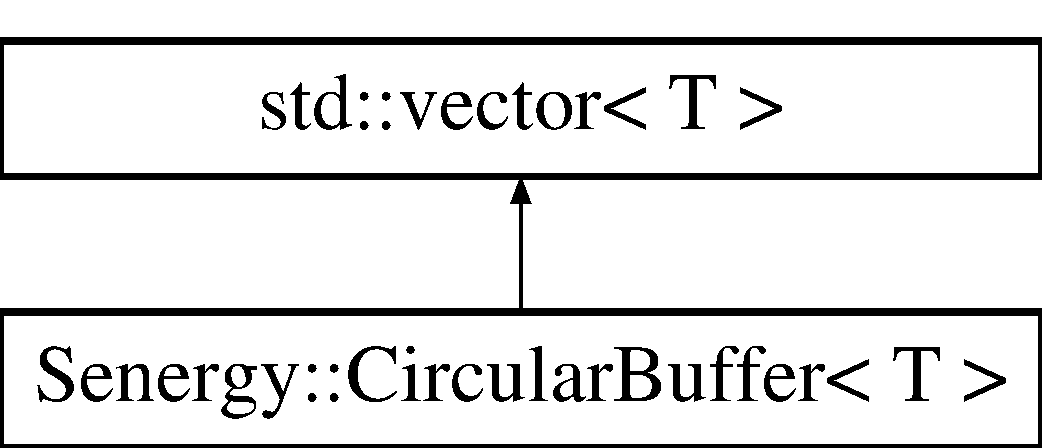
\includegraphics[height=2.000000cm]{class_senergy_1_1_circular_buffer}
\end{center}
\end{figure}
\subsection*{Public Member Functions}
\begin{DoxyCompactItemize}
\item 
\hyperlink{class_senergy_1_1_circular_buffer_abc3a5a67343d46ce83e2bbf678e83393}{Circular\-Buffer} (unsigned int size)
\begin{DoxyCompactList}\small\item\em Initializes a new instance of the \hyperlink{class_senergy_1_1_circular_buffer}{Circular\-Buffer} class with the specified size. \end{DoxyCompactList}\item 
void \hyperlink{class_senergy_1_1_circular_buffer_a26e52b6923a05022fcac2f825aa907cb}{push\-\_\-back} (T value)
\begin{DoxyCompactList}\small\item\em Overrides the vector's push\-\_\-back function, but makes sure no new entries are inserted. \end{DoxyCompactList}\end{DoxyCompactItemize}


\subsection{Detailed Description}
\subsubsection*{template$<$class T$>$class Senergy\-::\-Circular\-Buffer$<$ T $>$}

Simple circular buffer which uses a vector, simple circular buffer which should not be used in situations that require efficiency and power. 

T The type of data the circular buffer should hold.

\begin{DoxyNote}{Note}
The documentation does not explain how a circular buffer works. Please use Google for that.
\end{DoxyNote}
\begin{DoxyAuthor}{Author}
Swen Kooij (Photonios) 
\end{DoxyAuthor}


Definition at line 42 of file circular\-\_\-buffer.\-h.



\subsection{Constructor \& Destructor Documentation}
\hypertarget{class_senergy_1_1_circular_buffer_abc3a5a67343d46ce83e2bbf678e83393}{\index{Senergy\-::\-Circular\-Buffer@{Senergy\-::\-Circular\-Buffer}!Circular\-Buffer@{Circular\-Buffer}}
\index{Circular\-Buffer@{Circular\-Buffer}!Senergy::CircularBuffer@{Senergy\-::\-Circular\-Buffer}}
\subsubsection[{Circular\-Buffer}]{\setlength{\rightskip}{0pt plus 5cm}template$<$class T $>$ {\bf Senergy\-::\-Circular\-Buffer}$<$ T $>$\-::{\bf Circular\-Buffer} (
\begin{DoxyParamCaption}
\item[{unsigned int}]{size}
\end{DoxyParamCaption}
)\hspace{0.3cm}{\ttfamily [inline]}}}\label{class_senergy_1_1_circular_buffer_abc3a5a67343d46ce83e2bbf678e83393}


Initializes a new instance of the \hyperlink{class_senergy_1_1_circular_buffer}{Circular\-Buffer} class with the specified size. 



Definition at line 49 of file circular\-\_\-buffer.\-h.



\subsection{Member Function Documentation}
\hypertarget{class_senergy_1_1_circular_buffer_a26e52b6923a05022fcac2f825aa907cb}{\index{Senergy\-::\-Circular\-Buffer@{Senergy\-::\-Circular\-Buffer}!push\-\_\-back@{push\-\_\-back}}
\index{push\-\_\-back@{push\-\_\-back}!Senergy::CircularBuffer@{Senergy\-::\-Circular\-Buffer}}
\subsubsection[{push\-\_\-back}]{\setlength{\rightskip}{0pt plus 5cm}template$<$class T $>$ void {\bf Senergy\-::\-Circular\-Buffer}$<$ T $>$\-::push\-\_\-back (
\begin{DoxyParamCaption}
\item[{T}]{value}
\end{DoxyParamCaption}
)\hspace{0.3cm}{\ttfamily [inline]}}}\label{class_senergy_1_1_circular_buffer_a26e52b6923a05022fcac2f825aa907cb}


Overrides the vector's push\-\_\-back function, but makes sure no new entries are inserted. 


\begin{DoxyParams}{Parameters}
{\em value} & The value to insert into the circular buffer. \\
\hline
\end{DoxyParams}


Definition at line 62 of file circular\-\_\-buffer.\-h.



The documentation for this class was generated from the following file\-:\begin{DoxyCompactItemize}
\item 
src/senergy/\hyperlink{circular__buffer_8h}{circular\-\_\-buffer.\-h}\end{DoxyCompactItemize}

\hypertarget{class_senergy_1_1_convert}{\section{Senergy\-:\-:Convert Class Reference}
\label{class_senergy_1_1_convert}\index{Senergy\-::\-Convert@{Senergy\-::\-Convert}}
}


A simple conversion class, which simplifies conversion between various native data types. Based on the idea of the '\hyperlink{class_senergy_1_1_convert}{Convert}' class in the .N\-E\-T framework.  




{\ttfamily \#include $<$convert.\-h$>$}

\subsection*{Static Public Member Functions}
\begin{DoxyCompactItemize}
\item 
static std\-::string \hyperlink{class_senergy_1_1_convert_a80cf7b84b0ff65171da68ca40cbf817f}{To\-String} (int value)
\begin{DoxyCompactList}\small\item\em Converts the specified integer value to a string. \end{DoxyCompactList}\end{DoxyCompactItemize}


\subsection{Detailed Description}
A simple conversion class, which simplifies conversion between various native data types. Based on the idea of the '\hyperlink{class_senergy_1_1_convert}{Convert}' class in the .N\-E\-T framework. 

\begin{DoxyAuthor}{Author}
Swen Kooij (Photonios) 
\end{DoxyAuthor}


\subsection{Member Function Documentation}
\hypertarget{class_senergy_1_1_convert_a80cf7b84b0ff65171da68ca40cbf817f}{\index{Senergy\-::\-Convert@{Senergy\-::\-Convert}!To\-String@{To\-String}}
\index{To\-String@{To\-String}!Senergy::Convert@{Senergy\-::\-Convert}}
\subsubsection[{To\-String}]{\setlength{\rightskip}{0pt plus 5cm}std\-::string Senergy\-::\-Convert\-::\-To\-String (
\begin{DoxyParamCaption}
\item[{int}]{value}
\end{DoxyParamCaption}
)\hspace{0.3cm}{\ttfamily [static]}}}\label{class_senergy_1_1_convert_a80cf7b84b0ff65171da68ca40cbf817f}


Converts the specified integer value to a string. 


\begin{DoxyParams}{Parameters}
{\em value} & The integer value to convert to a string.\\
\hline
\end{DoxyParams}
\begin{DoxyReturn}{Returns}
The specified integer value as a string. 
\end{DoxyReturn}


The documentation for this class was generated from the following files\-:\begin{DoxyCompactItemize}
\item 
src/senergy/\hyperlink{convert_8h}{convert.\-h}\item 
src/\hyperlink{convert_8cpp}{convert.\-cpp}\end{DoxyCompactItemize}

\hypertarget{class_senergy_1_1_dns_1_1_id_factory}{\section{Senergy\-:\-:Dns\-:\-:Id\-Factory Class Reference}
\label{class_senergy_1_1_dns_1_1_id_factory}\index{Senergy\-::\-Dns\-::\-Id\-Factory@{Senergy\-::\-Dns\-::\-Id\-Factory}}
}


Static global factory that is used to generate random identifiers for D\-N\-S messages/packets. This is to ensure, each I\-D that is generated is unique.  




{\ttfamily \#include $<$id\-\_\-factory.\-h$>$}

\subsection*{Static Public Member Functions}
\begin{DoxyCompactItemize}
\item 
static unsigned short \hyperlink{class_senergy_1_1_dns_1_1_id_factory_aac705471a570313494ca2661a5888b3d}{Generate\-Id} ()
\begin{DoxyCompactList}\small\item\em Generates a new random identifier to be used as the unique identifier for a D\-N\-S message/packet. \end{DoxyCompactList}\end{DoxyCompactItemize}
\subsection*{Static Public Attributes}
\begin{DoxyCompactItemize}
\item 
static int \hyperlink{class_senergy_1_1_dns_1_1_id_factory_ae3169f3201faed02512868b1f128bbcb}{Maximum\-Buffer\-Size} = 20
\begin{DoxyCompactList}\small\item\em Defines the maximum number of generated I\-D's that we keep in our buffer, before we throw them out. \end{DoxyCompactList}\end{DoxyCompactItemize}


\subsection{Detailed Description}
Static global factory that is used to generate random identifiers for D\-N\-S messages/packets. This is to ensure, each I\-D that is generated is unique. 

\begin{DoxyNote}{Note}
This static class is thread-\/safe.
\end{DoxyNote}
\begin{DoxyAuthor}{Author}
Swen Kooij (Photonios) 
\end{DoxyAuthor}


Definition at line 44 of file id\-\_\-factory.\-h.



\subsection{Member Function Documentation}
\hypertarget{class_senergy_1_1_dns_1_1_id_factory_aac705471a570313494ca2661a5888b3d}{\index{Senergy\-::\-Dns\-::\-Id\-Factory@{Senergy\-::\-Dns\-::\-Id\-Factory}!Generate\-Id@{Generate\-Id}}
\index{Generate\-Id@{Generate\-Id}!Senergy::Dns::IdFactory@{Senergy\-::\-Dns\-::\-Id\-Factory}}
\subsubsection[{Generate\-Id}]{\setlength{\rightskip}{0pt plus 5cm}unsigned short Senergy\-::\-Dns\-::\-Id\-Factory\-::\-Generate\-Id (
\begin{DoxyParamCaption}
{}
\end{DoxyParamCaption}
)\hspace{0.3cm}{\ttfamily [static]}}}\label{class_senergy_1_1_dns_1_1_id_factory_aac705471a570313494ca2661a5888b3d}


Generates a new random identifier to be used as the unique identifier for a D\-N\-S message/packet. 

\begin{DoxyReturn}{Returns}
A unique, random identifier for a D\-N\-S message/packet. 
\end{DoxyReturn}


Definition at line 37 of file dns\-\_\-id\-\_\-factory.\-cpp.



\subsection{Member Data Documentation}
\hypertarget{class_senergy_1_1_dns_1_1_id_factory_ae3169f3201faed02512868b1f128bbcb}{\index{Senergy\-::\-Dns\-::\-Id\-Factory@{Senergy\-::\-Dns\-::\-Id\-Factory}!Maximum\-Buffer\-Size@{Maximum\-Buffer\-Size}}
\index{Maximum\-Buffer\-Size@{Maximum\-Buffer\-Size}!Senergy::Dns::IdFactory@{Senergy\-::\-Dns\-::\-Id\-Factory}}
\subsubsection[{Maximum\-Buffer\-Size}]{\setlength{\rightskip}{0pt plus 5cm}int Senergy\-::\-Dns\-::\-Id\-Factory\-::\-Maximum\-Buffer\-Size = 20\hspace{0.3cm}{\ttfamily [static]}}}\label{class_senergy_1_1_dns_1_1_id_factory_ae3169f3201faed02512868b1f128bbcb}


Defines the maximum number of generated I\-D's that we keep in our buffer, before we throw them out. 



Definition at line 51 of file id\-\_\-factory.\-h.



The documentation for this class was generated from the following files\-:\begin{DoxyCompactItemize}
\item 
src/senergy/dns/\hyperlink{id__factory_8h}{id\-\_\-factory.\-h}\item 
src/\hyperlink{dns__id__factory_8cpp}{dns\-\_\-id\-\_\-factory.\-cpp}\end{DoxyCompactItemize}

\hypertarget{class_senergy_1_1_dns_1_1_records_1_1_i_p_v4_address}{\section{Senergy\-:\-:Dns\-:\-:Records\-:\-:I\-P\-V4\-Address Class Reference}
\label{class_senergy_1_1_dns_1_1_records_1_1_i_p_v4_address}\index{Senergy\-::\-Dns\-::\-Records\-::\-I\-P\-V4\-Address@{Senergy\-::\-Dns\-::\-Records\-::\-I\-P\-V4\-Address}}
}


An address record, contains the answer to a lookup. Contains a I\-P\-V4 I\-P address, the response to a question, to lookup a hostname/domain name. This is part of a resource record, and the actual data is stored in the last field of a recource record (R\-D\-A\-T\-E). See the Resource\-Class and section 3.\-4.\-1 of R\-F\-C 1035 for more information.  




{\ttfamily \#include $<$record\-\_\-ipv4address.\-h$>$}

\subsection*{Public Member Functions}
\begin{DoxyCompactItemize}
\item 
\hyperlink{class_senergy_1_1_dns_1_1_records_1_1_i_p_v4_address_a71d523f7516849bf8e43981d5ec44ca8}{I\-P\-V4\-Address} (\hyperlink{namespace_senergy_1_1_dns_a1fa04259a07ce7a270e09288aa456ffd}{Resource\-Record\-Ptr} resource\-\_\-record)
\begin{DoxyCompactList}\small\item\em Initializes a new instance of the \hyperlink{class_senergy_1_1_dns_1_1_records_1_1_i_p_v4_address}{I\-P\-V4\-Address} class with the specified resource record. \end{DoxyCompactList}\item 
bool \hyperlink{class_senergy_1_1_dns_1_1_records_1_1_i_p_v4_address_a8de88ac0b61886638f63dd4930b07b36}{Deserialize} (\hyperlink{class_senergy_1_1_byte_buffer}{Byte\-Buffer} \&buffer)
\begin{DoxyCompactList}\small\item\em Deserializes the R\-D\-A\-T\-A part of this resource record, and does N\-O\-T deserialize the first part of the resource record. \end{DoxyCompactList}\item 
bool \hyperlink{class_senergy_1_1_dns_1_1_records_1_1_i_p_v4_address_ab080902a8a40e1933d327ff95298a996}{Serialize} (\hyperlink{class_senergy_1_1_byte_buffer}{Byte\-Buffer} \&buffer)
\begin{DoxyCompactList}\small\item\em Serializes the R\-D\-A\-T\-A part of this resource record, and does N\-O\-T serialize the first part of the resource record. \end{DoxyCompactList}\item 
void \hyperlink{class_senergy_1_1_dns_1_1_records_1_1_i_p_v4_address_a6d45ba035f7ff475f78a29593a6af0d5}{Dump} ()
\begin{DoxyCompactList}\small\item\em Dumps all fields to the standard output, with their values. In the following format\-: \end{DoxyCompactList}\end{DoxyCompactItemize}
\subsection*{Static Public Member Functions}
\begin{DoxyCompactItemize}
\item 
static I\-P\-V4\-Address\-Ptr \hyperlink{class_senergy_1_1_dns_1_1_records_1_1_i_p_v4_address_a6fefbdd798db0e2e33b66af9fde0c33f}{Create} (\hyperlink{namespace_senergy_1_1_dns_a1fa04259a07ce7a270e09288aa456ffd}{Resource\-Record\-Ptr} resource\-\_\-record)
\begin{DoxyCompactList}\small\item\em Initializes a new instance of the \hyperlink{class_senergy_1_1_dns_1_1_records_1_1_i_p_v4_address}{I\-P\-V4\-Address} class as a shared pointer. \end{DoxyCompactList}\end{DoxyCompactItemize}


\subsection{Detailed Description}
An address record, contains the answer to a lookup. Contains a I\-P\-V4 I\-P address, the response to a question, to lookup a hostname/domain name. This is part of a resource record, and the actual data is stored in the last field of a recource record (R\-D\-A\-T\-E). See the Resource\-Class and section 3.\-4.\-1 of R\-F\-C 1035 for more information. 

\begin{DoxyNote}{Note}
This is coupled with the \hyperlink{namespace_senergy_1_1_dns_a590bfd748c955364770f5ce358d9dfe0a7fc56270e7a70fa81a5935b72eacbe29}{Resource\-Record\-Type\-::\-A} type.
\end{DoxyNote}
\begin{DoxyAuthor}{Author}
Swen Kooij (Photonios) 
\end{DoxyAuthor}


Definition at line 50 of file record\-\_\-ipv4address.\-h.



\subsection{Constructor \& Destructor Documentation}
\hypertarget{class_senergy_1_1_dns_1_1_records_1_1_i_p_v4_address_a71d523f7516849bf8e43981d5ec44ca8}{\index{Senergy\-::\-Dns\-::\-Records\-::\-I\-P\-V4\-Address@{Senergy\-::\-Dns\-::\-Records\-::\-I\-P\-V4\-Address}!I\-P\-V4\-Address@{I\-P\-V4\-Address}}
\index{I\-P\-V4\-Address@{I\-P\-V4\-Address}!Senergy::Dns::Records::IPV4Address@{Senergy\-::\-Dns\-::\-Records\-::\-I\-P\-V4\-Address}}
\subsubsection[{I\-P\-V4\-Address}]{\setlength{\rightskip}{0pt plus 5cm}Senergy\-::\-Dns\-::\-Records\-::\-I\-P\-V4\-Address\-::\-I\-P\-V4\-Address (
\begin{DoxyParamCaption}
\item[{{\bf Resource\-Record\-Ptr}}]{resource\-\_\-record}
\end{DoxyParamCaption}
)}}\label{class_senergy_1_1_dns_1_1_records_1_1_i_p_v4_address_a71d523f7516849bf8e43981d5ec44ca8}


Initializes a new instance of the \hyperlink{class_senergy_1_1_dns_1_1_records_1_1_i_p_v4_address}{I\-P\-V4\-Address} class with the specified resource record. 


\begin{DoxyParams}{Parameters}
{\em resource\-\_\-record} & The resource record to use as a base for this instance. \\
\hline
\end{DoxyParams}


Definition at line 31 of file dns\-\_\-record\-\_\-ipv4address.\-cpp.



\subsection{Member Function Documentation}
\hypertarget{class_senergy_1_1_dns_1_1_records_1_1_i_p_v4_address_a6fefbdd798db0e2e33b66af9fde0c33f}{\index{Senergy\-::\-Dns\-::\-Records\-::\-I\-P\-V4\-Address@{Senergy\-::\-Dns\-::\-Records\-::\-I\-P\-V4\-Address}!Create@{Create}}
\index{Create@{Create}!Senergy::Dns::Records::IPV4Address@{Senergy\-::\-Dns\-::\-Records\-::\-I\-P\-V4\-Address}}
\subsubsection[{Create}]{\setlength{\rightskip}{0pt plus 5cm}I\-P\-V4\-Address\-Ptr Senergy\-::\-Dns\-::\-Records\-::\-I\-P\-V4\-Address\-::\-Create (
\begin{DoxyParamCaption}
\item[{{\bf Resource\-Record\-Ptr}}]{resource\-\_\-record}
\end{DoxyParamCaption}
)\hspace{0.3cm}{\ttfamily [static]}}}\label{class_senergy_1_1_dns_1_1_records_1_1_i_p_v4_address_a6fefbdd798db0e2e33b66af9fde0c33f}


Initializes a new instance of the \hyperlink{class_senergy_1_1_dns_1_1_records_1_1_i_p_v4_address}{I\-P\-V4\-Address} class as a shared pointer. 


\begin{DoxyParams}{Parameters}
{\em resource\-\_\-record} & The resource record to use as a base for this instance. \\
\hline
\end{DoxyParams}


Definition at line 36 of file dns\-\_\-record\-\_\-ipv4address.\-cpp.

\hypertarget{class_senergy_1_1_dns_1_1_records_1_1_i_p_v4_address_a8de88ac0b61886638f63dd4930b07b36}{\index{Senergy\-::\-Dns\-::\-Records\-::\-I\-P\-V4\-Address@{Senergy\-::\-Dns\-::\-Records\-::\-I\-P\-V4\-Address}!Deserialize@{Deserialize}}
\index{Deserialize@{Deserialize}!Senergy::Dns::Records::IPV4Address@{Senergy\-::\-Dns\-::\-Records\-::\-I\-P\-V4\-Address}}
\subsubsection[{Deserialize}]{\setlength{\rightskip}{0pt plus 5cm}bool Senergy\-::\-Dns\-::\-Records\-::\-I\-P\-V4\-Address\-::\-Deserialize (
\begin{DoxyParamCaption}
\item[{{\bf Byte\-Buffer} \&}]{buffer}
\end{DoxyParamCaption}
)}}\label{class_senergy_1_1_dns_1_1_records_1_1_i_p_v4_address_a8de88ac0b61886638f63dd4930b07b36}


Deserializes the R\-D\-A\-T\-A part of this resource record, and does N\-O\-T deserialize the first part of the resource record. 


\begin{DoxyParams}{Parameters}
{\em resource\-\_\-record} & The resource record to use as the base. \\
\hline
{\em buffer} & The buffer to read from.\\
\hline
\end{DoxyParams}
\begin{DoxyReturn}{Returns}
A boolean indicating whether this operation was a success. If the operation failed, false is returned. When the operation was a success, true is returned. 
\end{DoxyReturn}


Definition at line 41 of file dns\-\_\-record\-\_\-ipv4address.\-cpp.

\hypertarget{class_senergy_1_1_dns_1_1_records_1_1_i_p_v4_address_a6d45ba035f7ff475f78a29593a6af0d5}{\index{Senergy\-::\-Dns\-::\-Records\-::\-I\-P\-V4\-Address@{Senergy\-::\-Dns\-::\-Records\-::\-I\-P\-V4\-Address}!Dump@{Dump}}
\index{Dump@{Dump}!Senergy::Dns::Records::IPV4Address@{Senergy\-::\-Dns\-::\-Records\-::\-I\-P\-V4\-Address}}
\subsubsection[{Dump}]{\setlength{\rightskip}{0pt plus 5cm}void Senergy\-::\-Dns\-::\-Records\-::\-I\-P\-V4\-Address\-::\-Dump (
\begin{DoxyParamCaption}
{}
\end{DoxyParamCaption}
)}}\label{class_senergy_1_1_dns_1_1_records_1_1_i_p_v4_address_a6d45ba035f7ff475f78a29593a6af0d5}


Dumps all fields to the standard output, with their values. In the following format\-: 



Definition at line 68 of file dns\-\_\-record\-\_\-ipv4address.\-cpp.

\hypertarget{class_senergy_1_1_dns_1_1_records_1_1_i_p_v4_address_ab080902a8a40e1933d327ff95298a996}{\index{Senergy\-::\-Dns\-::\-Records\-::\-I\-P\-V4\-Address@{Senergy\-::\-Dns\-::\-Records\-::\-I\-P\-V4\-Address}!Serialize@{Serialize}}
\index{Serialize@{Serialize}!Senergy::Dns::Records::IPV4Address@{Senergy\-::\-Dns\-::\-Records\-::\-I\-P\-V4\-Address}}
\subsubsection[{Serialize}]{\setlength{\rightskip}{0pt plus 5cm}bool Senergy\-::\-Dns\-::\-Records\-::\-I\-P\-V4\-Address\-::\-Serialize (
\begin{DoxyParamCaption}
\item[{{\bf Byte\-Buffer} \&}]{buffer}
\end{DoxyParamCaption}
)}}\label{class_senergy_1_1_dns_1_1_records_1_1_i_p_v4_address_ab080902a8a40e1933d327ff95298a996}


Serializes the R\-D\-A\-T\-A part of this resource record, and does N\-O\-T serialize the first part of the resource record. 


\begin{DoxyParams}{Parameters}
{\em resource\-\_\-record} & The resource record to use as the base. \\
\hline
{\em buffer} & The buffer to write to.\\
\hline
\end{DoxyParams}
\begin{DoxyReturn}{Returns}
A boolean indicating whether this operation was a success. If the operation failed, false is returned. When the operation was a success, true is returned. 
\end{DoxyReturn}


Definition at line 61 of file dns\-\_\-record\-\_\-ipv4address.\-cpp.



The documentation for this class was generated from the following files\-:\begin{DoxyCompactItemize}
\item 
src/senergy/dns/\hyperlink{record__ipv4address_8h}{record\-\_\-ipv4address.\-h}\item 
src/\hyperlink{dns__record__ipv4address_8cpp}{dns\-\_\-record\-\_\-ipv4address.\-cpp}\end{DoxyCompactItemize}

\hypertarget{class_senergy_1_1_dns_1_1_message}{\section{Senergy\-:\-:Dns\-:\-:Message Class Reference}
\label{class_senergy_1_1_dns_1_1_message}\index{Senergy\-::\-Dns\-::\-Message@{Senergy\-::\-Dns\-::\-Message}}
}


Represents a D\-N\-S packet as described in section 4 of R\-F\-C-\/1035. A D\-N\-S packet is the standard message format that is transmitted and received by D\-N\-S clients and hosts.  




{\ttfamily \#include $<$message.\-h$>$}

\subsection*{Public Member Functions}
\begin{DoxyCompactItemize}
\item 
\hyperlink{class_senergy_1_1_dns_1_1_message_a3e7192f2293903a43e7d08960b08a8b1}{Message} ()
\begin{DoxyCompactList}\small\item\em Initializes a new instance of the \hyperlink{class_senergy_1_1_dns_1_1_message}{Message} class, with default values, without questions, answers, authorities and additionals. \end{DoxyCompactList}\item 
bool \hyperlink{class_senergy_1_1_dns_1_1_message_a3857764a799ab123405420345f9b03ee}{Deserialize} (\hyperlink{class_senergy_1_1_byte_buffer}{Byte\-Buffer} \&buffer)
\begin{DoxyCompactList}\small\item\em Deserializes a D\-N\-S packet header from the specified buffer into this instance. \end{DoxyCompactList}\item 
bool \hyperlink{class_senergy_1_1_dns_1_1_message_a2e7978e799fadaa4f03fc881e5c8e0f6}{Serialize} (\hyperlink{class_senergy_1_1_byte_buffer}{Byte\-Buffer} \&buffer)
\begin{DoxyCompactList}\small\item\em Serializes this D\-N\-S message (packet) into the specified \hyperlink{class_senergy_1_1_byte_buffer}{Byte\-Buffer}. \end{DoxyCompactList}\item 
void \hyperlink{class_senergy_1_1_dns_1_1_message_a60d242fef8b20993f9cd9b4591453e1b}{Reset} ()
\begin{DoxyCompactList}\small\item\em Resets this message so that all vectors/collections will be cleared, and default values restored. \end{DoxyCompactList}\item 
int \hyperlink{class_senergy_1_1_dns_1_1_message_a5d5219532098cf60e2395764e7f61aca}{Get\-Question\-Count} ()
\begin{DoxyCompactList}\small\item\em Gets the amount of questions this D\-N\-S message currently holds. \end{DoxyCompactList}\end{DoxyCompactItemize}
\subsection*{Public Attributes}
\begin{DoxyCompactItemize}
\item 
\hyperlink{namespace_senergy_1_1_dns_a76982150ca0b86c08d888f3e3e805747}{Message\-Question\-Ptr\-Vector} \hyperlink{class_senergy_1_1_dns_1_1_message_a1e72009ea8004f0e8cc1ce0ea07f4ad1}{Questions}
\begin{DoxyCompactList}\small\item\em Holds all the 'question messages' that are part of this D\-N\-S message. \end{DoxyCompactList}\end{DoxyCompactItemize}


\subsection{Detailed Description}
Represents a D\-N\-S packet as described in section 4 of R\-F\-C-\/1035. A D\-N\-S packet is the standard message format that is transmitted and received by D\-N\-S clients and hosts. 

\begin{DoxyAuthor}{Author}
Swen Kooij (Photonios) 
\end{DoxyAuthor}


Definition at line 41 of file message.\-h.



\subsection{Constructor \& Destructor Documentation}
\hypertarget{class_senergy_1_1_dns_1_1_message_a3e7192f2293903a43e7d08960b08a8b1}{\index{Senergy\-::\-Dns\-::\-Message@{Senergy\-::\-Dns\-::\-Message}!Message@{Message}}
\index{Message@{Message}!Senergy::Dns::Message@{Senergy\-::\-Dns\-::\-Message}}
\subsubsection[{Message}]{\setlength{\rightskip}{0pt plus 5cm}Senergy\-::\-Dns\-::\-Message\-::\-Message (
\begin{DoxyParamCaption}
{}
\end{DoxyParamCaption}
)}}\label{class_senergy_1_1_dns_1_1_message_a3e7192f2293903a43e7d08960b08a8b1}


Initializes a new instance of the \hyperlink{class_senergy_1_1_dns_1_1_message}{Message} class, with default values, without questions, answers, authorities and additionals. 



Definition at line 29 of file message.\-cpp.



\subsection{Member Function Documentation}
\hypertarget{class_senergy_1_1_dns_1_1_message_a3857764a799ab123405420345f9b03ee}{\index{Senergy\-::\-Dns\-::\-Message@{Senergy\-::\-Dns\-::\-Message}!Deserialize@{Deserialize}}
\index{Deserialize@{Deserialize}!Senergy::Dns::Message@{Senergy\-::\-Dns\-::\-Message}}
\subsubsection[{Deserialize}]{\setlength{\rightskip}{0pt plus 5cm}bool Senergy\-::\-Dns\-::\-Message\-::\-Deserialize (
\begin{DoxyParamCaption}
\item[{{\bf Byte\-Buffer} \&}]{buffer}
\end{DoxyParamCaption}
)}}\label{class_senergy_1_1_dns_1_1_message_a3857764a799ab123405420345f9b03ee}


Deserializes a D\-N\-S packet header from the specified buffer into this instance. 

\begin{DoxyNote}{Note}
The D\-N\-S packet header is 12 bytes, the specified buffer should have at least 12 bytes left to read. Deserialization will fail when there are less then 12 bytes left to read.

This will overwrite all contents currently in this message.

If the operation suceseeded, the buffer's position will have at least advanced 12 bytes.
\end{DoxyNote}

\begin{DoxyParams}{Parameters}
{\em buffer} & The buffer to read from, should contain a D\-N\-S packet message.\\
\hline
\end{DoxyParams}
\begin{DoxyReturn}{Returns}
A boolean indicating whether deserialization was succesfull. True is returned when it was a success and false is returned when it failed. 
\end{DoxyReturn}


Definition at line 33 of file message.\-cpp.

\hypertarget{class_senergy_1_1_dns_1_1_message_a5d5219532098cf60e2395764e7f61aca}{\index{Senergy\-::\-Dns\-::\-Message@{Senergy\-::\-Dns\-::\-Message}!Get\-Question\-Count@{Get\-Question\-Count}}
\index{Get\-Question\-Count@{Get\-Question\-Count}!Senergy::Dns::Message@{Senergy\-::\-Dns\-::\-Message}}
\subsubsection[{Get\-Question\-Count}]{\setlength{\rightskip}{0pt plus 5cm}int Senergy\-::\-Dns\-::\-Message\-::\-Get\-Question\-Count (
\begin{DoxyParamCaption}
{}
\end{DoxyParamCaption}
)}}\label{class_senergy_1_1_dns_1_1_message_a5d5219532098cf60e2395764e7f61aca}


Gets the amount of questions this D\-N\-S message currently holds. 

\begin{DoxyReturn}{Returns}
The amount of questions this D\-N\-S message currently holds. 
\end{DoxyReturn}


Definition at line 87 of file message.\-cpp.

\hypertarget{class_senergy_1_1_dns_1_1_message_a60d242fef8b20993f9cd9b4591453e1b}{\index{Senergy\-::\-Dns\-::\-Message@{Senergy\-::\-Dns\-::\-Message}!Reset@{Reset}}
\index{Reset@{Reset}!Senergy::Dns::Message@{Senergy\-::\-Dns\-::\-Message}}
\subsubsection[{Reset}]{\setlength{\rightskip}{0pt plus 5cm}void Senergy\-::\-Dns\-::\-Message\-::\-Reset (
\begin{DoxyParamCaption}
{}
\end{DoxyParamCaption}
)}}\label{class_senergy_1_1_dns_1_1_message_a60d242fef8b20993f9cd9b4591453e1b}


Resets this message so that all vectors/collections will be cleared, and default values restored. 



Definition at line 82 of file message.\-cpp.

\hypertarget{class_senergy_1_1_dns_1_1_message_a2e7978e799fadaa4f03fc881e5c8e0f6}{\index{Senergy\-::\-Dns\-::\-Message@{Senergy\-::\-Dns\-::\-Message}!Serialize@{Serialize}}
\index{Serialize@{Serialize}!Senergy::Dns::Message@{Senergy\-::\-Dns\-::\-Message}}
\subsubsection[{Serialize}]{\setlength{\rightskip}{0pt plus 5cm}bool Senergy\-::\-Dns\-::\-Message\-::\-Serialize (
\begin{DoxyParamCaption}
\item[{{\bf Byte\-Buffer} \&}]{buffer}
\end{DoxyParamCaption}
)}}\label{class_senergy_1_1_dns_1_1_message_a2e7978e799fadaa4f03fc881e5c8e0f6}


Serializes this D\-N\-S message (packet) into the specified \hyperlink{class_senergy_1_1_byte_buffer}{Byte\-Buffer}. 


\begin{DoxyParams}{Parameters}
{\em buffer} & The buffer to write the serialized D\-N\-S message to.\\
\hline
\end{DoxyParams}
\begin{DoxyReturn}{Returns}
A boolean indicating whether serialization was succesfull. True is returned when it was a success and false is returned when it failed. 
\end{DoxyReturn}


Definition at line 58 of file message.\-cpp.



\subsection{Member Data Documentation}
\hypertarget{class_senergy_1_1_dns_1_1_message_a1e72009ea8004f0e8cc1ce0ea07f4ad1}{\index{Senergy\-::\-Dns\-::\-Message@{Senergy\-::\-Dns\-::\-Message}!Questions@{Questions}}
\index{Questions@{Questions}!Senergy::Dns::Message@{Senergy\-::\-Dns\-::\-Message}}
\subsubsection[{Questions}]{\setlength{\rightskip}{0pt plus 5cm}{\bf Message\-Question\-Ptr\-Vector} Senergy\-::\-Dns\-::\-Message\-::\-Questions}}\label{class_senergy_1_1_dns_1_1_message_a1e72009ea8004f0e8cc1ce0ea07f4ad1}


Holds all the 'question messages' that are part of this D\-N\-S message. 



Definition at line 97 of file message.\-h.



The documentation for this class was generated from the following files\-:\begin{DoxyCompactItemize}
\item 
src/senergy/dns/\hyperlink{message_8h}{message.\-h}\item 
src/\hyperlink{message_8cpp}{message.\-cpp}\end{DoxyCompactItemize}

\hypertarget{class_senergy_1_1_dns_1_1_message_header}{\section{Senergy\-:\-:Dns\-:\-:Message\-Header Class Reference}
\label{class_senergy_1_1_dns_1_1_message_header}\index{Senergy\-::\-Dns\-::\-Message\-Header@{Senergy\-::\-Dns\-::\-Message\-Header}}
}


Defines the header of a D\-N\-S packet, as described in section 4.\-1 of R\-F\-C-\/1035. All D\-N\-S messages start with this header.  




{\ttfamily \#include $<$message\-\_\-header.\-h$>$}

\subsection*{Public Member Functions}
\begin{DoxyCompactItemize}
\item 
\hyperlink{class_senergy_1_1_dns_1_1_message_header_aa103a12edc759b885f57728c091a84eb}{Message\-Header} ()
\begin{DoxyCompactList}\small\item\em Initializes a new instance of the \hyperlink{class_senergy_1_1_dns_1_1_message_header}{Message\-Header} class, with the default values. \end{DoxyCompactList}\item 
bool \hyperlink{class_senergy_1_1_dns_1_1_message_header_a3636da2fa7e96513080d1985ef515958}{Is\-Valid} ()
\begin{DoxyCompactList}\small\item\em Gets whether this instance is a valid D\-N\-S packet header. \end{DoxyCompactList}\item 
int \hyperlink{class_senergy_1_1_dns_1_1_message_header_a69f4475bc3153926dbb011f37cbbfea9}{Get\-Size} ()
\begin{DoxyCompactList}\small\item\em Gets the size of a D\-N\-S packet header. This is almost constant as long as the \hyperlink{struct_senergy_1_1_dns_1_1_message_header_fields}{Message\-Header\-Fields} structure doesn't change. \end{DoxyCompactList}\item 
bool \hyperlink{class_senergy_1_1_dns_1_1_message_header_ab443595ff8e11a828022f0cc5f3f6fbe}{Serialize} (\hyperlink{class_senergy_1_1_byte_buffer}{Byte\-Buffer} \&buffer)
\begin{DoxyCompactList}\small\item\em Serializes this instance into the specified buffer, ready for transmission. \end{DoxyCompactList}\end{DoxyCompactItemize}
\subsection*{Static Public Member Functions}
\begin{DoxyCompactItemize}
\item 
static \hyperlink{class_senergy_1_1_dns_1_1_message_header}{Message\-Header} \hyperlink{class_senergy_1_1_dns_1_1_message_header_aec3c0b3f2af0504bfa8fca6562c5b039}{Deserialize} (\hyperlink{class_senergy_1_1_byte_buffer}{Byte\-Buffer} \&buffer)
\begin{DoxyCompactList}\small\item\em Deserializes a D\-N\-S packet header from the specified buffer and returns the deserialized result as an instance of the \hyperlink{class_senergy_1_1_dns_1_1_message_header}{Message\-Header} class. \end{DoxyCompactList}\end{DoxyCompactItemize}
\subsection*{Public Attributes}
\begin{DoxyCompactItemize}
\item 
\hyperlink{struct_senergy_1_1_dns_1_1_message_header_fields}{Message\-Header\-Fields} \hyperlink{class_senergy_1_1_dns_1_1_message_header_a014c173ce2b2c5bb06ae9e5d0e201159}{Fields}
\begin{DoxyCompactList}\small\item\em The fields that are part of a D\-N\-S packet header. See \hyperlink{struct_senergy_1_1_dns_1_1_message_header_fields}{Message\-Header\-Fields} for a complete list. This contains the actual data that is transmitted and received. \end{DoxyCompactList}\end{DoxyCompactItemize}


\subsection{Detailed Description}
Defines the header of a D\-N\-S packet, as described in section 4.\-1 of R\-F\-C-\/1035. All D\-N\-S messages start with this header. 

\begin{DoxyNote}{Note}
The actual data will be within a \hyperlink{struct_senergy_1_1_dns_1_1_message_header_fields}{Message\-Header\-Fields} data structure.
\end{DoxyNote}
\begin{DoxySeeAlso}{See Also}
\href{http://msdn.microsoft.com/en-us/library/windows/desktop/ms682059(v=vs.85).aspx}{\tt http\-://msdn.\-microsoft.\-com/en-\/us/library/windows/desktop/ms682059(v=vs.\-85).\-aspx} 

\href{http://www.ietf.org/rfc/rfc1035.txt}{\tt http\-://www.\-ietf.\-org/rfc/rfc1035.\-txt}
\end{DoxySeeAlso}
\begin{DoxyAuthor}{Author}
Swen Kooij (Photonios) 
\end{DoxyAuthor}


Definition at line 207 of file message\-\_\-header.\-h.



\subsection{Constructor \& Destructor Documentation}
\hypertarget{class_senergy_1_1_dns_1_1_message_header_aa103a12edc759b885f57728c091a84eb}{\index{Senergy\-::\-Dns\-::\-Message\-Header@{Senergy\-::\-Dns\-::\-Message\-Header}!Message\-Header@{Message\-Header}}
\index{Message\-Header@{Message\-Header}!Senergy::Dns::MessageHeader@{Senergy\-::\-Dns\-::\-Message\-Header}}
\subsubsection[{Message\-Header}]{\setlength{\rightskip}{0pt plus 5cm}Senergy\-::\-Dns\-::\-Message\-Header\-::\-Message\-Header (
\begin{DoxyParamCaption}
{}
\end{DoxyParamCaption}
)}}\label{class_senergy_1_1_dns_1_1_message_header_aa103a12edc759b885f57728c091a84eb}


Initializes a new instance of the \hyperlink{class_senergy_1_1_dns_1_1_message_header}{Message\-Header} class, with the default values. 



Definition at line 29 of file message\-\_\-header.\-cpp.



\subsection{Member Function Documentation}
\hypertarget{class_senergy_1_1_dns_1_1_message_header_aec3c0b3f2af0504bfa8fca6562c5b039}{\index{Senergy\-::\-Dns\-::\-Message\-Header@{Senergy\-::\-Dns\-::\-Message\-Header}!Deserialize@{Deserialize}}
\index{Deserialize@{Deserialize}!Senergy::Dns::MessageHeader@{Senergy\-::\-Dns\-::\-Message\-Header}}
\subsubsection[{Deserialize}]{\setlength{\rightskip}{0pt plus 5cm}{\bf Message\-Header} Senergy\-::\-Dns\-::\-Message\-Header\-::\-Deserialize (
\begin{DoxyParamCaption}
\item[{{\bf Byte\-Buffer} \&}]{buffer}
\end{DoxyParamCaption}
)\hspace{0.3cm}{\ttfamily [static]}}}\label{class_senergy_1_1_dns_1_1_message_header_aec3c0b3f2af0504bfa8fca6562c5b039}


Deserializes a D\-N\-S packet header from the specified buffer and returns the deserialized result as an instance of the \hyperlink{class_senergy_1_1_dns_1_1_message_header}{Message\-Header} class. 

\begin{DoxyNote}{Note}
The D\-N\-S message header is 12 bytes, the specified buffer must at least have 12 bytes left to read.

Using this will advance the position of the specified \hyperlink{class_senergy_1_1_byte_buffer}{Byte\-Buffer} with 12 bytes.
\end{DoxyNote}

\begin{DoxyParams}{Parameters}
{\em buffer} & A reference to an instance of the \hyperlink{class_senergy_1_1_byte_buffer}{Byte\-Buffer} class, the buffer to read from.\\
\hline
\end{DoxyParams}
\begin{DoxyReturn}{Returns}
An instance of the \hyperlink{class_senergy_1_1_dns_1_1_message_header}{Message\-Header} class, containing the deserialized D\-N\-S packet header. If deserialization failed, an invalid \hyperlink{class_senergy_1_1_dns_1_1_message_header}{Message\-Header} instance is returned. 
\end{DoxyReturn}


Definition at line 44 of file message\-\_\-header.\-cpp.

\hypertarget{class_senergy_1_1_dns_1_1_message_header_a69f4475bc3153926dbb011f37cbbfea9}{\index{Senergy\-::\-Dns\-::\-Message\-Header@{Senergy\-::\-Dns\-::\-Message\-Header}!Get\-Size@{Get\-Size}}
\index{Get\-Size@{Get\-Size}!Senergy::Dns::MessageHeader@{Senergy\-::\-Dns\-::\-Message\-Header}}
\subsubsection[{Get\-Size}]{\setlength{\rightskip}{0pt plus 5cm}int Senergy\-::\-Dns\-::\-Message\-Header\-::\-Get\-Size (
\begin{DoxyParamCaption}
{}
\end{DoxyParamCaption}
)}}\label{class_senergy_1_1_dns_1_1_message_header_a69f4475bc3153926dbb011f37cbbfea9}


Gets the size of a D\-N\-S packet header. This is almost constant as long as the \hyperlink{struct_senergy_1_1_dns_1_1_message_header_fields}{Message\-Header\-Fields} structure doesn't change. 

\begin{DoxyReturn}{Returns}
The size of a \hyperlink{struct_senergy_1_1_dns_1_1_message_header_fields}{Message\-Header\-Fields} structure, the size of a D\-N\-S packet header. 
\end{DoxyReturn}


Definition at line 39 of file message\-\_\-header.\-cpp.

\hypertarget{class_senergy_1_1_dns_1_1_message_header_a3636da2fa7e96513080d1985ef515958}{\index{Senergy\-::\-Dns\-::\-Message\-Header@{Senergy\-::\-Dns\-::\-Message\-Header}!Is\-Valid@{Is\-Valid}}
\index{Is\-Valid@{Is\-Valid}!Senergy::Dns::MessageHeader@{Senergy\-::\-Dns\-::\-Message\-Header}}
\subsubsection[{Is\-Valid}]{\setlength{\rightskip}{0pt plus 5cm}bool Senergy\-::\-Dns\-::\-Message\-Header\-::\-Is\-Valid (
\begin{DoxyParamCaption}
{}
\end{DoxyParamCaption}
)}}\label{class_senergy_1_1_dns_1_1_message_header_a3636da2fa7e96513080d1985ef515958}


Gets whether this instance is a valid D\-N\-S packet header. 

\begin{DoxyReturn}{Returns}
Whether this instance is a valid D\-N\-S packet header. True is returned when this instance is valid, and suited for transmission, and false is returned when this instance is invalid, and should not be used for transmission. 
\end{DoxyReturn}


Definition at line 34 of file message\-\_\-header.\-cpp.

\hypertarget{class_senergy_1_1_dns_1_1_message_header_ab443595ff8e11a828022f0cc5f3f6fbe}{\index{Senergy\-::\-Dns\-::\-Message\-Header@{Senergy\-::\-Dns\-::\-Message\-Header}!Serialize@{Serialize}}
\index{Serialize@{Serialize}!Senergy::Dns::MessageHeader@{Senergy\-::\-Dns\-::\-Message\-Header}}
\subsubsection[{Serialize}]{\setlength{\rightskip}{0pt plus 5cm}bool Senergy\-::\-Dns\-::\-Message\-Header\-::\-Serialize (
\begin{DoxyParamCaption}
\item[{{\bf Byte\-Buffer} \&}]{buffer}
\end{DoxyParamCaption}
)}}\label{class_senergy_1_1_dns_1_1_message_header_ab443595ff8e11a828022f0cc5f3f6fbe}


Serializes this instance into the specified buffer, ready for transmission. 

\begin{DoxyNote}{Note}
Serialization will fail when this instance is not valid.

Using this will advance the position of the specified \hyperlink{class_senergy_1_1_byte_buffer}{Byte\-Buffer} with 12 bytes.
\end{DoxyNote}

\begin{DoxyParams}{Parameters}
{\em buffer} & A reference to the \hyperlink{class_senergy_1_1_byte_buffer}{Byte\-Buffer} to write the serialized D\-N\-S packet header into.\\
\hline
\end{DoxyParams}
\begin{DoxyReturn}{Returns}
A boolean indicating whether serialization was sucessful. True is returned when seralization suceseeded and false is returned when it failed. 
\end{DoxyReturn}


Definition at line 61 of file message\-\_\-header.\-cpp.



\subsection{Member Data Documentation}
\hypertarget{class_senergy_1_1_dns_1_1_message_header_a014c173ce2b2c5bb06ae9e5d0e201159}{\index{Senergy\-::\-Dns\-::\-Message\-Header@{Senergy\-::\-Dns\-::\-Message\-Header}!Fields@{Fields}}
\index{Fields@{Fields}!Senergy::Dns::MessageHeader@{Senergy\-::\-Dns\-::\-Message\-Header}}
\subsubsection[{Fields}]{\setlength{\rightskip}{0pt plus 5cm}{\bf Message\-Header\-Fields} Senergy\-::\-Dns\-::\-Message\-Header\-::\-Fields}}\label{class_senergy_1_1_dns_1_1_message_header_a014c173ce2b2c5bb06ae9e5d0e201159}


The fields that are part of a D\-N\-S packet header. See \hyperlink{struct_senergy_1_1_dns_1_1_message_header_fields}{Message\-Header\-Fields} for a complete list. This contains the actual data that is transmitted and received. 



Definition at line 279 of file message\-\_\-header.\-h.



The documentation for this class was generated from the following files\-:\begin{DoxyCompactItemize}
\item 
src/senergy/dns/\hyperlink{message__header_8h}{message\-\_\-header.\-h}\item 
src/\hyperlink{message__header_8cpp}{message\-\_\-header.\-cpp}\end{DoxyCompactItemize}

\hypertarget{struct_senergy_1_1_dns_1_1_message_header_fields}{\section{Senergy\-:\-:Dns\-:\-:Message\-Header\-Fields Struct Reference}
\label{struct_senergy_1_1_dns_1_1_message_header_fields}\index{Senergy\-::\-Dns\-::\-Message\-Header\-Fields@{Senergy\-::\-Dns\-::\-Message\-Header\-Fields}}
}


Defines the fields within a D\-N\-S packet header, as described in section 4.\-1 of R\-F\-C-\/1035. This data structure is used as the \char`\"{}\-Fields\char`\"{} member/property of the \hyperlink{class_senergy_1_1_dns_1_1_message_header}{Message\-Header} class, and serves as the container of the actual data.  




{\ttfamily \#include $<$message\-\_\-header.\-h$>$}

\subsection*{Public Attributes}
\begin{DoxyCompactItemize}
\item 
unsigned short \hyperlink{struct_senergy_1_1_dns_1_1_message_header_fields_ab423a1e91fecd6ad2ec36a4bdafd5c2b}{Id}
\begin{DoxyCompactList}\small\item\em A 16 bit identifier assigned by the program that generates any kind of query. This identifier is copied the corresponding reply and can be used by the requester to match up replies to outstanding queries. \end{DoxyCompactList}\item 
unsigned char \hyperlink{struct_senergy_1_1_dns_1_1_message_header_fields_ab5d7c8933016bb7288462b4a0ac131a5}{Recursion\-Desired}\-:1
\begin{DoxyCompactList}\small\item\em Recursion Desired -\/ this bit may be set in a query and is copied into the response. If R\-D is set, it directs the name server to pursue the query recursively. Recursive query support is optional. \end{DoxyCompactList}\item 
unsigned char \hyperlink{struct_senergy_1_1_dns_1_1_message_header_fields_a15d1ee99bf788c080001c3216c88274c}{Truncation}\-:1
\begin{DoxyCompactList}\small\item\em Trun\-Cation -\/ specifies that this message was truncated due to length greater than that permitted on the transmission channel. \end{DoxyCompactList}\item 
unsigned char \hyperlink{struct_senergy_1_1_dns_1_1_message_header_fields_a706fe34b459a6aaacc28f0249213b013}{Authoritative}\-:1
\begin{DoxyCompactList}\small\item\em Authoritative Answer -\/ this bit is valid in responses, and specifies that the responding name server is an authority for the domain name in question section. \end{DoxyCompactList}\item 
unsigned char \hyperlink{struct_senergy_1_1_dns_1_1_message_header_fields_ac2d7ba4468405e5693f07d4321058be0}{Opcode}\-:4
\begin{DoxyCompactList}\small\item\em A four bit field that specifies kind of query in this message. This value is set by the originator of a query and copied into the response. The values are\-: \end{DoxyCompactList}\item 
unsigned char \hyperlink{struct_senergy_1_1_dns_1_1_message_header_fields_a0d0ac4fa85684c3d66a84e3392f3ef99}{Is\-Response}\-:1
\begin{DoxyCompactList}\small\item\em A one bit field that specifies whether this message is a query (0), or a response (1). \end{DoxyCompactList}\item 
unsigned char \hyperlink{struct_senergy_1_1_dns_1_1_message_header_fields_a2f42c94d4e50dd7a63b11c8b374597c4}{Response\-Code}\-:4
\begin{DoxyCompactList}\small\item\em Response code -\/ this 4 bit field is set as part of responses. The values have the following interpretation\-: \end{DoxyCompactList}\item 
unsigned char \hyperlink{struct_senergy_1_1_dns_1_1_message_header_fields_a2c846064b4582f46a94bd90b32ef1cd9}{Checking\-Disabled}\-:1
\item 
unsigned char \hyperlink{struct_senergy_1_1_dns_1_1_message_header_fields_a3788cbe9e2663b3be0cad8cbca8dc985}{Authenticated\-Data}\-:1
\begin{DoxyCompactList}\small\item\em A value that specifies whether the D\-N\-S data following the D\-N\-S packet header is authenticated by the D\-N\-S server. \end{DoxyCompactList}\item 
unsigned char \hyperlink{struct_senergy_1_1_dns_1_1_message_header_fields_afb988d15085d4f740df367d1792440c7}{Reserved}\-:1
\begin{DoxyCompactList}\small\item\em Reserved for future use. Must be zero in all queries and responses. \end{DoxyCompactList}\item 
unsigned char \hyperlink{struct_senergy_1_1_dns_1_1_message_header_fields_afbb68b60a28f855e64eb13615fc2633e}{Recursion\-Available}\-:1
\begin{DoxyCompactList}\small\item\em Recursion Available -\/ this be is set or cleared in a response, and denotes whether recursive query support is available in the name server. \end{DoxyCompactList}\item 
unsigned short \hyperlink{struct_senergy_1_1_dns_1_1_message_header_fields_a8af9bbfa134c9e0d4fc846103f7b72ad}{Question\-Count}
\begin{DoxyCompactList}\small\item\em An unsigned 16 bit integer specifying the number of entries in the question section. \end{DoxyCompactList}\item 
unsigned short \hyperlink{struct_senergy_1_1_dns_1_1_message_header_fields_a38e5101ec862c400628d66192c5b9878}{Answer\-Count}
\begin{DoxyCompactList}\small\item\em The number of resource records (R\-Rs) contained in the answer section of the D\-N\-S message. \end{DoxyCompactList}\item 
unsigned short \hyperlink{struct_senergy_1_1_dns_1_1_message_header_fields_a963b92841b3f7fc5fc9268c963d32d8d}{Name\-Server\-Count}
\begin{DoxyCompactList}\small\item\em The number of D\-N\-S name server R\-Rs contained in the authority section of the D\-N\-S message. This value is the number of D\-N\-S name servers the message has traversed in its search for resolution. \end{DoxyCompactList}\item 
unsigned short \hyperlink{struct_senergy_1_1_dns_1_1_message_header_fields_aae6ba21a1c8baa30f0aafe90d165420f}{Additional\-Count}
\begin{DoxyCompactList}\small\item\em Reserved. Do not use. \end{DoxyCompactList}\end{DoxyCompactItemize}


\subsection{Detailed Description}
Defines the fields within a D\-N\-S packet header, as described in section 4.\-1 of R\-F\-C-\/1035. This data structure is used as the \char`\"{}\-Fields\char`\"{} member/property of the \hyperlink{class_senergy_1_1_dns_1_1_message_header}{Message\-Header} class, and serves as the container of the actual data. 

\begin{DoxyNote}{Note}
This size of this structure is 12 bytes.
\end{DoxyNote}
\begin{DoxySeeAlso}{See Also}
\href{http://msdn.microsoft.com/en-us/library/windows/desktop/ms682059(v=vs.85).aspx}{\tt http\-://msdn.\-microsoft.\-com/en-\/us/library/windows/desktop/ms682059(v=vs.\-85).\-aspx} 

\href{http://www.ietf.org/rfc/rfc1035.txt}{\tt http\-://www.\-ietf.\-org/rfc/rfc1035.\-txt}
\end{DoxySeeAlso}
\begin{DoxyAuthor}{Author}
Swen Kooij (Photonios) 
\end{DoxyAuthor}


Definition at line 50 of file message\-\_\-header.\-h.



\subsection{Member Data Documentation}
\hypertarget{struct_senergy_1_1_dns_1_1_message_header_fields_aae6ba21a1c8baa30f0aafe90d165420f}{\index{Senergy\-::\-Dns\-::\-Message\-Header\-Fields@{Senergy\-::\-Dns\-::\-Message\-Header\-Fields}!Additional\-Count@{Additional\-Count}}
\index{Additional\-Count@{Additional\-Count}!Senergy::Dns::MessageHeaderFields@{Senergy\-::\-Dns\-::\-Message\-Header\-Fields}}
\subsubsection[{Additional\-Count}]{\setlength{\rightskip}{0pt plus 5cm}unsigned short Senergy\-::\-Dns\-::\-Message\-Header\-Fields\-::\-Additional\-Count}}\label{struct_senergy_1_1_dns_1_1_message_header_fields_aae6ba21a1c8baa30f0aafe90d165420f}


Reserved. Do not use. 



Definition at line 201 of file message\-\_\-header.\-h.

\hypertarget{struct_senergy_1_1_dns_1_1_message_header_fields_a38e5101ec862c400628d66192c5b9878}{\index{Senergy\-::\-Dns\-::\-Message\-Header\-Fields@{Senergy\-::\-Dns\-::\-Message\-Header\-Fields}!Answer\-Count@{Answer\-Count}}
\index{Answer\-Count@{Answer\-Count}!Senergy::Dns::MessageHeaderFields@{Senergy\-::\-Dns\-::\-Message\-Header\-Fields}}
\subsubsection[{Answer\-Count}]{\setlength{\rightskip}{0pt plus 5cm}unsigned short Senergy\-::\-Dns\-::\-Message\-Header\-Fields\-::\-Answer\-Count}}\label{struct_senergy_1_1_dns_1_1_message_header_fields_a38e5101ec862c400628d66192c5b9878}


The number of resource records (R\-Rs) contained in the answer section of the D\-N\-S message. 



Definition at line 189 of file message\-\_\-header.\-h.

\hypertarget{struct_senergy_1_1_dns_1_1_message_header_fields_a3788cbe9e2663b3be0cad8cbca8dc985}{\index{Senergy\-::\-Dns\-::\-Message\-Header\-Fields@{Senergy\-::\-Dns\-::\-Message\-Header\-Fields}!Authenticated\-Data@{Authenticated\-Data}}
\index{Authenticated\-Data@{Authenticated\-Data}!Senergy::Dns::MessageHeaderFields@{Senergy\-::\-Dns\-::\-Message\-Header\-Fields}}
\subsubsection[{Authenticated\-Data}]{\setlength{\rightskip}{0pt plus 5cm}unsigned char Senergy\-::\-Dns\-::\-Message\-Header\-Fields\-::\-Authenticated\-Data}}\label{struct_senergy_1_1_dns_1_1_message_header_fields_a3788cbe9e2663b3be0cad8cbca8dc985}


A value that specifies whether the D\-N\-S data following the D\-N\-S packet header is authenticated by the D\-N\-S server. 

0 The D\-N\-S data is not authenticated.

1 The D\-N\-S data is authenticated. 

Definition at line 161 of file message\-\_\-header.\-h.

\hypertarget{struct_senergy_1_1_dns_1_1_message_header_fields_a706fe34b459a6aaacc28f0249213b013}{\index{Senergy\-::\-Dns\-::\-Message\-Header\-Fields@{Senergy\-::\-Dns\-::\-Message\-Header\-Fields}!Authoritative@{Authoritative}}
\index{Authoritative@{Authoritative}!Senergy::Dns::MessageHeaderFields@{Senergy\-::\-Dns\-::\-Message\-Header\-Fields}}
\subsubsection[{Authoritative}]{\setlength{\rightskip}{0pt plus 5cm}unsigned char Senergy\-::\-Dns\-::\-Message\-Header\-Fields\-::\-Authoritative}}\label{struct_senergy_1_1_dns_1_1_message_header_fields_a706fe34b459a6aaacc28f0249213b013}


Authoritative Answer -\/ this bit is valid in responses, and specifies that the responding name server is an authority for the domain name in question section. 

\begin{DoxyNote}{Note}
The contents of the answer section may have multiple owner names because of aliases. The A\-A bit corresponds to the name which atches the query name, or the first owner name in the answer section. 
\end{DoxyNote}


Definition at line 85 of file message\-\_\-header.\-h.

\hypertarget{struct_senergy_1_1_dns_1_1_message_header_fields_a2c846064b4582f46a94bd90b32ef1cd9}{\index{Senergy\-::\-Dns\-::\-Message\-Header\-Fields@{Senergy\-::\-Dns\-::\-Message\-Header\-Fields}!Checking\-Disabled@{Checking\-Disabled}}
\index{Checking\-Disabled@{Checking\-Disabled}!Senergy::Dns::MessageHeaderFields@{Senergy\-::\-Dns\-::\-Message\-Header\-Fields}}
\subsubsection[{Checking\-Disabled}]{\setlength{\rightskip}{0pt plus 5cm}unsigned char Senergy\-::\-Dns\-::\-Message\-Header\-Fields\-::\-Checking\-Disabled}}\label{struct_senergy_1_1_dns_1_1_message_header_fields_a2c846064b4582f46a94bd90b32ef1cd9}
\textbackslash{} brief A value that specifies whether checking is supported by the D\-N\-S resolver. \begin{DoxyVerb}      0               Checking is enabled on the DNS resolver.

      1               Checking is enabled on the DNS resolver.\end{DoxyVerb}
 

Definition at line 151 of file message\-\_\-header.\-h.

\hypertarget{struct_senergy_1_1_dns_1_1_message_header_fields_ab423a1e91fecd6ad2ec36a4bdafd5c2b}{\index{Senergy\-::\-Dns\-::\-Message\-Header\-Fields@{Senergy\-::\-Dns\-::\-Message\-Header\-Fields}!Id@{Id}}
\index{Id@{Id}!Senergy::Dns::MessageHeaderFields@{Senergy\-::\-Dns\-::\-Message\-Header\-Fields}}
\subsubsection[{Id}]{\setlength{\rightskip}{0pt plus 5cm}unsigned short Senergy\-::\-Dns\-::\-Message\-Header\-Fields\-::\-Id}}\label{struct_senergy_1_1_dns_1_1_message_header_fields_ab423a1e91fecd6ad2ec36a4bdafd5c2b}


A 16 bit identifier assigned by the program that generates any kind of query. This identifier is copied the corresponding reply and can be used by the requester to match up replies to outstanding queries. 



Definition at line 58 of file message\-\_\-header.\-h.

\hypertarget{struct_senergy_1_1_dns_1_1_message_header_fields_a0d0ac4fa85684c3d66a84e3392f3ef99}{\index{Senergy\-::\-Dns\-::\-Message\-Header\-Fields@{Senergy\-::\-Dns\-::\-Message\-Header\-Fields}!Is\-Response@{Is\-Response}}
\index{Is\-Response@{Is\-Response}!Senergy::Dns::MessageHeaderFields@{Senergy\-::\-Dns\-::\-Message\-Header\-Fields}}
\subsubsection[{Is\-Response}]{\setlength{\rightskip}{0pt plus 5cm}unsigned char Senergy\-::\-Dns\-::\-Message\-Header\-Fields\-::\-Is\-Response}}\label{struct_senergy_1_1_dns_1_1_message_header_fields_a0d0ac4fa85684c3d66a84e3392f3ef99}


A one bit field that specifies whether this message is a query (0), or a response (1). 



Definition at line 106 of file message\-\_\-header.\-h.

\hypertarget{struct_senergy_1_1_dns_1_1_message_header_fields_a963b92841b3f7fc5fc9268c963d32d8d}{\index{Senergy\-::\-Dns\-::\-Message\-Header\-Fields@{Senergy\-::\-Dns\-::\-Message\-Header\-Fields}!Name\-Server\-Count@{Name\-Server\-Count}}
\index{Name\-Server\-Count@{Name\-Server\-Count}!Senergy::Dns::MessageHeaderFields@{Senergy\-::\-Dns\-::\-Message\-Header\-Fields}}
\subsubsection[{Name\-Server\-Count}]{\setlength{\rightskip}{0pt plus 5cm}unsigned short Senergy\-::\-Dns\-::\-Message\-Header\-Fields\-::\-Name\-Server\-Count}}\label{struct_senergy_1_1_dns_1_1_message_header_fields_a963b92841b3f7fc5fc9268c963d32d8d}


The number of D\-N\-S name server R\-Rs contained in the authority section of the D\-N\-S message. This value is the number of D\-N\-S name servers the message has traversed in its search for resolution. 



Definition at line 196 of file message\-\_\-header.\-h.

\hypertarget{struct_senergy_1_1_dns_1_1_message_header_fields_ac2d7ba4468405e5693f07d4321058be0}{\index{Senergy\-::\-Dns\-::\-Message\-Header\-Fields@{Senergy\-::\-Dns\-::\-Message\-Header\-Fields}!Opcode@{Opcode}}
\index{Opcode@{Opcode}!Senergy::Dns::MessageHeaderFields@{Senergy\-::\-Dns\-::\-Message\-Header\-Fields}}
\subsubsection[{Opcode}]{\setlength{\rightskip}{0pt plus 5cm}unsigned char Senergy\-::\-Dns\-::\-Message\-Header\-Fields\-::\-Opcode}}\label{struct_senergy_1_1_dns_1_1_message_header_fields_ac2d7ba4468405e5693f07d4321058be0}


A four bit field that specifies kind of query in this message. This value is set by the originator of a query and copied into the response. The values are\-: 

0 a standard query (Q\-U\-E\-R\-Y)

1 an inverse query (I\-Q\-U\-E\-R\-Y)

2 a server status request (S\-T\-A\-T\-U\-S)

3-\/15 reserved for future use 

Definition at line 100 of file message\-\_\-header.\-h.

\hypertarget{struct_senergy_1_1_dns_1_1_message_header_fields_a8af9bbfa134c9e0d4fc846103f7b72ad}{\index{Senergy\-::\-Dns\-::\-Message\-Header\-Fields@{Senergy\-::\-Dns\-::\-Message\-Header\-Fields}!Question\-Count@{Question\-Count}}
\index{Question\-Count@{Question\-Count}!Senergy::Dns::MessageHeaderFields@{Senergy\-::\-Dns\-::\-Message\-Header\-Fields}}
\subsubsection[{Question\-Count}]{\setlength{\rightskip}{0pt plus 5cm}unsigned short Senergy\-::\-Dns\-::\-Message\-Header\-Fields\-::\-Question\-Count}}\label{struct_senergy_1_1_dns_1_1_message_header_fields_a8af9bbfa134c9e0d4fc846103f7b72ad}


An unsigned 16 bit integer specifying the number of entries in the question section. 



Definition at line 183 of file message\-\_\-header.\-h.

\hypertarget{struct_senergy_1_1_dns_1_1_message_header_fields_afbb68b60a28f855e64eb13615fc2633e}{\index{Senergy\-::\-Dns\-::\-Message\-Header\-Fields@{Senergy\-::\-Dns\-::\-Message\-Header\-Fields}!Recursion\-Available@{Recursion\-Available}}
\index{Recursion\-Available@{Recursion\-Available}!Senergy::Dns::MessageHeaderFields@{Senergy\-::\-Dns\-::\-Message\-Header\-Fields}}
\subsubsection[{Recursion\-Available}]{\setlength{\rightskip}{0pt plus 5cm}unsigned char Senergy\-::\-Dns\-::\-Message\-Header\-Fields\-::\-Recursion\-Available}}\label{struct_senergy_1_1_dns_1_1_message_header_fields_afbb68b60a28f855e64eb13615fc2633e}


Recursion Available -\/ this be is set or cleared in a response, and denotes whether recursive query support is available in the name server. 



Definition at line 177 of file message\-\_\-header.\-h.

\hypertarget{struct_senergy_1_1_dns_1_1_message_header_fields_ab5d7c8933016bb7288462b4a0ac131a5}{\index{Senergy\-::\-Dns\-::\-Message\-Header\-Fields@{Senergy\-::\-Dns\-::\-Message\-Header\-Fields}!Recursion\-Desired@{Recursion\-Desired}}
\index{Recursion\-Desired@{Recursion\-Desired}!Senergy::Dns::MessageHeaderFields@{Senergy\-::\-Dns\-::\-Message\-Header\-Fields}}
\subsubsection[{Recursion\-Desired}]{\setlength{\rightskip}{0pt plus 5cm}unsigned char Senergy\-::\-Dns\-::\-Message\-Header\-Fields\-::\-Recursion\-Desired}}\label{struct_senergy_1_1_dns_1_1_message_header_fields_ab5d7c8933016bb7288462b4a0ac131a5}


Recursion Desired -\/ this bit may be set in a query and is copied into the response. If R\-D is set, it directs the name server to pursue the query recursively. Recursive query support is optional. 



Definition at line 66 of file message\-\_\-header.\-h.

\hypertarget{struct_senergy_1_1_dns_1_1_message_header_fields_afb988d15085d4f740df367d1792440c7}{\index{Senergy\-::\-Dns\-::\-Message\-Header\-Fields@{Senergy\-::\-Dns\-::\-Message\-Header\-Fields}!Reserved@{Reserved}}
\index{Reserved@{Reserved}!Senergy::Dns::MessageHeaderFields@{Senergy\-::\-Dns\-::\-Message\-Header\-Fields}}
\subsubsection[{Reserved}]{\setlength{\rightskip}{0pt plus 5cm}unsigned char Senergy\-::\-Dns\-::\-Message\-Header\-Fields\-::\-Reserved}}\label{struct_senergy_1_1_dns_1_1_message_header_fields_afb988d15085d4f740df367d1792440c7}


Reserved for future use. Must be zero in all queries and responses. 

\begin{DoxyNote}{Note}
Specification (R\-F\-C 1035) says that this field must be zero at all times, however, bytes get reversed, so 1 becomes zero. 
\end{DoxyNote}


Definition at line 170 of file message\-\_\-header.\-h.

\hypertarget{struct_senergy_1_1_dns_1_1_message_header_fields_a2f42c94d4e50dd7a63b11c8b374597c4}{\index{Senergy\-::\-Dns\-::\-Message\-Header\-Fields@{Senergy\-::\-Dns\-::\-Message\-Header\-Fields}!Response\-Code@{Response\-Code}}
\index{Response\-Code@{Response\-Code}!Senergy::Dns::MessageHeaderFields@{Senergy\-::\-Dns\-::\-Message\-Header\-Fields}}
\subsubsection[{Response\-Code}]{\setlength{\rightskip}{0pt plus 5cm}unsigned char Senergy\-::\-Dns\-::\-Message\-Header\-Fields\-::\-Response\-Code}}\label{struct_senergy_1_1_dns_1_1_message_header_fields_a2f42c94d4e50dd7a63b11c8b374597c4}


Response code -\/ this 4 bit field is set as part of responses. The values have the following interpretation\-: 

0 No error condition

1 Format error -\/ The name server was unable to interpret the query.

2 Server failure -\/ The name server was unable to process this query due to a problem with the name server.

3 Name Error -\/ Meaningful only for responses from an authoritative name server, this code signifies that the domain name referenced in the query does not exist.

4 Not Implemented -\/ The name server does not support the requested kind of query.

5 Refused -\/ The name server refuses to perform the specified operation for policy reasons. For example, a name server may not wish to provide the information to the particular requester, or a name server may not wish to perform a particular operation (e.\-g., zone transfer) for particular data.

6-\/15 Reserved for future use. 

Definition at line 142 of file message\-\_\-header.\-h.

\hypertarget{struct_senergy_1_1_dns_1_1_message_header_fields_a15d1ee99bf788c080001c3216c88274c}{\index{Senergy\-::\-Dns\-::\-Message\-Header\-Fields@{Senergy\-::\-Dns\-::\-Message\-Header\-Fields}!Truncation@{Truncation}}
\index{Truncation@{Truncation}!Senergy::Dns::MessageHeaderFields@{Senergy\-::\-Dns\-::\-Message\-Header\-Fields}}
\subsubsection[{Truncation}]{\setlength{\rightskip}{0pt plus 5cm}unsigned char Senergy\-::\-Dns\-::\-Message\-Header\-Fields\-::\-Truncation}}\label{struct_senergy_1_1_dns_1_1_message_header_fields_a15d1ee99bf788c080001c3216c88274c}


Trun\-Cation -\/ specifies that this message was truncated due to length greater than that permitted on the transmission channel. 



Definition at line 73 of file message\-\_\-header.\-h.



The documentation for this struct was generated from the following file\-:\begin{DoxyCompactItemize}
\item 
src/senergy/dns/\hyperlink{message__header_8h}{message\-\_\-header.\-h}\end{DoxyCompactItemize}

\hypertarget{class_senergy_1_1_dns_1_1_message_question}{\section{Senergy\-:\-:Dns\-:\-:Message\-Question Class Reference}
\label{class_senergy_1_1_dns_1_1_message_question}\index{Senergy\-::\-Dns\-::\-Message\-Question@{Senergy\-::\-Dns\-::\-Message\-Question}}
}


Represents a D\-N\-S question, as defined in section 4.\-1.\-2 of R\-F\-C-\/1035. A D\-N\-S question is usually transmitted by a D\-N\-S client, asking to lookup the I\-P address of a host name.  




{\ttfamily \#include $<$message\-\_\-question.\-h$>$}

\subsection*{Public Member Functions}
\begin{DoxyCompactItemize}
\item 
\hyperlink{class_senergy_1_1_dns_1_1_message_question_a956458fba0c9b96fbd78408250095148}{Message\-Question} ()
\begin{DoxyCompactList}\small\item\em Initializes a new instance of the \hyperlink{class_senergy_1_1_dns_1_1_message_question}{Message\-Question} class with default values. \end{DoxyCompactList}\item 
std\-::string \hyperlink{class_senergy_1_1_dns_1_1_message_question_a5fa467b516be4914f865bc5d053e98be}{Get\-Hostname} ()
\begin{DoxyCompactList}\small\item\em Gets the host name from the fields. \end{DoxyCompactList}\item 
void \hyperlink{class_senergy_1_1_dns_1_1_message_question_a239d21d940aa38b8d953ff29b400b9cf}{Set\-Hostname} (const std\-::string \&hostname)
\begin{DoxyCompactList}\small\item\em Sets the host name that needs to be requested (resolved). \end{DoxyCompactList}\item 
int \hyperlink{class_senergy_1_1_dns_1_1_message_question_a0a007a1d002a37189ce0f8c943335216}{Get\-Size} ()
\begin{DoxyCompactList}\small\item\em Gets the current size of this message, this is variable, depending on the length of the host name. \end{DoxyCompactList}\item 
bool \hyperlink{class_senergy_1_1_dns_1_1_message_question_a1c66b45b448f262a4f2cf1317c89b5b3}{Deserialize} (\hyperlink{class_senergy_1_1_byte_buffer}{Byte\-Buffer} \&buffer)
\begin{DoxyCompactList}\small\item\em Deserializes a single D\-N\-S question message from the specified buffer into this instance. \end{DoxyCompactList}\item 
bool \hyperlink{class_senergy_1_1_dns_1_1_message_question_a60772687d382e1d376852e1b5ff59968}{Serialize} (\hyperlink{class_senergy_1_1_byte_buffer}{Byte\-Buffer} \&buffer)
\begin{DoxyCompactList}\small\item\em Serializes this instance into the specified buffer as a D\-N\-S question message. \end{DoxyCompactList}\item 
void \hyperlink{class_senergy_1_1_dns_1_1_message_question_a7ac084601ff3285c6e47e7ce7ccc09cf}{Dump} ()
\begin{DoxyCompactList}\small\item\em Dumps all fields from the 'Fields' member to the standard output, with their values. In the following format\-: \end{DoxyCompactList}\item 
std\-::string \hyperlink{class_senergy_1_1_dns_1_1_message_question_a4557a95908c9f5e0b52c160f5ad70cc8}{\-\_\-\-\_\-encode\-\_\-hostname} (const std\-::string \&hostname)
\item 
std\-::string \hyperlink{class_senergy_1_1_dns_1_1_message_question_aa0c2322c65b839fd806c255549cb6ca6}{\-\_\-\-\_\-decode\-\_\-hostname} (const std\-::string \&hostname)
\item 
void \hyperlink{class_senergy_1_1_dns_1_1_message_question_a38d37becaefb52d8a2f9fb73d08b039e}{\-\_\-\-\_\-update\-\_\-host\-\_\-to\-\_\-fields} (const std\-::string \&hostname)
\end{DoxyCompactItemize}
\subsection*{Public Attributes}
\begin{DoxyCompactItemize}
\item 
\hyperlink{struct_senergy_1_1_dns_1_1_message_question_fields}{Message\-Question\-Fields} \hyperlink{class_senergy_1_1_dns_1_1_message_question_a9fad900307a2b2f48c441b657429102f}{Fields}
\begin{DoxyCompactList}\small\item\em The fields that are part of a D\-N\-S question message. See \hyperlink{struct_senergy_1_1_dns_1_1_message_question_fields}{Message\-Question\-Fields} for a complete list. This contains the actual data that is transmitted and received. \end{DoxyCompactList}\end{DoxyCompactItemize}


\subsection{Detailed Description}
Represents a D\-N\-S question, as defined in section 4.\-1.\-2 of R\-F\-C-\/1035. A D\-N\-S question is usually transmitted by a D\-N\-S client, asking to lookup the I\-P address of a host name. 

\begin{DoxyAuthor}{Author}
Swen Kooij (Photonios) 
\end{DoxyAuthor}


Definition at line 65 of file message\-\_\-question.\-h.



\subsection{Constructor \& Destructor Documentation}
\hypertarget{class_senergy_1_1_dns_1_1_message_question_a956458fba0c9b96fbd78408250095148}{\index{Senergy\-::\-Dns\-::\-Message\-Question@{Senergy\-::\-Dns\-::\-Message\-Question}!Message\-Question@{Message\-Question}}
\index{Message\-Question@{Message\-Question}!Senergy::Dns::MessageQuestion@{Senergy\-::\-Dns\-::\-Message\-Question}}
\subsubsection[{Message\-Question}]{\setlength{\rightskip}{0pt plus 5cm}Senergy\-::\-Dns\-::\-Message\-Question\-::\-Message\-Question (
\begin{DoxyParamCaption}
{}
\end{DoxyParamCaption}
)}}\label{class_senergy_1_1_dns_1_1_message_question_a956458fba0c9b96fbd78408250095148}


Initializes a new instance of the \hyperlink{class_senergy_1_1_dns_1_1_message_question}{Message\-Question} class with default values. 



Definition at line 30 of file message\-\_\-question.\-cpp.



\subsection{Member Function Documentation}
\hypertarget{class_senergy_1_1_dns_1_1_message_question_aa0c2322c65b839fd806c255549cb6ca6}{\index{Senergy\-::\-Dns\-::\-Message\-Question@{Senergy\-::\-Dns\-::\-Message\-Question}!\-\_\-\-\_\-decode\-\_\-hostname@{\-\_\-\-\_\-decode\-\_\-hostname}}
\index{\-\_\-\-\_\-decode\-\_\-hostname@{\-\_\-\-\_\-decode\-\_\-hostname}!Senergy::Dns::MessageQuestion@{Senergy\-::\-Dns\-::\-Message\-Question}}
\subsubsection[{\-\_\-\-\_\-decode\-\_\-hostname}]{\setlength{\rightskip}{0pt plus 5cm}std\-::string Senergy\-::\-Dns\-::\-Message\-Question\-::\-\_\-\-\_\-decode\-\_\-hostname (
\begin{DoxyParamCaption}
\item[{const std\-::string \&}]{hostname}
\end{DoxyParamCaption}
)}}\label{class_senergy_1_1_dns_1_1_message_question_aa0c2322c65b839fd806c255549cb6ca6}


Definition at line 138 of file message\-\_\-question.\-cpp.

\hypertarget{class_senergy_1_1_dns_1_1_message_question_a4557a95908c9f5e0b52c160f5ad70cc8}{\index{Senergy\-::\-Dns\-::\-Message\-Question@{Senergy\-::\-Dns\-::\-Message\-Question}!\-\_\-\-\_\-encode\-\_\-hostname@{\-\_\-\-\_\-encode\-\_\-hostname}}
\index{\-\_\-\-\_\-encode\-\_\-hostname@{\-\_\-\-\_\-encode\-\_\-hostname}!Senergy::Dns::MessageQuestion@{Senergy\-::\-Dns\-::\-Message\-Question}}
\subsubsection[{\-\_\-\-\_\-encode\-\_\-hostname}]{\setlength{\rightskip}{0pt plus 5cm}std\-::string Senergy\-::\-Dns\-::\-Message\-Question\-::\-\_\-\-\_\-encode\-\_\-hostname (
\begin{DoxyParamCaption}
\item[{const std\-::string \&}]{hostname}
\end{DoxyParamCaption}
)}}\label{class_senergy_1_1_dns_1_1_message_question_a4557a95908c9f5e0b52c160f5ad70cc8}


Definition at line 100 of file message\-\_\-question.\-cpp.

\hypertarget{class_senergy_1_1_dns_1_1_message_question_a38d37becaefb52d8a2f9fb73d08b039e}{\index{Senergy\-::\-Dns\-::\-Message\-Question@{Senergy\-::\-Dns\-::\-Message\-Question}!\-\_\-\-\_\-update\-\_\-host\-\_\-to\-\_\-fields@{\-\_\-\-\_\-update\-\_\-host\-\_\-to\-\_\-fields}}
\index{\-\_\-\-\_\-update\-\_\-host\-\_\-to\-\_\-fields@{\-\_\-\-\_\-update\-\_\-host\-\_\-to\-\_\-fields}!Senergy::Dns::MessageQuestion@{Senergy\-::\-Dns\-::\-Message\-Question}}
\subsubsection[{\-\_\-\-\_\-update\-\_\-host\-\_\-to\-\_\-fields}]{\setlength{\rightskip}{0pt plus 5cm}void Senergy\-::\-Dns\-::\-Message\-Question\-::\-\_\-\-\_\-update\-\_\-host\-\_\-to\-\_\-fields (
\begin{DoxyParamCaption}
\item[{const std\-::string \&}]{hostname}
\end{DoxyParamCaption}
)}}\label{class_senergy_1_1_dns_1_1_message_question_a38d37becaefb52d8a2f9fb73d08b039e}


Definition at line 168 of file message\-\_\-question.\-cpp.

\hypertarget{class_senergy_1_1_dns_1_1_message_question_a1c66b45b448f262a4f2cf1317c89b5b3}{\index{Senergy\-::\-Dns\-::\-Message\-Question@{Senergy\-::\-Dns\-::\-Message\-Question}!Deserialize@{Deserialize}}
\index{Deserialize@{Deserialize}!Senergy::Dns::MessageQuestion@{Senergy\-::\-Dns\-::\-Message\-Question}}
\subsubsection[{Deserialize}]{\setlength{\rightskip}{0pt plus 5cm}bool Senergy\-::\-Dns\-::\-Message\-Question\-::\-Deserialize (
\begin{DoxyParamCaption}
\item[{{\bf Byte\-Buffer} \&}]{buffer}
\end{DoxyParamCaption}
)}}\label{class_senergy_1_1_dns_1_1_message_question_a1c66b45b448f262a4f2cf1317c89b5b3}


Deserializes a single D\-N\-S question message from the specified buffer into this instance. 

\begin{DoxyNote}{Note}
The question message is of variable size, due to the hostname. We must at least be able to read 3 bytes from the specified buffer, otherwise the operation will fail.

This will advance the position of the buffer with the size of the message.
\end{DoxyNote}

\begin{DoxyParams}{Parameters}
{\em buffer} & The buffer to read from.\\
\hline
\end{DoxyParams}
\begin{DoxyReturn}{Returns}
A boolean indicating whether deserilization was successful. True is returned when it was a success and false is returned when it failed. 
\end{DoxyReturn}


Definition at line 50 of file message\-\_\-question.\-cpp.

\hypertarget{class_senergy_1_1_dns_1_1_message_question_a7ac084601ff3285c6e47e7ce7ccc09cf}{\index{Senergy\-::\-Dns\-::\-Message\-Question@{Senergy\-::\-Dns\-::\-Message\-Question}!Dump@{Dump}}
\index{Dump@{Dump}!Senergy::Dns::MessageQuestion@{Senergy\-::\-Dns\-::\-Message\-Question}}
\subsubsection[{Dump}]{\setlength{\rightskip}{0pt plus 5cm}void Senergy\-::\-Dns\-::\-Message\-Question\-::\-Dump (
\begin{DoxyParamCaption}
{}
\end{DoxyParamCaption}
)}}\label{class_senergy_1_1_dns_1_1_message_question_a7ac084601ff3285c6e47e7ce7ccc09cf}


Dumps all fields from the 'Fields' member to the standard output, with their values. In the following format\-: 



Definition at line 93 of file message\-\_\-question.\-cpp.

\hypertarget{class_senergy_1_1_dns_1_1_message_question_a5fa467b516be4914f865bc5d053e98be}{\index{Senergy\-::\-Dns\-::\-Message\-Question@{Senergy\-::\-Dns\-::\-Message\-Question}!Get\-Hostname@{Get\-Hostname}}
\index{Get\-Hostname@{Get\-Hostname}!Senergy::Dns::MessageQuestion@{Senergy\-::\-Dns\-::\-Message\-Question}}
\subsubsection[{Get\-Hostname}]{\setlength{\rightskip}{0pt plus 5cm}std\-::string Senergy\-::\-Dns\-::\-Message\-Question\-::\-Get\-Hostname (
\begin{DoxyParamCaption}
{}
\end{DoxyParamCaption}
)}}\label{class_senergy_1_1_dns_1_1_message_question_a5fa467b516be4914f865bc5d053e98be}


Gets the host name from the fields. 

\begin{DoxyReturn}{Returns}
The host name that is being requested (resolved). 
\end{DoxyReturn}


Definition at line 34 of file message\-\_\-question.\-cpp.

\hypertarget{class_senergy_1_1_dns_1_1_message_question_a0a007a1d002a37189ce0f8c943335216}{\index{Senergy\-::\-Dns\-::\-Message\-Question@{Senergy\-::\-Dns\-::\-Message\-Question}!Get\-Size@{Get\-Size}}
\index{Get\-Size@{Get\-Size}!Senergy::Dns::MessageQuestion@{Senergy\-::\-Dns\-::\-Message\-Question}}
\subsubsection[{Get\-Size}]{\setlength{\rightskip}{0pt plus 5cm}int Senergy\-::\-Dns\-::\-Message\-Question\-::\-Get\-Size (
\begin{DoxyParamCaption}
{}
\end{DoxyParamCaption}
)}}\label{class_senergy_1_1_dns_1_1_message_question_a0a007a1d002a37189ce0f8c943335216}


Gets the current size of this message, this is variable, depending on the length of the host name. 

\begin{DoxyReturn}{Returns}
The current size of this message. 
\end{DoxyReturn}


Definition at line 44 of file message\-\_\-question.\-cpp.

\hypertarget{class_senergy_1_1_dns_1_1_message_question_a60772687d382e1d376852e1b5ff59968}{\index{Senergy\-::\-Dns\-::\-Message\-Question@{Senergy\-::\-Dns\-::\-Message\-Question}!Serialize@{Serialize}}
\index{Serialize@{Serialize}!Senergy::Dns::MessageQuestion@{Senergy\-::\-Dns\-::\-Message\-Question}}
\subsubsection[{Serialize}]{\setlength{\rightskip}{0pt plus 5cm}bool Senergy\-::\-Dns\-::\-Message\-Question\-::\-Serialize (
\begin{DoxyParamCaption}
\item[{{\bf Byte\-Buffer} \&}]{buffer}
\end{DoxyParamCaption}
)}}\label{class_senergy_1_1_dns_1_1_message_question_a60772687d382e1d376852e1b5ff59968}


Serializes this instance into the specified buffer as a D\-N\-S question message. 

\begin{DoxyNote}{Note}
This will advance the position of the buffer with the size of the message.

Serilization will fail when no hostname is set.
\end{DoxyNote}

\begin{DoxyParams}{Parameters}
{\em buffer} & The buffer to write the serialized message to.\\
\hline
\end{DoxyParams}
\begin{DoxyReturn}{Returns}
A boolean indicating whether serilization was successful. True is returned when it was a success and false is returned when it failed. 
\end{DoxyReturn}


Definition at line 76 of file message\-\_\-question.\-cpp.

\hypertarget{class_senergy_1_1_dns_1_1_message_question_a239d21d940aa38b8d953ff29b400b9cf}{\index{Senergy\-::\-Dns\-::\-Message\-Question@{Senergy\-::\-Dns\-::\-Message\-Question}!Set\-Hostname@{Set\-Hostname}}
\index{Set\-Hostname@{Set\-Hostname}!Senergy::Dns::MessageQuestion@{Senergy\-::\-Dns\-::\-Message\-Question}}
\subsubsection[{Set\-Hostname}]{\setlength{\rightskip}{0pt plus 5cm}void Senergy\-::\-Dns\-::\-Message\-Question\-::\-Set\-Hostname (
\begin{DoxyParamCaption}
\item[{const std\-::string \&}]{hostname}
\end{DoxyParamCaption}
)}}\label{class_senergy_1_1_dns_1_1_message_question_a239d21d940aa38b8d953ff29b400b9cf}


Sets the host name that needs to be requested (resolved). 


\begin{DoxyParams}{Parameters}
{\em hostname} & The host name that needs to be requested (resolved). \\
\hline
\end{DoxyParams}


Definition at line 39 of file message\-\_\-question.\-cpp.



\subsection{Member Data Documentation}
\hypertarget{class_senergy_1_1_dns_1_1_message_question_a9fad900307a2b2f48c441b657429102f}{\index{Senergy\-::\-Dns\-::\-Message\-Question@{Senergy\-::\-Dns\-::\-Message\-Question}!Fields@{Fields}}
\index{Fields@{Fields}!Senergy::Dns::MessageQuestion@{Senergy\-::\-Dns\-::\-Message\-Question}}
\subsubsection[{Fields}]{\setlength{\rightskip}{0pt plus 5cm}{\bf Message\-Question\-Fields} Senergy\-::\-Dns\-::\-Message\-Question\-::\-Fields}}\label{class_senergy_1_1_dns_1_1_message_question_a9fad900307a2b2f48c441b657429102f}


The fields that are part of a D\-N\-S question message. See \hyperlink{struct_senergy_1_1_dns_1_1_message_question_fields}{Message\-Question\-Fields} for a complete list. This contains the actual data that is transmitted and received. 



Definition at line 139 of file message\-\_\-question.\-h.



The documentation for this class was generated from the following files\-:\begin{DoxyCompactItemize}
\item 
src/senergy/dns/\hyperlink{message__question_8h}{message\-\_\-question.\-h}\item 
src/\hyperlink{message__question_8cpp}{message\-\_\-question.\-cpp}\end{DoxyCompactItemize}

\hypertarget{class_senergy_1_1_print}{\section{Senergy\-:\-:Print Class Reference}
\label{class_senergy_1_1_print}\index{Senergy\-::\-Print@{Senergy\-::\-Print}}
}


Contains simple utilities that facilitate printing various data types or data structures to the screen.  




{\ttfamily \#include $<$print.\-h$>$}

\subsection*{Static Public Member Functions}
\begin{DoxyCompactItemize}
\item 
static void \hyperlink{class_senergy_1_1_print_a6c6b70bd91e56896058004bf82201010}{Hexadecimal} (char $\ast$data, int size)
\begin{DoxyCompactList}\small\item\em Prints the specified char array of the specified string, byte by byte where each byte is shown in it's hexadecimal representation. Followed by a new-\/line character (\par
). \end{DoxyCompactList}\item 
static void \hyperlink{class_senergy_1_1_print_a7899dd50cdb0b0a6e7ed144d62ea227d}{Integer} (int value)
\begin{DoxyCompactList}\small\item\em Prints the specified integer value to the screen, followed by a new-\/line character. \end{DoxyCompactList}\end{DoxyCompactItemize}


\subsection{Detailed Description}
Contains simple utilities that facilitate printing various data types or data structures to the screen. 

\begin{DoxyAuthor}{Author}
Swen Kooij (Photonios) 
\end{DoxyAuthor}


\subsection{Member Function Documentation}
\hypertarget{class_senergy_1_1_print_a6c6b70bd91e56896058004bf82201010}{\index{Senergy\-::\-Print@{Senergy\-::\-Print}!Hexadecimal@{Hexadecimal}}
\index{Hexadecimal@{Hexadecimal}!Senergy::Print@{Senergy\-::\-Print}}
\subsubsection[{Hexadecimal}]{\setlength{\rightskip}{0pt plus 5cm}void Senergy\-::\-Print\-::\-Hexadecimal (
\begin{DoxyParamCaption}
\item[{char $\ast$}]{data, }
\item[{int}]{size}
\end{DoxyParamCaption}
)\hspace{0.3cm}{\ttfamily [static]}}}\label{class_senergy_1_1_print_a6c6b70bd91e56896058004bf82201010}


Prints the specified char array of the specified string, byte by byte where each byte is shown in it's hexadecimal representation. Followed by a new-\/line character (\par
). 


\begin{DoxyParams}{Parameters}
{\em data} & The data to print hexadecimal. \\
\hline
{\em size} & The size of the data to print. \\
\hline
\end{DoxyParams}
\hypertarget{class_senergy_1_1_print_a7899dd50cdb0b0a6e7ed144d62ea227d}{\index{Senergy\-::\-Print@{Senergy\-::\-Print}!Integer@{Integer}}
\index{Integer@{Integer}!Senergy::Print@{Senergy\-::\-Print}}
\subsubsection[{Integer}]{\setlength{\rightskip}{0pt plus 5cm}void Senergy\-::\-Print\-::\-Integer (
\begin{DoxyParamCaption}
\item[{int}]{value}
\end{DoxyParamCaption}
)\hspace{0.3cm}{\ttfamily [static]}}}\label{class_senergy_1_1_print_a7899dd50cdb0b0a6e7ed144d62ea227d}


Prints the specified integer value to the screen, followed by a new-\/line character. 


\begin{DoxyParams}{Parameters}
{\em value} & The integer value to print to the screen. \\
\hline
\end{DoxyParams}


The documentation for this class was generated from the following files\-:\begin{DoxyCompactItemize}
\item 
src/senergy/\hyperlink{print_8h}{print.\-h}\item 
src/\hyperlink{print_8cpp}{print.\-cpp}\end{DoxyCompactItemize}

\hypertarget{class_senergy_1_1_dns_1_1_requester}{\section{Senergy\-:\-:Dns\-:\-:Requester Class Reference}
\label{class_senergy_1_1_dns_1_1_requester}\index{Senergy\-::\-Dns\-::\-Requester@{Senergy\-::\-Dns\-::\-Requester}}
}


Allows querying remote D\-N\-S servers, wraps sending and receiving D\-N\-S messages.  




{\ttfamily \#include $<$requester.\-h$>$}

\subsection*{Public Member Functions}
\begin{DoxyCompactItemize}
\item 
\hyperlink{class_senergy_1_1_dns_1_1_requester_a1b5fbbb5b5b115bdee9da48ce1466be0}{Requester} (const std\-::string \&dns\-\_\-server)
\begin{DoxyCompactList}\small\item\em Initializes a new instance of the \hyperlink{class_senergy_1_1_dns_1_1_requester}{Requester} class with the specified D\-N\-S server address. \end{DoxyCompactList}\item 
\hyperlink{class_senergy_1_1_dns_1_1_message}{Dns\-::\-Message} \hyperlink{class_senergy_1_1_dns_1_1_requester_abcd4348e956e6d21eef3ecc7a1f3cc0e}{Lookup} (\hyperlink{namespace_senergy_1_1_dns_a590bfd748c955364770f5ce358d9dfe0}{Resource\-Record\-Type} record\-\_\-type, const std\-::string \&hostname)
\begin{DoxyCompactList}\small\item\em Performs a lookup for the specified domain name, and requests the specified record from the remote D\-N\-S server. \end{DoxyCompactList}\end{DoxyCompactItemize}


\subsection{Detailed Description}
Allows querying remote D\-N\-S servers, wraps sending and receiving D\-N\-S messages. 

\begin{DoxyAuthor}{Author}
Swen Kooij (Photonios) 
\end{DoxyAuthor}


Definition at line 42 of file requester.\-h.



\subsection{Constructor \& Destructor Documentation}
\hypertarget{class_senergy_1_1_dns_1_1_requester_a1b5fbbb5b5b115bdee9da48ce1466be0}{\index{Senergy\-::\-Dns\-::\-Requester@{Senergy\-::\-Dns\-::\-Requester}!Requester@{Requester}}
\index{Requester@{Requester}!Senergy::Dns::Requester@{Senergy\-::\-Dns\-::\-Requester}}
\subsubsection[{Requester}]{\setlength{\rightskip}{0pt plus 5cm}Senergy\-::\-Dns\-::\-Requester\-::\-Requester (
\begin{DoxyParamCaption}
\item[{const std\-::string \&}]{dns\-\_\-server}
\end{DoxyParamCaption}
)}}\label{class_senergy_1_1_dns_1_1_requester_a1b5fbbb5b5b115bdee9da48ce1466be0}


Initializes a new instance of the \hyperlink{class_senergy_1_1_dns_1_1_requester}{Requester} class with the specified D\-N\-S server address. 


\begin{DoxyParams}{Parameters}
{\em dns\-\_\-server} & The I\-P address of a D\-N\-S server that this class will communicate with when requests are executed. \\
\hline
\end{DoxyParams}


Definition at line 29 of file dns\-\_\-requester.\-cpp.



\subsection{Member Function Documentation}
\hypertarget{class_senergy_1_1_dns_1_1_requester_abcd4348e956e6d21eef3ecc7a1f3cc0e}{\index{Senergy\-::\-Dns\-::\-Requester@{Senergy\-::\-Dns\-::\-Requester}!Lookup@{Lookup}}
\index{Lookup@{Lookup}!Senergy::Dns::Requester@{Senergy\-::\-Dns\-::\-Requester}}
\subsubsection[{Lookup}]{\setlength{\rightskip}{0pt plus 5cm}{\bf Dns\-::\-Message} Senergy\-::\-Dns\-::\-Requester\-::\-Lookup (
\begin{DoxyParamCaption}
\item[{{\bf Resource\-Record\-Type}}]{record\-\_\-type, }
\item[{const std\-::string \&}]{hostname}
\end{DoxyParamCaption}
)}}\label{class_senergy_1_1_dns_1_1_requester_abcd4348e956e6d21eef3ecc7a1f3cc0e}


Performs a lookup for the specified domain name, and requests the specified record from the remote D\-N\-S server. 


\begin{DoxyParams}{Parameters}
{\em record\-\_\-type} & A value from the Resource\-Record\-Type enumuration, which indicates what kind of records should be returned. \\
\hline
{\em hostname} & The domain name to look up the I\-P address(es) for.\\
\hline
\end{DoxyParams}
\begin{DoxyReturn}{Returns}
The message that was received from the remote server. 
\end{DoxyReturn}


Definition at line 35 of file dns\-\_\-requester.\-cpp.



The documentation for this class was generated from the following files\-:\begin{DoxyCompactItemize}
\item 
src/senergy/dns/\hyperlink{requester_8h}{requester.\-h}\item 
src/\hyperlink{dns__requester_8cpp}{dns\-\_\-requester.\-cpp}\end{DoxyCompactItemize}

\hypertarget{class_senergy_1_1_dns_1_1_resource_record}{\section{Senergy\-:\-:Dns\-:\-:Resource\-Record Class Reference}
\label{class_senergy_1_1_dns_1_1_resource_record}\index{Senergy\-::\-Dns\-::\-Resource\-Record@{Senergy\-::\-Dns\-::\-Resource\-Record}}
}


Defines a D\-N\-S Resource Record, as defined in R\-F\-C 1035, section 4.\-1.\-3. A D\-N\-S Recource record can appear both in the answer, authority and additional section of a D\-N\-S packet/message.  




{\ttfamily \#include $<$resource\-\_\-record.\-h$>$}

\subsection*{Public Member Functions}
\begin{DoxyCompactItemize}
\item 
\hyperlink{class_senergy_1_1_dns_1_1_resource_record_a5031132589becf3c4e8e4ecbd6ab4e5d}{Resource\-Record} ()
\begin{DoxyCompactList}\small\item\em Initializes a new instance of the \hyperlink{class_senergy_1_1_dns_1_1_resource_record}{Resource\-Record} class. \end{DoxyCompactList}\item 
virtual bool \hyperlink{class_senergy_1_1_dns_1_1_resource_record_a4426ad69fd06a352835b00d18fd726a7}{Deserialize} (\hyperlink{class_senergy_1_1_byte_buffer}{Byte\-Buffer} \&buffer)
\begin{DoxyCompactList}\small\item\em Deserializes a resource record from the specified buffer into this instance. \end{DoxyCompactList}\item 
virtual bool \hyperlink{class_senergy_1_1_dns_1_1_resource_record_ad76b4f450fc1d7f0bd0bbf72c3f68a11}{Serialize} (\hyperlink{class_senergy_1_1_byte_buffer}{Byte\-Buffer} \&buffer)
\begin{DoxyCompactList}\small\item\em Serializes this instance into the specified buffer. \end{DoxyCompactList}\item 
std\-::string \hyperlink{class_senergy_1_1_dns_1_1_resource_record_a98a7d65be5a756f190247e18a5433661}{Get\-Hostname} ()
\begin{DoxyCompactList}\small\item\em Gets the hostname that was configued in this answer. \end{DoxyCompactList}\item 
void \hyperlink{class_senergy_1_1_dns_1_1_resource_record_a571a18bfcdcc2e5ac0faa2e9cfac57fb}{Set\-Hostname} (const std\-::string hostname)
\begin{DoxyCompactList}\small\item\em Sets the hostname for this answer. \end{DoxyCompactList}\item 
\hyperlink{namespace_senergy_1_1_dns_a590bfd748c955364770f5ce358d9dfe0}{Resource\-Record\-Type} \hyperlink{class_senergy_1_1_dns_1_1_resource_record_a53ff0c81f7f0b79ac69df28a513242e2}{Get\-Type} ()
\begin{DoxyCompactList}\small\item\em Gets the resource record type, the type of resource this record contains. \end{DoxyCompactList}\item 
void \hyperlink{class_senergy_1_1_dns_1_1_resource_record_ac339b08bf936f1971de6b24b46dd5813}{Set\-Type} (\hyperlink{namespace_senergy_1_1_dns_a590bfd748c955364770f5ce358d9dfe0}{Resource\-Record\-Type} type)
\begin{DoxyCompactList}\small\item\em Sets the resource record type, the type of resource this record contains. \end{DoxyCompactList}\item 
\hyperlink{namespace_senergy_1_1_dns_a953f153bc411213d621d00c1e1b3eb9d}{Resource\-Record\-Class} \hyperlink{class_senergy_1_1_dns_1_1_resource_record_a5b26da86b8ba4d6c0899dc56a9fee7c1}{Get\-Class} ()
\begin{DoxyCompactList}\small\item\em Gets the resource record class that was configured for this record. \end{DoxyCompactList}\item 
void \hyperlink{class_senergy_1_1_dns_1_1_resource_record_a4fca01c4e494f21c574e5c2bc382f3a3}{Set\-Class} (\hyperlink{namespace_senergy_1_1_dns_a953f153bc411213d621d00c1e1b3eb9d}{Resource\-Record\-Class} clas)
\begin{DoxyCompactList}\small\item\em Sets the resource record class, the class of resource this record contains. \end{DoxyCompactList}\item 
bool \hyperlink{class_senergy_1_1_dns_1_1_resource_record_ab90850f8b050337867261a55a2e43284}{Needs\-Caching} ()
\begin{DoxyCompactList}\small\item\em Determines whether the resource in this record should be cached. \end{DoxyCompactList}\item 
int \hyperlink{class_senergy_1_1_dns_1_1_resource_record_ab391deab6827e4e772809a3d025abb31}{Get\-Max\-Caching\-Time} ()
\begin{DoxyCompactList}\small\item\em Gets the maximum amount of seconds the resource in this record should be cached. \end{DoxyCompactList}\item 
int \hyperlink{class_senergy_1_1_dns_1_1_resource_record_affea007cc6d81a8a2dd80148c3386c62}{Get\-Resource\-Size} ()
\begin{DoxyCompactList}\small\item\em Gets the size of the resource this record contains. \end{DoxyCompactList}\end{DoxyCompactItemize}
\subsection*{Protected Attributes}
\begin{DoxyCompactItemize}
\item 
std\-::string \hyperlink{class_senergy_1_1_dns_1_1_resource_record_a3992d42302c4bc939f39c58546aaacaf}{m\-\_\-hostname}
\item 
\hyperlink{namespace_senergy_1_1_dns_a590bfd748c955364770f5ce358d9dfe0}{Resource\-Record\-Type} \hyperlink{class_senergy_1_1_dns_1_1_resource_record_a443ff133b10a314058bc6174558415a8}{m\-\_\-type}
\item 
\hyperlink{namespace_senergy_1_1_dns_a953f153bc411213d621d00c1e1b3eb9d}{Resource\-Record\-Class} \hyperlink{class_senergy_1_1_dns_1_1_resource_record_a8eea45baed16ff1c408682d9da59b7c6}{m\-\_\-class}
\item 
unsigned int \hyperlink{class_senergy_1_1_dns_1_1_resource_record_ac30e456e4945e8bb9abd3d55fa168ff5}{m\-\_\-ttl}
\item 
unsigned short \hyperlink{class_senergy_1_1_dns_1_1_resource_record_a598323d2f75156a289df1152e30b563b}{m\-\_\-rd\-\_\-length}
\end{DoxyCompactItemize}


\subsection{Detailed Description}
Defines a D\-N\-S Resource Record, as defined in R\-F\-C 1035, section 4.\-1.\-3. A D\-N\-S Recource record can appear both in the answer, authority and additional section of a D\-N\-S packet/message. 

All fields in a resource record are the same, regardless of whether it is an answer, authority or additional record. The only difference is the format of the last field, the resource data field. The format of this field depends on the resource record type. \begin{DoxyVerb}This class does NOT implement the resource data field, and does not serialize/deserilize it.
\end{DoxyVerb}
 Instead, new classes should be created per resource record type, which do implement the resource data field, and inherit from this class.

\begin{DoxyAuthor}{Author}
Swen Kooij (Photonios) 
\end{DoxyAuthor}


Definition at line 50 of file resource\-\_\-record.\-h.



\subsection{Constructor \& Destructor Documentation}
\hypertarget{class_senergy_1_1_dns_1_1_resource_record_a5031132589becf3c4e8e4ecbd6ab4e5d}{\index{Senergy\-::\-Dns\-::\-Resource\-Record@{Senergy\-::\-Dns\-::\-Resource\-Record}!Resource\-Record@{Resource\-Record}}
\index{Resource\-Record@{Resource\-Record}!Senergy::Dns::ResourceRecord@{Senergy\-::\-Dns\-::\-Resource\-Record}}
\subsubsection[{Resource\-Record}]{\setlength{\rightskip}{0pt plus 5cm}Senergy\-::\-Dns\-::\-Resource\-Record\-::\-Resource\-Record (
\begin{DoxyParamCaption}
{}
\end{DoxyParamCaption}
)}}\label{class_senergy_1_1_dns_1_1_resource_record_a5031132589becf3c4e8e4ecbd6ab4e5d}


Initializes a new instance of the \hyperlink{class_senergy_1_1_dns_1_1_resource_record}{Resource\-Record} class. 



Definition at line 29 of file resource\-\_\-record.\-cpp.



\subsection{Member Function Documentation}
\hypertarget{class_senergy_1_1_dns_1_1_resource_record_a4426ad69fd06a352835b00d18fd726a7}{\index{Senergy\-::\-Dns\-::\-Resource\-Record@{Senergy\-::\-Dns\-::\-Resource\-Record}!Deserialize@{Deserialize}}
\index{Deserialize@{Deserialize}!Senergy::Dns::ResourceRecord@{Senergy\-::\-Dns\-::\-Resource\-Record}}
\subsubsection[{Deserialize}]{\setlength{\rightskip}{0pt plus 5cm}bool Senergy\-::\-Dns\-::\-Resource\-Record\-::\-Deserialize (
\begin{DoxyParamCaption}
\item[{{\bf Byte\-Buffer} \&}]{buffer}
\end{DoxyParamCaption}
)\hspace{0.3cm}{\ttfamily [virtual]}}}\label{class_senergy_1_1_dns_1_1_resource_record_a4426ad69fd06a352835b00d18fd726a7}


Deserializes a resource record from the specified buffer into this instance. 

The specified buffer must have at least 4 bytes left to read. However, the size of a resource record is variable, because of the name field.

When we can not read the entire resource record from the specified buffer, false is returned.

\begin{DoxyNote}{Note}
This will advance the buffer's position with the size of the record.
\end{DoxyNote}

\begin{DoxyParams}{Parameters}
{\em buffer} & The buffer to read the resource record from.\\
\hline
\end{DoxyParams}
\begin{DoxyReturn}{Returns}
A boolean indicating whether deserialization was succesful. True is returned when deseriliazation was succesful and false when it was not. 
\end{DoxyReturn}


Definition at line 38 of file resource\-\_\-record.\-cpp.

\hypertarget{class_senergy_1_1_dns_1_1_resource_record_a5b26da86b8ba4d6c0899dc56a9fee7c1}{\index{Senergy\-::\-Dns\-::\-Resource\-Record@{Senergy\-::\-Dns\-::\-Resource\-Record}!Get\-Class@{Get\-Class}}
\index{Get\-Class@{Get\-Class}!Senergy::Dns::ResourceRecord@{Senergy\-::\-Dns\-::\-Resource\-Record}}
\subsubsection[{Get\-Class}]{\setlength{\rightskip}{0pt plus 5cm}{\bf Resource\-Record\-Class} Senergy\-::\-Dns\-::\-Resource\-Record\-::\-Get\-Class (
\begin{DoxyParamCaption}
{}
\end{DoxyParamCaption}
)}}\label{class_senergy_1_1_dns_1_1_resource_record_a5b26da86b8ba4d6c0899dc56a9fee7c1}


Gets the resource record class that was configured for this record. 

\begin{DoxyReturn}{Returns}
A value from the Resource\-Record\-Class enumuration, which indicates what class the resource is of. 
\end{DoxyReturn}


Definition at line 104 of file resource\-\_\-record.\-cpp.

\hypertarget{class_senergy_1_1_dns_1_1_resource_record_a98a7d65be5a756f190247e18a5433661}{\index{Senergy\-::\-Dns\-::\-Resource\-Record@{Senergy\-::\-Dns\-::\-Resource\-Record}!Get\-Hostname@{Get\-Hostname}}
\index{Get\-Hostname@{Get\-Hostname}!Senergy::Dns::ResourceRecord@{Senergy\-::\-Dns\-::\-Resource\-Record}}
\subsubsection[{Get\-Hostname}]{\setlength{\rightskip}{0pt plus 5cm}std\-::string Senergy\-::\-Dns\-::\-Resource\-Record\-::\-Get\-Hostname (
\begin{DoxyParamCaption}
{}
\end{DoxyParamCaption}
)}}\label{class_senergy_1_1_dns_1_1_resource_record_a98a7d65be5a756f190247e18a5433661}


Gets the hostname that was configued in this answer. 

\begin{DoxyReturn}{Returns}
The hostname configured in this answer. 
\end{DoxyReturn}


Definition at line 84 of file resource\-\_\-record.\-cpp.

\hypertarget{class_senergy_1_1_dns_1_1_resource_record_ab391deab6827e4e772809a3d025abb31}{\index{Senergy\-::\-Dns\-::\-Resource\-Record@{Senergy\-::\-Dns\-::\-Resource\-Record}!Get\-Max\-Caching\-Time@{Get\-Max\-Caching\-Time}}
\index{Get\-Max\-Caching\-Time@{Get\-Max\-Caching\-Time}!Senergy::Dns::ResourceRecord@{Senergy\-::\-Dns\-::\-Resource\-Record}}
\subsubsection[{Get\-Max\-Caching\-Time}]{\setlength{\rightskip}{0pt plus 5cm}int Senergy\-::\-Dns\-::\-Resource\-Record\-::\-Get\-Max\-Caching\-Time (
\begin{DoxyParamCaption}
{}
\end{DoxyParamCaption}
)}}\label{class_senergy_1_1_dns_1_1_resource_record_ab391deab6827e4e772809a3d025abb31}


Gets the maximum amount of seconds the resource in this record should be cached. 

\begin{DoxyReturn}{Returns}
The maximum amount of seconds the resource in this record should be cached. If zero is returned, the resource should be cached at all. 
\end{DoxyReturn}


Definition at line 119 of file resource\-\_\-record.\-cpp.

\hypertarget{class_senergy_1_1_dns_1_1_resource_record_affea007cc6d81a8a2dd80148c3386c62}{\index{Senergy\-::\-Dns\-::\-Resource\-Record@{Senergy\-::\-Dns\-::\-Resource\-Record}!Get\-Resource\-Size@{Get\-Resource\-Size}}
\index{Get\-Resource\-Size@{Get\-Resource\-Size}!Senergy::Dns::ResourceRecord@{Senergy\-::\-Dns\-::\-Resource\-Record}}
\subsubsection[{Get\-Resource\-Size}]{\setlength{\rightskip}{0pt plus 5cm}int Senergy\-::\-Dns\-::\-Resource\-Record\-::\-Get\-Resource\-Size (
\begin{DoxyParamCaption}
{}
\end{DoxyParamCaption}
)}}\label{class_senergy_1_1_dns_1_1_resource_record_affea007cc6d81a8a2dd80148c3386c62}


Gets the size of the resource this record contains. 

\begin{DoxyReturn}{Returns}
The size of the resource in this record (amount of bytes). 
\end{DoxyReturn}


Definition at line 124 of file resource\-\_\-record.\-cpp.

\hypertarget{class_senergy_1_1_dns_1_1_resource_record_a53ff0c81f7f0b79ac69df28a513242e2}{\index{Senergy\-::\-Dns\-::\-Resource\-Record@{Senergy\-::\-Dns\-::\-Resource\-Record}!Get\-Type@{Get\-Type}}
\index{Get\-Type@{Get\-Type}!Senergy::Dns::ResourceRecord@{Senergy\-::\-Dns\-::\-Resource\-Record}}
\subsubsection[{Get\-Type}]{\setlength{\rightskip}{0pt plus 5cm}{\bf Resource\-Record\-Type} Senergy\-::\-Dns\-::\-Resource\-Record\-::\-Get\-Type (
\begin{DoxyParamCaption}
{}
\end{DoxyParamCaption}
)}}\label{class_senergy_1_1_dns_1_1_resource_record_a53ff0c81f7f0b79ac69df28a513242e2}


Gets the resource record type, the type of resource this record contains. 

\begin{DoxyReturn}{Returns}
A value from the Resource\-Record\-Type enumuration, which indicates what kind of resource this record contains. 
\end{DoxyReturn}


Definition at line 94 of file resource\-\_\-record.\-cpp.

\hypertarget{class_senergy_1_1_dns_1_1_resource_record_ab90850f8b050337867261a55a2e43284}{\index{Senergy\-::\-Dns\-::\-Resource\-Record@{Senergy\-::\-Dns\-::\-Resource\-Record}!Needs\-Caching@{Needs\-Caching}}
\index{Needs\-Caching@{Needs\-Caching}!Senergy::Dns::ResourceRecord@{Senergy\-::\-Dns\-::\-Resource\-Record}}
\subsubsection[{Needs\-Caching}]{\setlength{\rightskip}{0pt plus 5cm}bool Senergy\-::\-Dns\-::\-Resource\-Record\-::\-Needs\-Caching (
\begin{DoxyParamCaption}
{}
\end{DoxyParamCaption}
)}}\label{class_senergy_1_1_dns_1_1_resource_record_ab90850f8b050337867261a55a2e43284}


Determines whether the resource in this record should be cached. 

\begin{DoxyReturn}{Returns}
True when this record needs to be cached, and false when it should not be cached. 
\end{DoxyReturn}


Definition at line 114 of file resource\-\_\-record.\-cpp.

\hypertarget{class_senergy_1_1_dns_1_1_resource_record_ad76b4f450fc1d7f0bd0bbf72c3f68a11}{\index{Senergy\-::\-Dns\-::\-Resource\-Record@{Senergy\-::\-Dns\-::\-Resource\-Record}!Serialize@{Serialize}}
\index{Serialize@{Serialize}!Senergy::Dns::ResourceRecord@{Senergy\-::\-Dns\-::\-Resource\-Record}}
\subsubsection[{Serialize}]{\setlength{\rightskip}{0pt plus 5cm}bool Senergy\-::\-Dns\-::\-Resource\-Record\-::\-Serialize (
\begin{DoxyParamCaption}
\item[{{\bf Byte\-Buffer} \&}]{buffer}
\end{DoxyParamCaption}
)\hspace{0.3cm}{\ttfamily [virtual]}}}\label{class_senergy_1_1_dns_1_1_resource_record_ad76b4f450fc1d7f0bd0bbf72c3f68a11}


Serializes this instance into the specified buffer. 

The size of a resource record is variable, because of the name field.

If we cannot, for whatever reason, serialize this record, false is returned.

\begin{DoxyNote}{Note}
This will advance the buffer's position with the size of the record.
\end{DoxyNote}

\begin{DoxyParams}{Parameters}
{\em buffer} & The buffer to write the serialized record to.\\
\hline
\end{DoxyParams}
\begin{DoxyReturn}{Returns}
A boolean indicating whether serialization was successful. True is returned when serialization was successful, and false is returned when it was not. 
\end{DoxyReturn}


Definition at line 69 of file resource\-\_\-record.\-cpp.

\hypertarget{class_senergy_1_1_dns_1_1_resource_record_a4fca01c4e494f21c574e5c2bc382f3a3}{\index{Senergy\-::\-Dns\-::\-Resource\-Record@{Senergy\-::\-Dns\-::\-Resource\-Record}!Set\-Class@{Set\-Class}}
\index{Set\-Class@{Set\-Class}!Senergy::Dns::ResourceRecord@{Senergy\-::\-Dns\-::\-Resource\-Record}}
\subsubsection[{Set\-Class}]{\setlength{\rightskip}{0pt plus 5cm}void Senergy\-::\-Dns\-::\-Resource\-Record\-::\-Set\-Class (
\begin{DoxyParamCaption}
\item[{{\bf Resource\-Record\-Class}}]{clas}
\end{DoxyParamCaption}
)}}\label{class_senergy_1_1_dns_1_1_resource_record_a4fca01c4e494f21c574e5c2bc382f3a3}


Sets the resource record class, the class of resource this record contains. 


\begin{DoxyParams}{Parameters}
{\em clas} & A value from the Resource\-Record\-Class enumuration, which indicates what class the resource is of. \\
\hline
\end{DoxyParams}


Definition at line 109 of file resource\-\_\-record.\-cpp.

\hypertarget{class_senergy_1_1_dns_1_1_resource_record_a571a18bfcdcc2e5ac0faa2e9cfac57fb}{\index{Senergy\-::\-Dns\-::\-Resource\-Record@{Senergy\-::\-Dns\-::\-Resource\-Record}!Set\-Hostname@{Set\-Hostname}}
\index{Set\-Hostname@{Set\-Hostname}!Senergy::Dns::ResourceRecord@{Senergy\-::\-Dns\-::\-Resource\-Record}}
\subsubsection[{Set\-Hostname}]{\setlength{\rightskip}{0pt plus 5cm}void Senergy\-::\-Dns\-::\-Resource\-Record\-::\-Set\-Hostname (
\begin{DoxyParamCaption}
\item[{const std\-::string}]{hostname}
\end{DoxyParamCaption}
)}}\label{class_senergy_1_1_dns_1_1_resource_record_a571a18bfcdcc2e5ac0faa2e9cfac57fb}


Sets the hostname for this answer. 


\begin{DoxyParams}{Parameters}
{\em hostname} & The hostname to set. \\
\hline
\end{DoxyParams}


Definition at line 89 of file resource\-\_\-record.\-cpp.

\hypertarget{class_senergy_1_1_dns_1_1_resource_record_ac339b08bf936f1971de6b24b46dd5813}{\index{Senergy\-::\-Dns\-::\-Resource\-Record@{Senergy\-::\-Dns\-::\-Resource\-Record}!Set\-Type@{Set\-Type}}
\index{Set\-Type@{Set\-Type}!Senergy::Dns::ResourceRecord@{Senergy\-::\-Dns\-::\-Resource\-Record}}
\subsubsection[{Set\-Type}]{\setlength{\rightskip}{0pt plus 5cm}void Senergy\-::\-Dns\-::\-Resource\-Record\-::\-Set\-Type (
\begin{DoxyParamCaption}
\item[{{\bf Resource\-Record\-Type}}]{type}
\end{DoxyParamCaption}
)}}\label{class_senergy_1_1_dns_1_1_resource_record_ac339b08bf936f1971de6b24b46dd5813}


Sets the resource record type, the type of resource this record contains. 


\begin{DoxyParams}{Parameters}
{\em type} & A value from the Resource\-Record\-Type enumuration, which indicates what kind of resource this record contains. \\
\hline
\end{DoxyParams}


Definition at line 99 of file resource\-\_\-record.\-cpp.



\subsection{Member Data Documentation}
\hypertarget{class_senergy_1_1_dns_1_1_resource_record_a8eea45baed16ff1c408682d9da59b7c6}{\index{Senergy\-::\-Dns\-::\-Resource\-Record@{Senergy\-::\-Dns\-::\-Resource\-Record}!m\-\_\-class@{m\-\_\-class}}
\index{m\-\_\-class@{m\-\_\-class}!Senergy::Dns::ResourceRecord@{Senergy\-::\-Dns\-::\-Resource\-Record}}
\subsubsection[{m\-\_\-class}]{\setlength{\rightskip}{0pt plus 5cm}{\bf Resource\-Record\-Class} Senergy\-::\-Dns\-::\-Resource\-Record\-::m\-\_\-class\hspace{0.3cm}{\ttfamily [protected]}}}\label{class_senergy_1_1_dns_1_1_resource_record_a8eea45baed16ff1c408682d9da59b7c6}


Definition at line 181 of file resource\-\_\-record.\-h.

\hypertarget{class_senergy_1_1_dns_1_1_resource_record_a3992d42302c4bc939f39c58546aaacaf}{\index{Senergy\-::\-Dns\-::\-Resource\-Record@{Senergy\-::\-Dns\-::\-Resource\-Record}!m\-\_\-hostname@{m\-\_\-hostname}}
\index{m\-\_\-hostname@{m\-\_\-hostname}!Senergy::Dns::ResourceRecord@{Senergy\-::\-Dns\-::\-Resource\-Record}}
\subsubsection[{m\-\_\-hostname}]{\setlength{\rightskip}{0pt plus 5cm}std\-::string Senergy\-::\-Dns\-::\-Resource\-Record\-::m\-\_\-hostname\hspace{0.3cm}{\ttfamily [protected]}}}\label{class_senergy_1_1_dns_1_1_resource_record_a3992d42302c4bc939f39c58546aaacaf}


Definition at line 175 of file resource\-\_\-record.\-h.

\hypertarget{class_senergy_1_1_dns_1_1_resource_record_a598323d2f75156a289df1152e30b563b}{\index{Senergy\-::\-Dns\-::\-Resource\-Record@{Senergy\-::\-Dns\-::\-Resource\-Record}!m\-\_\-rd\-\_\-length@{m\-\_\-rd\-\_\-length}}
\index{m\-\_\-rd\-\_\-length@{m\-\_\-rd\-\_\-length}!Senergy::Dns::ResourceRecord@{Senergy\-::\-Dns\-::\-Resource\-Record}}
\subsubsection[{m\-\_\-rd\-\_\-length}]{\setlength{\rightskip}{0pt plus 5cm}unsigned short Senergy\-::\-Dns\-::\-Resource\-Record\-::m\-\_\-rd\-\_\-length\hspace{0.3cm}{\ttfamily [protected]}}}\label{class_senergy_1_1_dns_1_1_resource_record_a598323d2f75156a289df1152e30b563b}


Definition at line 187 of file resource\-\_\-record.\-h.

\hypertarget{class_senergy_1_1_dns_1_1_resource_record_ac30e456e4945e8bb9abd3d55fa168ff5}{\index{Senergy\-::\-Dns\-::\-Resource\-Record@{Senergy\-::\-Dns\-::\-Resource\-Record}!m\-\_\-ttl@{m\-\_\-ttl}}
\index{m\-\_\-ttl@{m\-\_\-ttl}!Senergy::Dns::ResourceRecord@{Senergy\-::\-Dns\-::\-Resource\-Record}}
\subsubsection[{m\-\_\-ttl}]{\setlength{\rightskip}{0pt plus 5cm}unsigned int Senergy\-::\-Dns\-::\-Resource\-Record\-::m\-\_\-ttl\hspace{0.3cm}{\ttfamily [protected]}}}\label{class_senergy_1_1_dns_1_1_resource_record_ac30e456e4945e8bb9abd3d55fa168ff5}


Definition at line 184 of file resource\-\_\-record.\-h.

\hypertarget{class_senergy_1_1_dns_1_1_resource_record_a443ff133b10a314058bc6174558415a8}{\index{Senergy\-::\-Dns\-::\-Resource\-Record@{Senergy\-::\-Dns\-::\-Resource\-Record}!m\-\_\-type@{m\-\_\-type}}
\index{m\-\_\-type@{m\-\_\-type}!Senergy::Dns::ResourceRecord@{Senergy\-::\-Dns\-::\-Resource\-Record}}
\subsubsection[{m\-\_\-type}]{\setlength{\rightskip}{0pt plus 5cm}{\bf Resource\-Record\-Type} Senergy\-::\-Dns\-::\-Resource\-Record\-::m\-\_\-type\hspace{0.3cm}{\ttfamily [protected]}}}\label{class_senergy_1_1_dns_1_1_resource_record_a443ff133b10a314058bc6174558415a8}


Definition at line 178 of file resource\-\_\-record.\-h.



The documentation for this class was generated from the following files\-:\begin{DoxyCompactItemize}
\item 
src/senergy/dns/\hyperlink{resource__record_8h}{resource\-\_\-record.\-h}\item 
src/\hyperlink{resource__record_8cpp}{resource\-\_\-record.\-cpp}\end{DoxyCompactItemize}

\hypertarget{class_senergy_1_1_dns_1_1_root_name_server}{\section{Senergy\-:\-:Dns\-:\-:Root\-Name\-Server Class Reference}
\label{class_senergy_1_1_dns_1_1_root_name_server}\index{Senergy\-::\-Dns\-::\-Root\-Name\-Server@{Senergy\-::\-Dns\-::\-Root\-Name\-Server}}
}


Represents one of the 13 Root Name Servers (D\-N\-S) that are currently operating around the world. Provides access to the functionalities that root name servers offer.  




{\ttfamily \#include $<$rootnameserver.\-h$>$}



\subsection{Detailed Description}
Represents one of the 13 Root Name Servers (D\-N\-S) that are currently operating around the world. Provides access to the functionalities that root name servers offer. 

\begin{DoxyAuthor}{Author}
Swen Kooij (Photonios) 
\end{DoxyAuthor}


Definition at line 36 of file rootnameserver.\-h.



The documentation for this class was generated from the following file\-:\begin{DoxyCompactItemize}
\item 
src/senergy/dns/\hyperlink{rootnameserver_8h}{rootnameserver.\-h}\end{DoxyCompactItemize}

\hypertarget{class_senergy_1_1_socket}{\section{Senergy\-:\-:Socket Class Reference}
\label{class_senergy_1_1_socket}\index{Senergy\-::\-Socket@{Senergy\-::\-Socket}}
}


Provides an object-\/oriented interface for Berkely (B\-S\-D) sockets. Can act both as a server as well as a client. The main purpose of this class class is to provide a more C++ like interface for T\-C\-P sockets.  




{\ttfamily \#include $<$socket.\-h$>$}

\subsection*{Public Types}
\begin{DoxyCompactItemize}
\item 
enum \hyperlink{class_senergy_1_1_socket_a88ed1eb1a5c47ea1b395715aabd37ab4}{Close\-Type} \-: int \{ \hyperlink{class_senergy_1_1_socket_a88ed1eb1a5c47ea1b395715aabd37ab4a1851aea8452370ffbc6364027d018da9}{Close\-Type\-::\-Stop\-Receiving} = 0, 
\hyperlink{class_senergy_1_1_socket_a88ed1eb1a5c47ea1b395715aabd37ab4a948c383a847087d69042e091d164380b}{Close\-Type\-::\-Stop\-Sending} = 1, 
\hyperlink{class_senergy_1_1_socket_a88ed1eb1a5c47ea1b395715aabd37ab4a40b522922220c34afd8e1d4a3ba02208}{Close\-Type\-::\-Stop\-All} = 2
 \}
\begin{DoxyCompactList}\small\item\em Defines possible ways/means of closing/disconnecting an active socket connection. \end{DoxyCompactList}\item 
enum \hyperlink{class_senergy_1_1_socket_ad82ad4c4412684091e687b92641bfbe9}{Socket\-Role} \-: int \{ \hyperlink{class_senergy_1_1_socket_ad82ad4c4412684091e687b92641bfbe9a577d7068826de925ea2aec01dbadf5e4}{Socket\-Role\-::\-Client} = 0, 
\hyperlink{class_senergy_1_1_socket_ad82ad4c4412684091e687b92641bfbe9a9aa1b03934893d7134a660af4204f2a9}{Socket\-Role\-::\-Server} = 1
 \}
\begin{DoxyCompactList}\small\item\em Defines the possible socket roles we can have. An instance of the \hyperlink{class_senergy_1_1_socket}{Socket} socket class can be of two different roles. \end{DoxyCompactList}\item 
enum \hyperlink{class_senergy_1_1_socket_ad400245278746ac26e261bdda171c178}{Socket\-Protocol} \-: int \{ \hyperlink{class_senergy_1_1_socket_ad400245278746ac26e261bdda171c178ab136ef5f6a01d816991fe3cf7a6ac763}{Socket\-Protocol\-::\-T\-C\-P}, 
\hyperlink{class_senergy_1_1_socket_ad400245278746ac26e261bdda171c178af5ef036b4d8b630721e51fe23489fbc9}{Socket\-Protocol\-::\-U\-D\-P}
 \}
\begin{DoxyCompactList}\small\item\em Defines the possible socket protocols that this class supports. \end{DoxyCompactList}\item 
typedef std\-::shared\-\_\-ptr$<$ \hyperlink{class_senergy_1_1_socket}{Socket} $>$ \hyperlink{class_senergy_1_1_socket_ac9ff20ce80df2d0c2900cd0940ffe860}{Socket\-Ptr}
\begin{DoxyCompactList}\small\item\em A shared pointer typedef for the \hyperlink{class_senergy_1_1_socket}{Socket} class. \end{DoxyCompactList}\end{DoxyCompactItemize}
\subsection*{Public Member Functions}
\begin{DoxyCompactItemize}
\item 
\hyperlink{class_senergy_1_1_socket_a6fcb47adc585aa2bb5d3d81a5e5b22e1}{Socket} (\hyperlink{class_senergy_1_1_socket_ad400245278746ac26e261bdda171c178}{Socket\-Protocol} protocol)
\begin{DoxyCompactList}\small\item\em Initializes a new instance of the T\-Socket class that is not connected to a remote host, and starts as the 'client' socket type. \end{DoxyCompactList}\item 
\hyperlink{class_senergy_1_1_socket_ad287e0ea5d32febd95ed7ba590d9e08d}{Socket} (const \hyperlink{class_senergy_1_1_socket}{Socket} \&socket)
\begin{DoxyCompactList}\small\item\em Initializes a new instance of the \hyperlink{class_senergy_1_1_socket}{Socket} class based on the specified reference to another instance of the \hyperlink{class_senergy_1_1_socket}{Socket} class. This constructor is defined as the 'copy constructor' and performs a hard copy of the specified \hyperlink{class_senergy_1_1_socket}{Socket} instance. \end{DoxyCompactList}\item 
\hyperlink{class_senergy_1_1_socket_ad6ac199d691bbbb3915c375900a11ca7}{Socket} (\hyperlink{class_senergy_1_1_socket_ad400245278746ac26e261bdda171c178}{Socket\-Protocol} protocol, int native\-\_\-socket, struct sockaddr\-\_\-in remote\-\_\-address)
\begin{DoxyCompactList}\small\item\em Initializes a new instance of the \hyperlink{class_senergy_1_1_socket}{Socket} class using the specified native socket and remote address. \end{DoxyCompactList}\item 
std\-::string \hyperlink{class_senergy_1_1_socket_aaab6b46c9e2733982df87eefb0fc77a2}{Get\-Remote\-Host} ()
\begin{DoxyCompactList}\small\item\em Gets the textual representation of the remote host that this socket is currently connected to. This can either be an I\-P address or a host name. \end{DoxyCompactList}\item 
bool \hyperlink{class_senergy_1_1_socket_a6d22575e6fc0d6ab4a61097d60b6e773}{Is\-Connected} ()
\begin{DoxyCompactList}\small\item\em Determines whether this instance has an active connection with a remote rost and returns the result. \end{DoxyCompactList}\item 
bool \hyperlink{class_senergy_1_1_socket_a7ca3e4fb2e2f216773498e6f29e9ea14}{Set\-Timeout} (unsigned int milliseconds)
\begin{DoxyCompactList}\small\item\em Sets the timeout time that is used for socket operations, such as sending, receiving, and connecting. A timeout specifies the maximum time to wait for an operation to complete. \end{DoxyCompactList}\item 
bool \hyperlink{class_senergy_1_1_socket_a75946ce55f263abb105a22611819e11e}{Connect} (const std\-::string \&remote\-\_\-ip, unsigned int remote\-\_\-port)
\begin{DoxyCompactList}\small\item\em Attempts to setup a T\-C\-P connection with the specified remote host over the specified port. \end{DoxyCompactList}\item 
bool \hyperlink{class_senergy_1_1_socket_a9f2cfa080e3a5f365b52cc5fff94eb74}{Listen} (unsigned int port)
\begin{DoxyCompactList}\small\item\em Starts listening for incoming connections on the specified port. Binds itself to the specified port. Incoming connections can be accepted using the 'Accept(..)' method. \end{DoxyCompactList}\item 
bool \hyperlink{class_senergy_1_1_socket_a859e2c4eec6792215f04363404658b0a}{Close} (\hyperlink{class_senergy_1_1_socket_a88ed1eb1a5c47ea1b395715aabd37ab4}{Close\-Type} close\-\_\-type=\hyperlink{class_senergy_1_1_socket_a88ed1eb1a5c47ea1b395715aabd37ab4a40b522922220c34afd8e1d4a3ba02208}{Close\-Type\-::\-Stop\-All})
\begin{DoxyCompactList}\small\item\em Closes the current connection with the remote host. The method of closing the connection can be specified. \end{DoxyCompactList}\item 
int \hyperlink{class_senergy_1_1_socket_aa475d6aa0daf4d73ce627bce6ee04849}{Send} (void $\ast$data, size\-\_\-t data\-\_\-size)
\begin{DoxyCompactList}\small\item\em Sends the specified data, with the specified size to the remote host. \end{DoxyCompactList}\item 
int \hyperlink{class_senergy_1_1_socket_a71531342844744a24298fecc25497671}{Send} (char $\ast$data, size\-\_\-t data\-\_\-size)
\begin{DoxyCompactList}\small\item\em Sends the specified data, with the specified size to the remote host. \end{DoxyCompactList}\item 
int \hyperlink{class_senergy_1_1_socket_a9ca07e0de8c6f74f27963f17c8b1398d}{Send} (const std\-::string \&data, size\-\_\-t data\-\_\-size)
\begin{DoxyCompactList}\small\item\em Sends the specified data, with the specified size to the remote host. \end{DoxyCompactList}\item 
int \hyperlink{class_senergy_1_1_socket_a72e1de4e0e3ef63bb020c62bea989fa6}{Send} (const std\-::string \&data)
\begin{DoxyCompactList}\small\item\em Sends the specified data, the size (length) of the specified string is the size of the data that will be transmitted. \end{DoxyCompactList}\item 
int \hyperlink{class_senergy_1_1_socket_a14fe1f1cc811d3f8bb437c4158840928}{Send} (\hyperlink{class_senergy_1_1_byte_buffer}{Byte\-Buffer} \&send\-\_\-buffer)
\begin{DoxyCompactList}\small\item\em Sends the contents of the specified buffer. The entire buffer will be transmitted, regardless of the current position of the buffer. \end{DoxyCompactList}\item 
int \hyperlink{class_senergy_1_1_socket_a7045f756d3c542ee1187a92ca13fa232}{Receive} (const char $\ast$receive\-\_\-buffer, size\-\_\-t size)
\begin{DoxyCompactList}\small\item\em Attempts to receive the specified amount of data into the specified buffer. \end{DoxyCompactList}\item 
std\-::string \hyperlink{class_senergy_1_1_socket_a0c1510be39bef49de15e8647b64dbb5e}{Receive} (size\-\_\-t size)
\begin{DoxyCompactList}\small\item\em Attempts to receive the specified amount of data and return it as a string. \end{DoxyCompactList}\item 
int \hyperlink{class_senergy_1_1_socket_aad6b0a1a9f7ac380b11b9ef814ada58b}{Receive} (\hyperlink{class_senergy_1_1_byte_buffer}{Byte\-Buffer} \&receive\-\_\-buffer, size\-\_\-t size)
\begin{DoxyCompactList}\small\item\em Attempts to receive the specified amount of data and store it into the specified byte buffer. \end{DoxyCompactList}\item 
\hyperlink{class_senergy_1_1_socket_ac9ff20ce80df2d0c2900cd0940ffe860}{Socket\-Ptr} \hyperlink{class_senergy_1_1_socket_abefda24a1a73b49e108a54342be0457e}{Accept} ()
\begin{DoxyCompactList}\small\item\em Attempts to accept an incoming remote connection. This can be used to accept incoming remote connections when this instance is listening for incoming connections. \end{DoxyCompactList}\item 
int \hyperlink{class_senergy_1_1_socket_a403f7a2f6c5a94d4b14f73f0965da061}{Get\-Error\-Code} ()
\begin{DoxyCompactList}\small\item\em Gets the last error code that was set by a socket operation. The error code that is returned are normal Berkely sockets error codes. Performing another socket operation overwrites the last error code that was set. \end{DoxyCompactList}\end{DoxyCompactItemize}


\subsection{Detailed Description}
Provides an object-\/oriented interface for Berkely (B\-S\-D) sockets. Can act both as a server as well as a client. The main purpose of this class class is to provide a more C++ like interface for T\-C\-P sockets. 

Another important purpose of this class is thread-\/safety. Due to the 'global' nature nature in C, Berkely sockets are not thread safe. Using mutexes this class is and allows the socket to be used in a multi-\/threaded environment.

\begin{DoxyNote}{Note}
This class does not use exceptions. Error handeling is done the same way as in the Berkely Sockets interface. Call Get\-Error\-Code(..) for the latest B\-S\-D error code.
\end{DoxyNote}
\begin{DoxyAuthor}{Author}
Swen Kooij / Photonios 
\end{DoxyAuthor}


Definition at line 71 of file socket.\-h.



\subsection{Member Typedef Documentation}
\hypertarget{class_senergy_1_1_socket_ac9ff20ce80df2d0c2900cd0940ffe860}{\index{Senergy\-::\-Socket@{Senergy\-::\-Socket}!Socket\-Ptr@{Socket\-Ptr}}
\index{Socket\-Ptr@{Socket\-Ptr}!Senergy::Socket@{Senergy\-::\-Socket}}
\subsubsection[{Socket\-Ptr}]{\setlength{\rightskip}{0pt plus 5cm}typedef std\-::shared\-\_\-ptr$<${\bf Socket}$>$ {\bf Senergy\-::\-Socket\-::\-Socket\-Ptr}}}\label{class_senergy_1_1_socket_ac9ff20ce80df2d0c2900cd0940ffe860}


A shared pointer typedef for the \hyperlink{class_senergy_1_1_socket}{Socket} class. 

\begin{DoxyNote}{Note}
This is defined outside the class definition as well to make it usuable for library users. 
\end{DoxyNote}


Definition at line 130 of file socket.\-h.



\subsection{Member Enumeration Documentation}
\hypertarget{class_senergy_1_1_socket_a88ed1eb1a5c47ea1b395715aabd37ab4}{\index{Senergy\-::\-Socket@{Senergy\-::\-Socket}!Close\-Type@{Close\-Type}}
\index{Close\-Type@{Close\-Type}!Senergy::Socket@{Senergy\-::\-Socket}}
\subsubsection[{Close\-Type}]{\setlength{\rightskip}{0pt plus 5cm}enum {\bf Senergy\-::\-Socket\-::\-Close\-Type} \-: int\hspace{0.3cm}{\ttfamily [strong]}}}\label{class_senergy_1_1_socket_a88ed1eb1a5c47ea1b395715aabd37ab4}


Defines possible ways/means of closing/disconnecting an active socket connection. 

\begin{Desc}
\item[Enumerator]\par
\begin{description}
\index{Stop\-Receiving@{Stop\-Receiving}!Senergy\-::\-Socket@{Senergy\-::\-Socket}}\index{Senergy\-::\-Socket@{Senergy\-::\-Socket}!Stop\-Receiving@{Stop\-Receiving}}\item[{\em 
\hypertarget{class_senergy_1_1_socket_a88ed1eb1a5c47ea1b395715aabd37ab4a1851aea8452370ffbc6364027d018da9}{Stop\-Receiving}\label{class_senergy_1_1_socket_a88ed1eb1a5c47ea1b395715aabd37ab4a1851aea8452370ffbc6364027d018da9}
}]Stop receiving incoming data, but send all remaining data. \index{Stop\-Sending@{Stop\-Sending}!Senergy\-::\-Socket@{Senergy\-::\-Socket}}\index{Senergy\-::\-Socket@{Senergy\-::\-Socket}!Stop\-Sending@{Stop\-Sending}}\item[{\em 
\hypertarget{class_senergy_1_1_socket_a88ed1eb1a5c47ea1b395715aabd37ab4a948c383a847087d69042e091d164380b}{Stop\-Sending}\label{class_senergy_1_1_socket_a88ed1eb1a5c47ea1b395715aabd37ab4a948c383a847087d69042e091d164380b}
}]Stop sending data, but receive all remaining data. \index{Stop\-All@{Stop\-All}!Senergy\-::\-Socket@{Senergy\-::\-Socket}}\index{Senergy\-::\-Socket@{Senergy\-::\-Socket}!Stop\-All@{Stop\-All}}\item[{\em 
\hypertarget{class_senergy_1_1_socket_a88ed1eb1a5c47ea1b395715aabd37ab4a40b522922220c34afd8e1d4a3ba02208}{Stop\-All}\label{class_senergy_1_1_socket_a88ed1eb1a5c47ea1b395715aabd37ab4a40b522922220c34afd8e1d4a3ba02208}
}]Stop sending and receiving data immeditially./. \end{description}
\end{Desc}


Definition at line 78 of file socket.\-h.

\hypertarget{class_senergy_1_1_socket_ad400245278746ac26e261bdda171c178}{\index{Senergy\-::\-Socket@{Senergy\-::\-Socket}!Socket\-Protocol@{Socket\-Protocol}}
\index{Socket\-Protocol@{Socket\-Protocol}!Senergy::Socket@{Senergy\-::\-Socket}}
\subsubsection[{Socket\-Protocol}]{\setlength{\rightskip}{0pt plus 5cm}enum {\bf Senergy\-::\-Socket\-::\-Socket\-Protocol} \-: int\hspace{0.3cm}{\ttfamily [strong]}}}\label{class_senergy_1_1_socket_ad400245278746ac26e261bdda171c178}


Defines the possible socket protocols that this class supports. 

\begin{Desc}
\item[Enumerator]\par
\begin{description}
\index{T\-C\-P@{T\-C\-P}!Senergy\-::\-Socket@{Senergy\-::\-Socket}}\index{Senergy\-::\-Socket@{Senergy\-::\-Socket}!T\-C\-P@{T\-C\-P}}\item[{\em 
\hypertarget{class_senergy_1_1_socket_ad400245278746ac26e261bdda171c178ab136ef5f6a01d816991fe3cf7a6ac763}{T\-C\-P}\label{class_senergy_1_1_socket_ad400245278746ac26e261bdda171c178ab136ef5f6a01d816991fe3cf7a6ac763}
}]\index{U\-D\-P@{U\-D\-P}!Senergy\-::\-Socket@{Senergy\-::\-Socket}}\index{Senergy\-::\-Socket@{Senergy\-::\-Socket}!U\-D\-P@{U\-D\-P}}\item[{\em 
\hypertarget{class_senergy_1_1_socket_ad400245278746ac26e261bdda171c178af5ef036b4d8b630721e51fe23489fbc9}{U\-D\-P}\label{class_senergy_1_1_socket_ad400245278746ac26e261bdda171c178af5ef036b4d8b630721e51fe23489fbc9}
}]\end{description}
\end{Desc}


Definition at line 118 of file socket.\-h.

\hypertarget{class_senergy_1_1_socket_ad82ad4c4412684091e687b92641bfbe9}{\index{Senergy\-::\-Socket@{Senergy\-::\-Socket}!Socket\-Role@{Socket\-Role}}
\index{Socket\-Role@{Socket\-Role}!Senergy::Socket@{Senergy\-::\-Socket}}
\subsubsection[{Socket\-Role}]{\setlength{\rightskip}{0pt plus 5cm}enum {\bf Senergy\-::\-Socket\-::\-Socket\-Role} \-: int\hspace{0.3cm}{\ttfamily [strong]}}}\label{class_senergy_1_1_socket_ad82ad4c4412684091e687b92641bfbe9}


Defines the possible socket roles we can have. An instance of the \hyperlink{class_senergy_1_1_socket}{Socket} socket class can be of two different roles. 

\begin{Desc}
\item[Enumerator]\par
\begin{description}
\index{Client@{Client}!Senergy\-::\-Socket@{Senergy\-::\-Socket}}\index{Senergy\-::\-Socket@{Senergy\-::\-Socket}!Client@{Client}}\item[{\em 
\hypertarget{class_senergy_1_1_socket_ad82ad4c4412684091e687b92641bfbe9a577d7068826de925ea2aec01dbadf5e4}{Client}\label{class_senergy_1_1_socket_ad82ad4c4412684091e687b92641bfbe9a577d7068826de925ea2aec01dbadf5e4}
}]The instance is behaving as a client socket, which is connected to a server. \index{Server@{Server}!Senergy\-::\-Socket@{Senergy\-::\-Socket}}\index{Senergy\-::\-Socket@{Senergy\-::\-Socket}!Server@{Server}}\item[{\em 
\hypertarget{class_senergy_1_1_socket_ad82ad4c4412684091e687b92641bfbe9a9aa1b03934893d7134a660af4204f2a9}{Server}\label{class_senergy_1_1_socket_ad82ad4c4412684091e687b92641bfbe9a9aa1b03934893d7134a660af4204f2a9}
}]The instance is behaving as a server and is binded on a specific port, and listens for incoming connections. \end{description}
\end{Desc}


Definition at line 100 of file socket.\-h.



\subsection{Constructor \& Destructor Documentation}
\hypertarget{class_senergy_1_1_socket_a6fcb47adc585aa2bb5d3d81a5e5b22e1}{\index{Senergy\-::\-Socket@{Senergy\-::\-Socket}!Socket@{Socket}}
\index{Socket@{Socket}!Senergy::Socket@{Senergy\-::\-Socket}}
\subsubsection[{Socket}]{\setlength{\rightskip}{0pt plus 5cm}Senergy\-::\-Socket\-::\-Socket (
\begin{DoxyParamCaption}
\item[{{\bf Socket\-Protocol}}]{protocol}
\end{DoxyParamCaption}
)}}\label{class_senergy_1_1_socket_a6fcb47adc585aa2bb5d3d81a5e5b22e1}


Initializes a new instance of the T\-Socket class that is not connected to a remote host, and starts as the 'client' socket type. 

One should use the Connect(..) or the Listen(..) functions to either connect to a remote host, or to start listening for incoming connections.


\begin{DoxyParams}{Parameters}
{\em protocol} & A value from the Socket\-Protocol enumuration, which indicates what kind of protocol this socket is going to use. \\
\hline
\end{DoxyParams}


Definition at line 27 of file socket.\-cpp.

\hypertarget{class_senergy_1_1_socket_ad287e0ea5d32febd95ed7ba590d9e08d}{\index{Senergy\-::\-Socket@{Senergy\-::\-Socket}!Socket@{Socket}}
\index{Socket@{Socket}!Senergy::Socket@{Senergy\-::\-Socket}}
\subsubsection[{Socket}]{\setlength{\rightskip}{0pt plus 5cm}Senergy\-::\-Socket\-::\-Socket (
\begin{DoxyParamCaption}
\item[{const {\bf Socket} \&}]{socket}
\end{DoxyParamCaption}
)}}\label{class_senergy_1_1_socket_ad287e0ea5d32febd95ed7ba590d9e08d}


Initializes a new instance of the \hyperlink{class_senergy_1_1_socket}{Socket} class based on the specified reference to another instance of the \hyperlink{class_senergy_1_1_socket}{Socket} class. This constructor is defined as the 'copy constructor' and performs a hard copy of the specified \hyperlink{class_senergy_1_1_socket}{Socket} instance. 

\begin{DoxyNote}{Note}
This copy constructor is defined to allow the \hyperlink{class_senergy_1_1_socket}{Socket} class to be used in S\-T\-L collections like map, vector and list.
\end{DoxyNote}

\begin{DoxyParams}{Parameters}
{\em socket} & A reference to an instance of the \hyperlink{class_senergy_1_1_socket}{Socket} class that needs to be hard-\/copied into a new instance. \\
\hline
\end{DoxyParams}


Definition at line 39 of file socket.\-cpp.

\hypertarget{class_senergy_1_1_socket_ad6ac199d691bbbb3915c375900a11ca7}{\index{Senergy\-::\-Socket@{Senergy\-::\-Socket}!Socket@{Socket}}
\index{Socket@{Socket}!Senergy::Socket@{Senergy\-::\-Socket}}
\subsubsection[{Socket}]{\setlength{\rightskip}{0pt plus 5cm}Senergy\-::\-Socket\-::\-Socket (
\begin{DoxyParamCaption}
\item[{{\bf Socket\-Protocol}}]{protocol, }
\item[{int}]{native\-\_\-socket, }
\item[{struct sockaddr\-\_\-in}]{remote\-\_\-address}
\end{DoxyParamCaption}
)}}\label{class_senergy_1_1_socket_ad6ac199d691bbbb3915c375900a11ca7}


Initializes a new instance of the \hyperlink{class_senergy_1_1_socket}{Socket} class using the specified native socket and remote address. 

The intention of this constructor is to easily allow the user of the library to wrap existing/created Berkely sockets.

This constructor is also used when an incoming remote connection is accepted.


\begin{DoxyParams}{Parameters}
{\em protocol} & A value from the Socket\-Protocol enumuration, which indicates what kind of protocol this socket is going to use. \\
\hline
{\em native\-\_\-socket} & A valid/connected descriptor for a Berkeley \hyperlink{class_senergy_1_1_socket}{Socket} (B\-S\-D), that the new instance needs to wrap. \\
\hline
{\em remote\-\_\-address} & A sockaddr\-\_\-int structure, which defines the remote host that this socket is connected to. \\
\hline
\end{DoxyParams}


Definition at line 53 of file socket.\-cpp.



\subsection{Member Function Documentation}
\hypertarget{class_senergy_1_1_socket_abefda24a1a73b49e108a54342be0457e}{\index{Senergy\-::\-Socket@{Senergy\-::\-Socket}!Accept@{Accept}}
\index{Accept@{Accept}!Senergy::Socket@{Senergy\-::\-Socket}}
\subsubsection[{Accept}]{\setlength{\rightskip}{0pt plus 5cm}{\bf Socket\-Ptr} Senergy\-::\-Socket\-::\-Accept (
\begin{DoxyParamCaption}
{}
\end{DoxyParamCaption}
)}}\label{class_senergy_1_1_socket_abefda24a1a73b49e108a54342be0457e}


Attempts to accept an incoming remote connection. This can be used to accept incoming remote connections when this instance is listening for incoming connections. 

\begin{DoxyNote}{Note}
This does not work when this instance is not listening for incoming connections.
\end{DoxyNote}
\begin{DoxyReturn}{Returns}
A shared pointer to an instance of the \hyperlink{class_senergy_1_1_socket}{Socket} class, which represents the accepted remote connection. When the operation failed, an invalid shared pointer is returned. 
\end{DoxyReturn}


Definition at line 291 of file socket.\-cpp.

\hypertarget{class_senergy_1_1_socket_a859e2c4eec6792215f04363404658b0a}{\index{Senergy\-::\-Socket@{Senergy\-::\-Socket}!Close@{Close}}
\index{Close@{Close}!Senergy::Socket@{Senergy\-::\-Socket}}
\subsubsection[{Close}]{\setlength{\rightskip}{0pt plus 5cm}bool Senergy\-::\-Socket\-::\-Close (
\begin{DoxyParamCaption}
\item[{{\bf Close\-Type}}]{close\-\_\-type = {\ttfamily {\bf Close\-Type\-::\-Stop\-All}}}
\end{DoxyParamCaption}
)}}\label{class_senergy_1_1_socket_a859e2c4eec6792215f04363404658b0a}


Closes the current connection with the remote host. The method of closing the connection can be specified. 


\begin{DoxyParams}{Parameters}
{\em close\-\_\-type} & Optional\-: Specifies the method of closing the connection with the remote host.\\
\hline
\end{DoxyParams}
\begin{DoxyReturn}{Returns}
A boolean indiciating whether the operation succeseeded and false when the operation failed. The operation can fail when there is no active connection with a remote host. 
\end{DoxyReturn}


Definition at line 146 of file socket.\-cpp.

\hypertarget{class_senergy_1_1_socket_a75946ce55f263abb105a22611819e11e}{\index{Senergy\-::\-Socket@{Senergy\-::\-Socket}!Connect@{Connect}}
\index{Connect@{Connect}!Senergy::Socket@{Senergy\-::\-Socket}}
\subsubsection[{Connect}]{\setlength{\rightskip}{0pt plus 5cm}bool Senergy\-::\-Socket\-::\-Connect (
\begin{DoxyParamCaption}
\item[{const std\-::string \&}]{remote\-\_\-ip, }
\item[{unsigned int}]{remote\-\_\-port}
\end{DoxyParamCaption}
)}}\label{class_senergy_1_1_socket_a75946ce55f263abb105a22611819e11e}


Attempts to setup a T\-C\-P connection with the specified remote host over the specified port. 

\begin{DoxyNote}{Note}
This sets the type of this instance to 'Cient', but only if the operation was succesful.
\end{DoxyNote}

\begin{DoxyParams}{Parameters}
{\em remote\-\_\-ip} & A string containing the remote host name or I\-P address to connect to. \\
\hline
{\em remote\-\_\-port} & The T\-C\-P port to connect over to the specified remote host.\\
\hline
\end{DoxyParams}
\begin{DoxyReturn}{Returns}
A boolean indicating whether setting up a connection with the specified remote host succeseeded. True is returned when setting up the connection succseeded and false when it failed. Reason for failure can be an invalid or non-\/existing remote host, or no remote server listening on the specified port. 
\end{DoxyReturn}


Definition at line 88 of file socket.\-cpp.

\hypertarget{class_senergy_1_1_socket_a403f7a2f6c5a94d4b14f73f0965da061}{\index{Senergy\-::\-Socket@{Senergy\-::\-Socket}!Get\-Error\-Code@{Get\-Error\-Code}}
\index{Get\-Error\-Code@{Get\-Error\-Code}!Senergy::Socket@{Senergy\-::\-Socket}}
\subsubsection[{Get\-Error\-Code}]{\setlength{\rightskip}{0pt plus 5cm}int Senergy\-::\-Socket\-::\-Get\-Error\-Code (
\begin{DoxyParamCaption}
{}
\end{DoxyParamCaption}
)}}\label{class_senergy_1_1_socket_a403f7a2f6c5a94d4b14f73f0965da061}


Gets the last error code that was set by a socket operation. The error code that is returned are normal Berkely sockets error codes. Performing another socket operation overwrites the last error code that was set. 

\begin{DoxyReturn}{Returns}
The last error code that was set during a socket operation. If a negative number or zero is returned, the last operation did not cause an error and was sucessful. 
\end{DoxyReturn}


Definition at line 313 of file socket.\-cpp.

\hypertarget{class_senergy_1_1_socket_aaab6b46c9e2733982df87eefb0fc77a2}{\index{Senergy\-::\-Socket@{Senergy\-::\-Socket}!Get\-Remote\-Host@{Get\-Remote\-Host}}
\index{Get\-Remote\-Host@{Get\-Remote\-Host}!Senergy::Socket@{Senergy\-::\-Socket}}
\subsubsection[{Get\-Remote\-Host}]{\setlength{\rightskip}{0pt plus 5cm}std\-::string Senergy\-::\-Socket\-::\-Get\-Remote\-Host (
\begin{DoxyParamCaption}
{}
\end{DoxyParamCaption}
)}}\label{class_senergy_1_1_socket_aaab6b46c9e2733982df87eefb0fc77a2}


Gets the textual representation of the remote host that this socket is currently connected to. This can either be an I\-P address or a host name. 

The remote host gets updated when connections are made. When data is received over U\-D\-P, the remote host gets updated with the host that we last received data from.

\begin{DoxyReturn}{Returns}
The textual representation of the remote host, can return an empty string when there is no active connection, or when the remote host is unknown. 
\end{DoxyReturn}


Definition at line 66 of file socket.\-cpp.

\hypertarget{class_senergy_1_1_socket_a6d22575e6fc0d6ab4a61097d60b6e773}{\index{Senergy\-::\-Socket@{Senergy\-::\-Socket}!Is\-Connected@{Is\-Connected}}
\index{Is\-Connected@{Is\-Connected}!Senergy::Socket@{Senergy\-::\-Socket}}
\subsubsection[{Is\-Connected}]{\setlength{\rightskip}{0pt plus 5cm}bool Senergy\-::\-Socket\-::\-Is\-Connected (
\begin{DoxyParamCaption}
{}
\end{DoxyParamCaption}
)}}\label{class_senergy_1_1_socket_a6d22575e6fc0d6ab4a61097d60b6e773}


Determines whether this instance has an active connection with a remote rost and returns the result. 

\begin{DoxyNote}{Note}
This cannot be used to accurately determine the status of the connection. When the remote host closes the connection, the status is not updated. The status is only updated when a connection is initiated or destroyed/closed by this instance.
\end{DoxyNote}
\begin{DoxyReturn}{Returns}
A boolean indicating whether there's an active connection with the remote host. True is returned when there is an active connection and false is returned when there is no active connection. 
\end{DoxyReturn}


Definition at line 71 of file socket.\-cpp.

\hypertarget{class_senergy_1_1_socket_a9f2cfa080e3a5f365b52cc5fff94eb74}{\index{Senergy\-::\-Socket@{Senergy\-::\-Socket}!Listen@{Listen}}
\index{Listen@{Listen}!Senergy::Socket@{Senergy\-::\-Socket}}
\subsubsection[{Listen}]{\setlength{\rightskip}{0pt plus 5cm}bool Senergy\-::\-Socket\-::\-Listen (
\begin{DoxyParamCaption}
\item[{unsigned int}]{port}
\end{DoxyParamCaption}
)}}\label{class_senergy_1_1_socket_a9f2cfa080e3a5f365b52cc5fff94eb74}


Starts listening for incoming connections on the specified port. Binds itself to the specified port. Incoming connections can be accepted using the 'Accept(..)' method. 

\begin{DoxyNote}{Note}
This sets the type of this instance to 'Server', but only if the operation was successful.
\end{DoxyNote}

\begin{DoxyParams}{Parameters}
{\em port} & The T\-C\-P port number to start listening on for incoming connections.\\
\hline
\end{DoxyParams}
\begin{DoxyReturn}{Returns}
A boolean indiciating whether the operation succeseeded. True is returned when the operationg succeseeded and false when it failed. Reason for failure can be, that another T\-C\-P server is already binded/listening on the specified port. 
\end{DoxyReturn}


Definition at line 119 of file socket.\-cpp.

\hypertarget{class_senergy_1_1_socket_a7045f756d3c542ee1187a92ca13fa232}{\index{Senergy\-::\-Socket@{Senergy\-::\-Socket}!Receive@{Receive}}
\index{Receive@{Receive}!Senergy::Socket@{Senergy\-::\-Socket}}
\subsubsection[{Receive}]{\setlength{\rightskip}{0pt plus 5cm}int Senergy\-::\-Socket\-::\-Receive (
\begin{DoxyParamCaption}
\item[{const char $\ast$}]{receive\-\_\-buffer, }
\item[{size\-\_\-t}]{size}
\end{DoxyParamCaption}
)}}\label{class_senergy_1_1_socket_a7045f756d3c542ee1187a92ca13fa232}


Attempts to receive the specified amount of data into the specified buffer. 

\begin{DoxyNote}{Note}
This operation will fail when there is no active connection with the remote host.
\end{DoxyNote}

\begin{DoxyParams}{Parameters}
{\em receive\-\_\-buffer} & The buffer to store the received data into. Writing starts at the start of the buffer. If N\-U\-L\-L is specified, the operation will fail immediately. \\
\hline
{\em size} & The amount of bytes to receive. Make sure that the specified receive buffer is this size, or greater.\\
\hline
\end{DoxyParams}
\begin{DoxyReturn}{Returns}
The amount of bytes that were actually received and stored into the specified receive buffer. This can be less then the specified size, but never greater. If a number below zero is returned, the operation failed. The reason of failure can be retrieved using the \hyperlink{class_senergy_1_1_socket_a403f7a2f6c5a94d4b14f73f0965da061}{Get\-Error\-Code()} method. 
\end{DoxyReturn}


Definition at line 204 of file socket.\-cpp.

\hypertarget{class_senergy_1_1_socket_a0c1510be39bef49de15e8647b64dbb5e}{\index{Senergy\-::\-Socket@{Senergy\-::\-Socket}!Receive@{Receive}}
\index{Receive@{Receive}!Senergy::Socket@{Senergy\-::\-Socket}}
\subsubsection[{Receive}]{\setlength{\rightskip}{0pt plus 5cm}std\-::string Senergy\-::\-Socket\-::\-Receive (
\begin{DoxyParamCaption}
\item[{size\-\_\-t}]{size}
\end{DoxyParamCaption}
)}}\label{class_senergy_1_1_socket_a0c1510be39bef49de15e8647b64dbb5e}


Attempts to receive the specified amount of data and return it as a string. 

\begin{DoxyNote}{Note}
This operation will fail when there is no active connection with the remote host.
\end{DoxyNote}

\begin{DoxyParams}{Parameters}
{\em size} & The amount of bytes to receive and return as a string.\\
\hline
\end{DoxyParams}
\begin{DoxyReturn}{Returns}
A string containing the received data. The length (size) of the returned string can be equal or less then the specified size, but never greater. If the operatin failed, an empty string is returned. 
\end{DoxyReturn}


Definition at line 249 of file socket.\-cpp.

\hypertarget{class_senergy_1_1_socket_aad6b0a1a9f7ac380b11b9ef814ada58b}{\index{Senergy\-::\-Socket@{Senergy\-::\-Socket}!Receive@{Receive}}
\index{Receive@{Receive}!Senergy::Socket@{Senergy\-::\-Socket}}
\subsubsection[{Receive}]{\setlength{\rightskip}{0pt plus 5cm}int Senergy\-::\-Socket\-::\-Receive (
\begin{DoxyParamCaption}
\item[{{\bf Byte\-Buffer} \&}]{receive\-\_\-buffer, }
\item[{size\-\_\-t}]{size}
\end{DoxyParamCaption}
)}}\label{class_senergy_1_1_socket_aad6b0a1a9f7ac380b11b9ef814ada58b}


Attempts to receive the specified amount of data and store it into the specified byte buffer. 

\begin{DoxyNote}{Note}
This operation will fail when there is no active connection with the remote host.
\end{DoxyNote}

\begin{DoxyParams}{Parameters}
{\em receive\-\_\-buffer} & A reference to an instance of the \hyperlink{class_senergy_1_1_byte_buffer}{Byte\-Buffer} class, which is dynamiclly sized binary data container, to store/write to the received data. \\
\hline
{\em size} & The amount of bytes to receive.\\
\hline
\end{DoxyParams}
\begin{DoxyReturn}{Returns}
The amount of bytes that were received. This number can be equal or less then the specified desired amount of bytes. If a number below zero (negative) is returned, the operation failed. The reason of failure can be retrieved using the \hyperlink{class_senergy_1_1_socket_a403f7a2f6c5a94d4b14f73f0965da061}{Get\-Error\-Code()} method. 
\end{DoxyReturn}


Definition at line 270 of file socket.\-cpp.

\hypertarget{class_senergy_1_1_socket_aa475d6aa0daf4d73ce627bce6ee04849}{\index{Senergy\-::\-Socket@{Senergy\-::\-Socket}!Send@{Send}}
\index{Send@{Send}!Senergy::Socket@{Senergy\-::\-Socket}}
\subsubsection[{Send}]{\setlength{\rightskip}{0pt plus 5cm}int Senergy\-::\-Socket\-::\-Send (
\begin{DoxyParamCaption}
\item[{void $\ast$}]{data, }
\item[{size\-\_\-t}]{data\-\_\-size}
\end{DoxyParamCaption}
)}}\label{class_senergy_1_1_socket_aa475d6aa0daf4d73ce627bce6ee04849}


Sends the specified data, with the specified size to the remote host. 

\begin{DoxyNote}{Note}
This operation will fail when there is no active connection with the remote host.
\end{DoxyNote}

\begin{DoxyParams}{Parameters}
{\em data} & The data to send to the remote host. If N\-U\-L\-L is specified, the operation will immediately fail. \\
\hline
{\em data\-\_\-size} & The size of the data that was specified, the size of the data to send to the remote host. If zero or less is specified, the operation will fail immediately.\\
\hline
\end{DoxyParams}
\begin{DoxyReturn}{Returns}
The amount of bytes that were succesfuly transmitted to the remote host. If the operation failed, zero will be returned. 
\end{DoxyReturn}


Definition at line 157 of file socket.\-cpp.

\hypertarget{class_senergy_1_1_socket_a71531342844744a24298fecc25497671}{\index{Senergy\-::\-Socket@{Senergy\-::\-Socket}!Send@{Send}}
\index{Send@{Send}!Senergy::Socket@{Senergy\-::\-Socket}}
\subsubsection[{Send}]{\setlength{\rightskip}{0pt plus 5cm}int Senergy\-::\-Socket\-::\-Send (
\begin{DoxyParamCaption}
\item[{char $\ast$}]{data, }
\item[{size\-\_\-t}]{data\-\_\-size}
\end{DoxyParamCaption}
)}}\label{class_senergy_1_1_socket_a71531342844744a24298fecc25497671}


Sends the specified data, with the specified size to the remote host. 

\begin{DoxyNote}{Note}
This operation will fail when there is no active connection with the remote host.
\end{DoxyNote}

\begin{DoxyParams}{Parameters}
{\em data} & The data to send to the remote host. If N\-U\-L\-L is specified, the operation will immediately fail. \\
\hline
{\em data\-\_\-size} & The size of the data that was specified, the size of the data to send to the remote host. If zero or less is specified, the operation will fail immediately.\\
\hline
\end{DoxyParams}
\begin{DoxyReturn}{Returns}
The amount of bytes that were succesfuly transmitted to the remote host. If the operation failed, zero will be returned. 
\end{DoxyReturn}


Definition at line 181 of file socket.\-cpp.

\hypertarget{class_senergy_1_1_socket_a9ca07e0de8c6f74f27963f17c8b1398d}{\index{Senergy\-::\-Socket@{Senergy\-::\-Socket}!Send@{Send}}
\index{Send@{Send}!Senergy::Socket@{Senergy\-::\-Socket}}
\subsubsection[{Send}]{\setlength{\rightskip}{0pt plus 5cm}int Senergy\-::\-Socket\-::\-Send (
\begin{DoxyParamCaption}
\item[{const std\-::string \&}]{data, }
\item[{size\-\_\-t}]{data\-\_\-size}
\end{DoxyParamCaption}
)}}\label{class_senergy_1_1_socket_a9ca07e0de8c6f74f27963f17c8b1398d}


Sends the specified data, with the specified size to the remote host. 

\begin{DoxyNote}{Note}
This operation will fail when there is no active connection with the remote host.
\end{DoxyNote}

\begin{DoxyParams}{Parameters}
{\em data} & The textual data to transmit to the remote host. \\
\hline
{\em data\-\_\-size} & The size of the data that was specified, the size of the data to send to the remote host. If zero or less is specified, the operation will fail immediately.\\
\hline
\end{DoxyParams}
\begin{DoxyReturn}{Returns}
The amount of bytes that were succesfuly transmitted to the remote host. If the operation failed, zero will be returned. 
\end{DoxyReturn}


Definition at line 186 of file socket.\-cpp.

\hypertarget{class_senergy_1_1_socket_a72e1de4e0e3ef63bb020c62bea989fa6}{\index{Senergy\-::\-Socket@{Senergy\-::\-Socket}!Send@{Send}}
\index{Send@{Send}!Senergy::Socket@{Senergy\-::\-Socket}}
\subsubsection[{Send}]{\setlength{\rightskip}{0pt plus 5cm}int Senergy\-::\-Socket\-::\-Send (
\begin{DoxyParamCaption}
\item[{const std\-::string \&}]{data}
\end{DoxyParamCaption}
)}}\label{class_senergy_1_1_socket_a72e1de4e0e3ef63bb020c62bea989fa6}


Sends the specified data, the size (length) of the specified string is the size of the data that will be transmitted. 

\begin{DoxyNote}{Note}
This operation will fail when there is no active connection with the remote host.
\end{DoxyNote}

\begin{DoxyParams}{Parameters}
{\em data} & The textual data to transmit to the remote host.\\
\hline
\end{DoxyParams}
\begin{DoxyReturn}{Returns}
The amount of bytes that were succesfuly transmitted to the remote host. If the operation failed, zero will be returned. 
\end{DoxyReturn}


Definition at line 194 of file socket.\-cpp.

\hypertarget{class_senergy_1_1_socket_a14fe1f1cc811d3f8bb437c4158840928}{\index{Senergy\-::\-Socket@{Senergy\-::\-Socket}!Send@{Send}}
\index{Send@{Send}!Senergy::Socket@{Senergy\-::\-Socket}}
\subsubsection[{Send}]{\setlength{\rightskip}{0pt plus 5cm}int Senergy\-::\-Socket\-::\-Send (
\begin{DoxyParamCaption}
\item[{{\bf Byte\-Buffer} \&}]{send\-\_\-buffer}
\end{DoxyParamCaption}
)}}\label{class_senergy_1_1_socket_a14fe1f1cc811d3f8bb437c4158840928}


Sends the contents of the specified buffer. The entire buffer will be transmitted, regardless of the current position of the buffer. 

\begin{DoxyNote}{Note}
This operation will fail when there is no active connection with the remote host.
\end{DoxyNote}

\begin{DoxyParams}{Parameters}
{\em send\-\_\-buffer} & The buffer to read the data to transmit from.\\
\hline
\end{DoxyParams}
\begin{DoxyReturn}{Returns}
The amount of bytes that were succesfuly transmitted to the remote host. If the operation failed, zero will be returned. 
\end{DoxyReturn}


Definition at line 199 of file socket.\-cpp.

\hypertarget{class_senergy_1_1_socket_a7ca3e4fb2e2f216773498e6f29e9ea14}{\index{Senergy\-::\-Socket@{Senergy\-::\-Socket}!Set\-Timeout@{Set\-Timeout}}
\index{Set\-Timeout@{Set\-Timeout}!Senergy::Socket@{Senergy\-::\-Socket}}
\subsubsection[{Set\-Timeout}]{\setlength{\rightskip}{0pt plus 5cm}bool Senergy\-::\-Socket\-::\-Set\-Timeout (
\begin{DoxyParamCaption}
\item[{unsigned int}]{milliseconds}
\end{DoxyParamCaption}
)}}\label{class_senergy_1_1_socket_a7ca3e4fb2e2f216773498e6f29e9ea14}


Sets the timeout time that is used for socket operations, such as sending, receiving, and connecting. A timeout specifies the maximum time to wait for an operation to complete. 


\begin{DoxyParams}{Parameters}
{\em milliseconds} & The maximum time to wait for an operation to complete. The timeout has to be specified in milliseconds.\\
\hline
\end{DoxyParams}
\begin{DoxyReturn}{Returns}
A boolean indiciating whether setting the timeout succeseeded. True is returned when the operation sucesseeded and false when it failed. Failure can be caused by not having an active connection. 
\end{DoxyReturn}


Definition at line 82 of file socket.\-cpp.



The documentation for this class was generated from the following files\-:\begin{DoxyCompactItemize}
\item 
src/senergy/\hyperlink{socket_8h}{socket.\-h}\item 
src/\hyperlink{socket_8cpp}{socket.\-cpp}\end{DoxyCompactItemize}

\hypertarget{class_senergy_1_1_dns_1_1_utils}{\section{Senergy\-:\-:Dns\-:\-:Utils Class Reference}
\label{class_senergy_1_1_dns_1_1_utils}\index{Senergy\-::\-Dns\-::\-Utils@{Senergy\-::\-Dns\-::\-Utils}}
}


Contains various utilities related to the D\-N\-S protocol. This are mostly functions that are used throughout the application.  




{\ttfamily \#include $<$utils.\-h$>$}

\subsection*{Static Public Member Functions}
\begin{DoxyCompactItemize}
\item 
static std\-::string \hyperlink{class_senergy_1_1_dns_1_1_utils_a68f1ebf9810ecb225a4f73c4200778bf}{Encode\-Hostname} (const std\-::string \&hostname)
\begin{DoxyCompactList}\small\item\em Encodes the specified hostname and returns the result. Encoding a hostname means, replacing all dots, with single bytes, that tell how many characters one needs to count further to get to the next dot. \end{DoxyCompactList}\item 
static std\-::string \hyperlink{class_senergy_1_1_dns_1_1_utils_ad621e66ca0463aaa21c9b74b489f09f3}{Decode\-Hostname} (const std\-::string \&hostname)
\begin{DoxyCompactList}\small\item\em Decodes the specified hostname and returns the result, reverse the result of encoding a hostname. Encoding a hostname means, replacing all dots, with single bytes, that tell how many characters one needs to count further to get to the next dot. \end{DoxyCompactList}\item 
static unsigned short \hyperlink{class_senergy_1_1_dns_1_1_utils_a26ed8e47210810c24f8ab5a2588bf276}{Host\-To\-Network\-Byte\-Order} (unsigned short value)
\begin{DoxyCompactList}\small\item\em Converts the specified unsigned short value from host to network byte order. \end{DoxyCompactList}\item 
static unsigned short \hyperlink{class_senergy_1_1_dns_1_1_utils_aa4e117a17add157b5e9bcb5fada4ac49}{Network\-To\-Host\-Byte\-Order} (unsigned short value)
\begin{DoxyCompactList}\small\item\em Converts the specified unsigned short value from network to host byte order. \end{DoxyCompactList}\item 
static unsigned char \hyperlink{class_senergy_1_1_dns_1_1_utils_a952d70b6ddc617c92819eb2ad7e37f0d}{Host\-To\-Network\-Byte\-Order} (unsigned char value)
\begin{DoxyCompactList}\small\item\em Converts the specified unsigned character value from host to network byte order. \end{DoxyCompactList}\item 
static unsigned char \hyperlink{class_senergy_1_1_dns_1_1_utils_ac34288e7acfa54f6faaa775ab5654192}{Network\-To\-Host\-Byte\-Order} (unsigned char value)
\begin{DoxyCompactList}\small\item\em Converts the specified unsigned character value from network to host byte order. \end{DoxyCompactList}\item 
static unsigned int \hyperlink{class_senergy_1_1_dns_1_1_utils_a7a521aadbb12776e2127abe8028411dc}{Host\-To\-Network\-Byte\-Order} (unsigned int value)
\begin{DoxyCompactList}\small\item\em Converts the specified unsigned integer value from host to network byte order. \end{DoxyCompactList}\item 
static unsigned int \hyperlink{class_senergy_1_1_dns_1_1_utils_ad4711275abcbc1d332f3c0208e74c4b8}{Network\-To\-Host\-Byte\-Order} (unsigned int value)
\begin{DoxyCompactList}\small\item\em Converts the specified unsigned integer value from network to host byte order. \end{DoxyCompactList}\item 
static bool \hyperlink{class_senergy_1_1_dns_1_1_utils_a96aa042aaec1c2608a13a6ba83792336}{Is\-Domain\-Pointer} (const std\-::string \&hostname)
\begin{DoxyCompactList}\small\item\em Determines whether the specified hostname/domain name is a pointer to an earlier occurence of the same domain name. \end{DoxyCompactList}\end{DoxyCompactItemize}


\subsection{Detailed Description}
Contains various utilities related to the D\-N\-S protocol. This are mostly functions that are used throughout the application. 

\begin{DoxyAuthor}{Author}
Swen Kooij (Photonios) 
\end{DoxyAuthor}


Definition at line 43 of file utils.\-h.



\subsection{Member Function Documentation}
\hypertarget{class_senergy_1_1_dns_1_1_utils_ad621e66ca0463aaa21c9b74b489f09f3}{\index{Senergy\-::\-Dns\-::\-Utils@{Senergy\-::\-Dns\-::\-Utils}!Decode\-Hostname@{Decode\-Hostname}}
\index{Decode\-Hostname@{Decode\-Hostname}!Senergy::Dns::Utils@{Senergy\-::\-Dns\-::\-Utils}}
\subsubsection[{Decode\-Hostname}]{\setlength{\rightskip}{0pt plus 5cm}std\-::string Senergy\-::\-Dns\-::\-Utils\-::\-Decode\-Hostname (
\begin{DoxyParamCaption}
\item[{const std\-::string \&}]{hostname}
\end{DoxyParamCaption}
)\hspace{0.3cm}{\ttfamily [static]}}}\label{class_senergy_1_1_dns_1_1_utils_ad621e66ca0463aaa21c9b74b489f09f3}


Decodes the specified hostname and returns the result, reverse the result of encoding a hostname. Encoding a hostname means, replacing all dots, with single bytes, that tell how many characters one needs to count further to get to the next dot. 

www.\-google.\-com -\/$>$ 3www6google3com

The dots that are being replaced with numbers are N\-O\-T A\-S\-C\-I\-I. They are just single bytes. So, 3, is really 0x03.

So, this function reverse the above example\-:

3www6google3com -\/$>$ www.\-google.\-com


\begin{DoxyParams}{Parameters}
{\em hostname} & The hostname to decode.\\
\hline
\end{DoxyParams}
\begin{DoxyReturn}{Returns}
The decoded hostname, if the specified hostname was empty, an empty string is returned. 
\end{DoxyReturn}


Definition at line 67 of file utils.\-cpp.

\hypertarget{class_senergy_1_1_dns_1_1_utils_a68f1ebf9810ecb225a4f73c4200778bf}{\index{Senergy\-::\-Dns\-::\-Utils@{Senergy\-::\-Dns\-::\-Utils}!Encode\-Hostname@{Encode\-Hostname}}
\index{Encode\-Hostname@{Encode\-Hostname}!Senergy::Dns::Utils@{Senergy\-::\-Dns\-::\-Utils}}
\subsubsection[{Encode\-Hostname}]{\setlength{\rightskip}{0pt plus 5cm}std\-::string Senergy\-::\-Dns\-::\-Utils\-::\-Encode\-Hostname (
\begin{DoxyParamCaption}
\item[{const std\-::string \&}]{hostname}
\end{DoxyParamCaption}
)\hspace{0.3cm}{\ttfamily [static]}}}\label{class_senergy_1_1_dns_1_1_utils_a68f1ebf9810ecb225a4f73c4200778bf}


Encodes the specified hostname and returns the result. Encoding a hostname means, replacing all dots, with single bytes, that tell how many characters one needs to count further to get to the next dot. 

www.\-google.\-com -\/$>$ 3www6google3com

The dots that are being replaced with numbers are N\-O\-T A\-S\-C\-I\-I. They are just single bytes. So, 3, is really 0x03.


\begin{DoxyParams}{Parameters}
{\em hostname} & The hostname to encode.\\
\hline
\end{DoxyParams}
\begin{DoxyReturn}{Returns}
The encoded hostname. If the specified hostname was empty, an empty string is returned. 
\end{DoxyReturn}


Definition at line 29 of file utils.\-cpp.

\hypertarget{class_senergy_1_1_dns_1_1_utils_a26ed8e47210810c24f8ab5a2588bf276}{\index{Senergy\-::\-Dns\-::\-Utils@{Senergy\-::\-Dns\-::\-Utils}!Host\-To\-Network\-Byte\-Order@{Host\-To\-Network\-Byte\-Order}}
\index{Host\-To\-Network\-Byte\-Order@{Host\-To\-Network\-Byte\-Order}!Senergy::Dns::Utils@{Senergy\-::\-Dns\-::\-Utils}}
\subsubsection[{Host\-To\-Network\-Byte\-Order}]{\setlength{\rightskip}{0pt plus 5cm}unsigned short Senergy\-::\-Dns\-::\-Utils\-::\-Host\-To\-Network\-Byte\-Order (
\begin{DoxyParamCaption}
\item[{unsigned short}]{value}
\end{DoxyParamCaption}
)\hspace{0.3cm}{\ttfamily [static]}}}\label{class_senergy_1_1_dns_1_1_utils_a26ed8e47210810c24f8ab5a2588bf276}


Converts the specified unsigned short value from host to network byte order. 


\begin{DoxyParams}{Parameters}
{\em value} & The value to convert from host to network byte order.\\
\hline
\end{DoxyParams}
\begin{DoxyReturn}{Returns}
The input value, in network byte order. 
\end{DoxyReturn}


Definition at line 97 of file utils.\-cpp.

\hypertarget{class_senergy_1_1_dns_1_1_utils_a952d70b6ddc617c92819eb2ad7e37f0d}{\index{Senergy\-::\-Dns\-::\-Utils@{Senergy\-::\-Dns\-::\-Utils}!Host\-To\-Network\-Byte\-Order@{Host\-To\-Network\-Byte\-Order}}
\index{Host\-To\-Network\-Byte\-Order@{Host\-To\-Network\-Byte\-Order}!Senergy::Dns::Utils@{Senergy\-::\-Dns\-::\-Utils}}
\subsubsection[{Host\-To\-Network\-Byte\-Order}]{\setlength{\rightskip}{0pt plus 5cm}unsigned char Senergy\-::\-Dns\-::\-Utils\-::\-Host\-To\-Network\-Byte\-Order (
\begin{DoxyParamCaption}
\item[{unsigned char}]{value}
\end{DoxyParamCaption}
)\hspace{0.3cm}{\ttfamily [static]}}}\label{class_senergy_1_1_dns_1_1_utils_a952d70b6ddc617c92819eb2ad7e37f0d}


Converts the specified unsigned character value from host to network byte order. 


\begin{DoxyParams}{Parameters}
{\em value} & The value to convert from host to network byte order.\\
\hline
\end{DoxyParams}
\begin{DoxyReturn}{Returns}
The input value, in network byte order. 
\end{DoxyReturn}


Definition at line 107 of file utils.\-cpp.

\hypertarget{class_senergy_1_1_dns_1_1_utils_a7a521aadbb12776e2127abe8028411dc}{\index{Senergy\-::\-Dns\-::\-Utils@{Senergy\-::\-Dns\-::\-Utils}!Host\-To\-Network\-Byte\-Order@{Host\-To\-Network\-Byte\-Order}}
\index{Host\-To\-Network\-Byte\-Order@{Host\-To\-Network\-Byte\-Order}!Senergy::Dns::Utils@{Senergy\-::\-Dns\-::\-Utils}}
\subsubsection[{Host\-To\-Network\-Byte\-Order}]{\setlength{\rightskip}{0pt plus 5cm}unsigned int Senergy\-::\-Dns\-::\-Utils\-::\-Host\-To\-Network\-Byte\-Order (
\begin{DoxyParamCaption}
\item[{unsigned int}]{value}
\end{DoxyParamCaption}
)\hspace{0.3cm}{\ttfamily [static]}}}\label{class_senergy_1_1_dns_1_1_utils_a7a521aadbb12776e2127abe8028411dc}


Converts the specified unsigned integer value from host to network byte order. 


\begin{DoxyParams}{Parameters}
{\em value} & The value to convert from host to network byte order.\\
\hline
\end{DoxyParams}
\begin{DoxyReturn}{Returns}
The input value, in network byte order. 
\end{DoxyReturn}


Definition at line 117 of file utils.\-cpp.

\hypertarget{class_senergy_1_1_dns_1_1_utils_a96aa042aaec1c2608a13a6ba83792336}{\index{Senergy\-::\-Dns\-::\-Utils@{Senergy\-::\-Dns\-::\-Utils}!Is\-Domain\-Pointer@{Is\-Domain\-Pointer}}
\index{Is\-Domain\-Pointer@{Is\-Domain\-Pointer}!Senergy::Dns::Utils@{Senergy\-::\-Dns\-::\-Utils}}
\subsubsection[{Is\-Domain\-Pointer}]{\setlength{\rightskip}{0pt plus 5cm}bool Senergy\-::\-Dns\-::\-Utils\-::\-Is\-Domain\-Pointer (
\begin{DoxyParamCaption}
\item[{const std\-::string \&}]{hostname}
\end{DoxyParamCaption}
)\hspace{0.3cm}{\ttfamily [static]}}}\label{class_senergy_1_1_dns_1_1_utils_a96aa042aaec1c2608a13a6ba83792336}


Determines whether the specified hostname/domain name is a pointer to an earlier occurence of the same domain name. 

If it's a pointer, the first two bytes will be 0x01.

\begin{DoxySeeAlso}{See Also}
Section 4.\-1.\-4 of R\-F\-C-\/1025 (\hyperlink{class_senergy_1_1_dns_1_1_message}{Message} compression).
\end{DoxySeeAlso}

\begin{DoxyParams}{Parameters}
{\em hostname} & The hostname/domain name to check if it's a pointer.\\
\hline
\end{DoxyParams}
\begin{DoxyReturn}{Returns}
A boolean indicating whether the specified hostname/domain name is a pointer. True is returned when it is a pointer and false is returned when it is not. 
\end{DoxyReturn}


Definition at line 127 of file utils.\-cpp.

\hypertarget{class_senergy_1_1_dns_1_1_utils_aa4e117a17add157b5e9bcb5fada4ac49}{\index{Senergy\-::\-Dns\-::\-Utils@{Senergy\-::\-Dns\-::\-Utils}!Network\-To\-Host\-Byte\-Order@{Network\-To\-Host\-Byte\-Order}}
\index{Network\-To\-Host\-Byte\-Order@{Network\-To\-Host\-Byte\-Order}!Senergy::Dns::Utils@{Senergy\-::\-Dns\-::\-Utils}}
\subsubsection[{Network\-To\-Host\-Byte\-Order}]{\setlength{\rightskip}{0pt plus 5cm}unsigned short Senergy\-::\-Dns\-::\-Utils\-::\-Network\-To\-Host\-Byte\-Order (
\begin{DoxyParamCaption}
\item[{unsigned short}]{value}
\end{DoxyParamCaption}
)\hspace{0.3cm}{\ttfamily [static]}}}\label{class_senergy_1_1_dns_1_1_utils_aa4e117a17add157b5e9bcb5fada4ac49}


Converts the specified unsigned short value from network to host byte order. 


\begin{DoxyParams}{Parameters}
{\em value} & The value to convert from network to host byte order.\\
\hline
\end{DoxyParams}
\begin{DoxyReturn}{Returns}
The input value, in host byte order. 
\end{DoxyReturn}


Definition at line 102 of file utils.\-cpp.

\hypertarget{class_senergy_1_1_dns_1_1_utils_ac34288e7acfa54f6faaa775ab5654192}{\index{Senergy\-::\-Dns\-::\-Utils@{Senergy\-::\-Dns\-::\-Utils}!Network\-To\-Host\-Byte\-Order@{Network\-To\-Host\-Byte\-Order}}
\index{Network\-To\-Host\-Byte\-Order@{Network\-To\-Host\-Byte\-Order}!Senergy::Dns::Utils@{Senergy\-::\-Dns\-::\-Utils}}
\subsubsection[{Network\-To\-Host\-Byte\-Order}]{\setlength{\rightskip}{0pt plus 5cm}unsigned char Senergy\-::\-Dns\-::\-Utils\-::\-Network\-To\-Host\-Byte\-Order (
\begin{DoxyParamCaption}
\item[{unsigned char}]{value}
\end{DoxyParamCaption}
)\hspace{0.3cm}{\ttfamily [static]}}}\label{class_senergy_1_1_dns_1_1_utils_ac34288e7acfa54f6faaa775ab5654192}


Converts the specified unsigned character value from network to host byte order. 


\begin{DoxyParams}{Parameters}
{\em value} & The value to convert from network to host byte order.\\
\hline
\end{DoxyParams}
\begin{DoxyReturn}{Returns}
The input value, in host byte order. 
\end{DoxyReturn}


Definition at line 112 of file utils.\-cpp.

\hypertarget{class_senergy_1_1_dns_1_1_utils_ad4711275abcbc1d332f3c0208e74c4b8}{\index{Senergy\-::\-Dns\-::\-Utils@{Senergy\-::\-Dns\-::\-Utils}!Network\-To\-Host\-Byte\-Order@{Network\-To\-Host\-Byte\-Order}}
\index{Network\-To\-Host\-Byte\-Order@{Network\-To\-Host\-Byte\-Order}!Senergy::Dns::Utils@{Senergy\-::\-Dns\-::\-Utils}}
\subsubsection[{Network\-To\-Host\-Byte\-Order}]{\setlength{\rightskip}{0pt plus 5cm}unsigned int Senergy\-::\-Dns\-::\-Utils\-::\-Network\-To\-Host\-Byte\-Order (
\begin{DoxyParamCaption}
\item[{unsigned int}]{value}
\end{DoxyParamCaption}
)\hspace{0.3cm}{\ttfamily [static]}}}\label{class_senergy_1_1_dns_1_1_utils_ad4711275abcbc1d332f3c0208e74c4b8}


Converts the specified unsigned integer value from network to host byte order. 


\begin{DoxyParams}{Parameters}
{\em value} & The value to convert from network to host byte order.\\
\hline
\end{DoxyParams}
\begin{DoxyReturn}{Returns}
The input value, in host byte order. 
\end{DoxyReturn}


Definition at line 122 of file utils.\-cpp.



The documentation for this class was generated from the following files\-:\begin{DoxyCompactItemize}
\item 
src/senergy/dns/\hyperlink{utils_8h}{utils.\-h}\item 
src/\hyperlink{utils_8cpp}{utils.\-cpp}\end{DoxyCompactItemize}

\hypertarget{class_senergy_1_1_vector_x}{\section{Senergy\-:\-:Vector\-X$<$ T $>$ Class Template Reference}
\label{class_senergy_1_1_vector_x}\index{Senergy\-::\-Vector\-X$<$ T $>$@{Senergy\-::\-Vector\-X$<$ T $>$}}
}


An improvemend upon the standard vector (std\-::vector), but it's interface is more like the rest of \hyperlink{namespace_senergy}{Senergy} (naming). All normal functionality is still available, and switching between \hyperlink{class_senergy_1_1_vector_x}{Vector\-X} and std\-::vector should be painless.  




{\ttfamily \#include $<$vectorx.\-h$>$}

Inheritance diagram for Senergy\-:\-:Vector\-X$<$ T $>$\-:\begin{figure}[H]
\begin{center}
\leavevmode
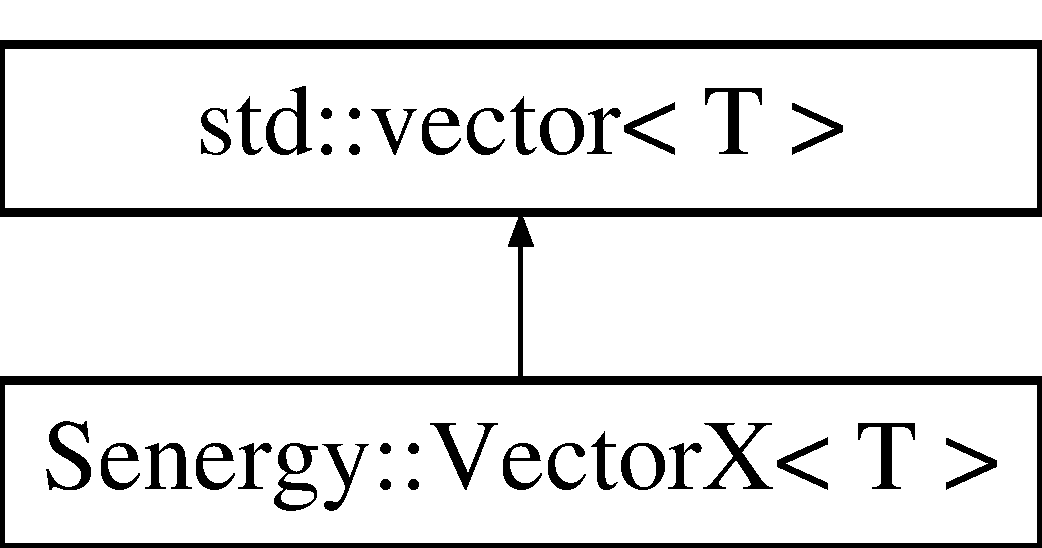
\includegraphics[height=2.000000cm]{class_senergy_1_1_vector_x}
\end{center}
\end{figure}
\subsection*{Public Member Functions}
\begin{DoxyCompactItemize}
\item 
\hyperlink{class_senergy_1_1_vector_x_a99bed6d49a3a93e6a133837330218ee7}{Vector\-X} ()
\begin{DoxyCompactList}\small\item\em Initializes a new, empty vector. \end{DoxyCompactList}\item 
T \hyperlink{class_senergy_1_1_vector_x_a4df34dceed944ef14df649a538d9c1b1}{Add} (T value)
\begin{DoxyCompactList}\small\item\em Adds the specified item to the vector. \end{DoxyCompactList}\end{DoxyCompactItemize}


\subsection{Detailed Description}
\subsubsection*{template$<$class T$>$class Senergy\-::\-Vector\-X$<$ T $>$}

An improvemend upon the standard vector (std\-::vector), but it's interface is more like the rest of \hyperlink{namespace_senergy}{Senergy} (naming). All normal functionality is still available, and switching between \hyperlink{class_senergy_1_1_vector_x}{Vector\-X} and std\-::vector should be painless. 

T The type that the vector will contain.

\begin{DoxyAuthor}{Author}
Swen Kooij (Photonios) 
\end{DoxyAuthor}


Definition at line 40 of file vectorx.\-h.



\subsection{Constructor \& Destructor Documentation}
\hypertarget{class_senergy_1_1_vector_x_a99bed6d49a3a93e6a133837330218ee7}{\index{Senergy\-::\-Vector\-X@{Senergy\-::\-Vector\-X}!Vector\-X@{Vector\-X}}
\index{Vector\-X@{Vector\-X}!Senergy::VectorX@{Senergy\-::\-Vector\-X}}
\subsubsection[{Vector\-X}]{\setlength{\rightskip}{0pt plus 5cm}template$<$class T$>$ {\bf Senergy\-::\-Vector\-X}$<$ T $>$\-::{\bf Vector\-X} (
\begin{DoxyParamCaption}
{}
\end{DoxyParamCaption}
)\hspace{0.3cm}{\ttfamily [inline]}}}\label{class_senergy_1_1_vector_x_a99bed6d49a3a93e6a133837330218ee7}


Initializes a new, empty vector. 



Definition at line 46 of file vectorx.\-h.



\subsection{Member Function Documentation}
\hypertarget{class_senergy_1_1_vector_x_a4df34dceed944ef14df649a538d9c1b1}{\index{Senergy\-::\-Vector\-X@{Senergy\-::\-Vector\-X}!Add@{Add}}
\index{Add@{Add}!Senergy::VectorX@{Senergy\-::\-Vector\-X}}
\subsubsection[{Add}]{\setlength{\rightskip}{0pt plus 5cm}template$<$class T$>$ T {\bf Senergy\-::\-Vector\-X}$<$ T $>$\-::Add (
\begin{DoxyParamCaption}
\item[{T}]{value}
\end{DoxyParamCaption}
)\hspace{0.3cm}{\ttfamily [inline]}}}\label{class_senergy_1_1_vector_x_a4df34dceed944ef14df649a538d9c1b1}


Adds the specified item to the vector. 


\begin{DoxyParams}{Parameters}
{\em value} & The object/value to add to the vector. \\
\hline
\end{DoxyParams}


Definition at line 55 of file vectorx.\-h.



The documentation for this class was generated from the following file\-:\begin{DoxyCompactItemize}
\item 
src/senergy/\hyperlink{vectorx_8h}{vectorx.\-h}\end{DoxyCompactItemize}

\chapter{File Documentation}
\hypertarget{building_8dox}{\section{docs/pages/building.dox File Reference}
\label{building_8dox}\index{docs/pages/building.\-dox@{docs/pages/building.\-dox}}
}

\hypertarget{mainpage_8dox}{\section{docs/pages/mainpage.dox File Reference}
\label{mainpage_8dox}\index{docs/pages/mainpage.\-dox@{docs/pages/mainpage.\-dox}}
}

\hypertarget{references_8dox}{\section{docs/pages/references.dox File Reference}
\label{references_8dox}\index{docs/pages/references.\-dox@{docs/pages/references.\-dox}}
}

\hypertarget{terminology_8dox}{\section{docs/pages/terminology.dox File Reference}
\label{terminology_8dox}\index{docs/pages/terminology.\-dox@{docs/pages/terminology.\-dox}}
}

\hypertarget{bytebuffer_8cpp}{\section{src/bytebuffer.cpp File Reference}
\label{bytebuffer_8cpp}\index{src/bytebuffer.\-cpp@{src/bytebuffer.\-cpp}}
}
{\ttfamily \#include $<$senergy/bytebuffer.\-h$>$}\\*
\subsection*{Namespaces}
\begin{DoxyCompactItemize}
\item 
\hyperlink{namespace_senergy}{Senergy}
\end{DoxyCompactItemize}

\hypertarget{circular__buffer_8cpp}{\section{src/circular\-\_\-buffer.cpp File Reference}
\label{circular__buffer_8cpp}\index{src/circular\-\_\-buffer.\-cpp@{src/circular\-\_\-buffer.\-cpp}}
}
{\ttfamily \#include $<$senergy/circular\-\_\-buffer.\-h$>$}\\*

\hypertarget{convert_8cpp}{\section{src/convert.cpp File Reference}
\label{convert_8cpp}\index{src/convert.\-cpp@{src/convert.\-cpp}}
}
{\ttfamily \#include $<$senergy/convert.\-h$>$}\\*
\subsection*{Namespaces}
\begin{DoxyCompactItemize}
\item 
\hyperlink{namespace_senergy}{Senergy}
\end{DoxyCompactItemize}

\hypertarget{id__factory_8cpp}{\section{src/id\-\_\-factory.cpp File Reference}
\label{id__factory_8cpp}\index{src/id\-\_\-factory.\-cpp@{src/id\-\_\-factory.\-cpp}}
}
{\ttfamily \#include $<$senergy/dns/id\-\_\-factory.\-h$>$}\\*
\subsection*{Namespaces}
\begin{DoxyCompactItemize}
\item 
\hyperlink{namespace_senergy}{Senergy}
\item 
\hyperlink{namespace_senergy_1_1_dns}{Senergy\-::\-Dns}
\end{DoxyCompactItemize}

\hypertarget{main_8cpp}{\section{src/main.cpp File Reference}
\label{main_8cpp}\index{src/main.\-cpp@{src/main.\-cpp}}
}
{\ttfamily \#include $<$iostream$>$}\\*
{\ttfamily \#include $<$senergy/senergy.\-h$>$}\\*
\subsection*{Classes}
\begin{DoxyCompactItemize}
\item 
struct \hyperlink{struct_d_n_s___h_e_a_d_e_r}{D\-N\-S\-\_\-\-H\-E\-A\-D\-E\-R}
\end{DoxyCompactItemize}
\subsection*{Functions}
\begin{DoxyCompactItemize}
\item 
unsigned char $\ast$ \hyperlink{main_8cpp_a1390696935c0b2a9bdebc396feef9688}{Read\-Name} (unsigned char $\ast$reader, unsigned char $\ast$buffer, int $\ast$count)
\item 
int \hyperlink{main_8cpp_a3c04138a5bfe5d72780bb7e82a18e627}{main} (int argc, char $\ast$$\ast$argv)
\end{DoxyCompactItemize}


\subsection{Function Documentation}
\hypertarget{main_8cpp_a3c04138a5bfe5d72780bb7e82a18e627}{\index{main.\-cpp@{main.\-cpp}!main@{main}}
\index{main@{main}!main.cpp@{main.\-cpp}}
\subsubsection[{main}]{\setlength{\rightskip}{0pt plus 5cm}int main (
\begin{DoxyParamCaption}
\item[{int}]{argc, }
\item[{char $\ast$$\ast$}]{argv}
\end{DoxyParamCaption}
)}}\label{main_8cpp_a3c04138a5bfe5d72780bb7e82a18e627}


Definition at line 97 of file main.\-cpp.

\hypertarget{main_8cpp_a1390696935c0b2a9bdebc396feef9688}{\index{main.\-cpp@{main.\-cpp}!Read\-Name@{Read\-Name}}
\index{Read\-Name@{Read\-Name}!main.cpp@{main.\-cpp}}
\subsubsection[{Read\-Name}]{\setlength{\rightskip}{0pt plus 5cm}unsigned char$\ast$ Read\-Name (
\begin{DoxyParamCaption}
\item[{unsigned char $\ast$}]{reader, }
\item[{unsigned char $\ast$}]{buffer, }
\item[{int $\ast$}]{count}
\end{DoxyParamCaption}
)}}\label{main_8cpp_a1390696935c0b2a9bdebc396feef9688}


Definition at line 44 of file main.\-cpp.


\hypertarget{message_8cpp}{\section{src/message.cpp File Reference}
\label{message_8cpp}\index{src/message.\-cpp@{src/message.\-cpp}}
}
{\ttfamily \#include $<$senergy/dns/message.\-h$>$}\\*
\subsection*{Namespaces}
\begin{DoxyCompactItemize}
\item 
\hyperlink{namespace_senergy}{Senergy}
\item 
\hyperlink{namespace_senergy_1_1_dns}{Senergy\-::\-Dns}
\end{DoxyCompactItemize}

\hypertarget{message__header_8cpp}{\section{src/message\-\_\-header.cpp File Reference}
\label{message__header_8cpp}\index{src/message\-\_\-header.\-cpp@{src/message\-\_\-header.\-cpp}}
}
{\ttfamily \#include $<$senergy/dns/message\-\_\-header.\-h$>$}\\*
\subsection*{Namespaces}
\begin{DoxyCompactItemize}
\item 
\hyperlink{namespace_senergy}{Senergy}
\item 
\hyperlink{namespace_senergy_1_1_dns}{Senergy\-::\-Dns}
\end{DoxyCompactItemize}

\hypertarget{message__question_8cpp}{\section{src/message\-\_\-question.cpp File Reference}
\label{message__question_8cpp}\index{src/message\-\_\-question.\-cpp@{src/message\-\_\-question.\-cpp}}
}
{\ttfamily \#include $<$senergy/dns/message\-\_\-question.\-h$>$}\\*
{\ttfamily \#include $<$senergy/convert.\-h$>$}\\*
\subsection*{Namespaces}
\begin{DoxyCompactItemize}
\item 
\hyperlink{namespace_senergy}{Senergy}
\item 
\hyperlink{namespace_senergy_1_1_dns}{Senergy\-::\-Dns}
\end{DoxyCompactItemize}

\hypertarget{print_8cpp}{\section{src/print.cpp File Reference}
\label{print_8cpp}\index{src/print.\-cpp@{src/print.\-cpp}}
}
{\ttfamily \#include $<$senergy/print.\-h$>$}\\*
\subsection*{Namespaces}
\begin{DoxyCompactItemize}
\item 
\hyperlink{namespace_senergy}{Senergy}
\end{DoxyCompactItemize}

\hypertarget{record__ipv4address_8cpp}{\section{src/record\-\_\-ipv4address.cpp File Reference}
\label{record__ipv4address_8cpp}\index{src/record\-\_\-ipv4address.\-cpp@{src/record\-\_\-ipv4address.\-cpp}}
}
{\ttfamily \#include $<$senergy/dns/record\-\_\-ipv4address.\-h$>$}\\*
\subsection*{Namespaces}
\begin{DoxyCompactItemize}
\item 
\hyperlink{namespace_senergy}{Senergy}
\item 
\hyperlink{namespace_senergy_1_1_dns}{Senergy\-::\-Dns}
\item 
\hyperlink{namespace_senergy_1_1_dns_1_1_records}{Senergy\-::\-Dns\-::\-Records}
\end{DoxyCompactItemize}

\hypertarget{requester_8cpp}{\section{src/requester.cpp File Reference}
\label{requester_8cpp}\index{src/requester.\-cpp@{src/requester.\-cpp}}
}
{\ttfamily \#include $<$senergy/dns/requester.\-h$>$}\\*
\subsection*{Namespaces}
\begin{DoxyCompactItemize}
\item 
\hyperlink{namespace_senergy}{Senergy}
\item 
\hyperlink{namespace_senergy_1_1_dns}{Senergy\-::\-Dns}
\end{DoxyCompactItemize}

\hypertarget{resource__record_8cpp}{\section{src/resource\-\_\-record.cpp File Reference}
\label{resource__record_8cpp}\index{src/resource\-\_\-record.\-cpp@{src/resource\-\_\-record.\-cpp}}
}
{\ttfamily \#include $<$senergy/dns/resource\-\_\-record.\-h$>$}\\*
\subsection*{Namespaces}
\begin{DoxyCompactItemize}
\item 
\hyperlink{namespace_senergy}{Senergy}
\item 
\hyperlink{namespace_senergy_1_1_dns}{Senergy\-::\-Dns}
\end{DoxyCompactItemize}

\hypertarget{resource__record__classes_8cpp}{\section{src/resource\-\_\-record\-\_\-classes.cpp File Reference}
\label{resource__record__classes_8cpp}\index{src/resource\-\_\-record\-\_\-classes.\-cpp@{src/resource\-\_\-record\-\_\-classes.\-cpp}}
}
{\ttfamily \#include $<$senergy/dns/resource\-\_\-record\-\_\-classes.\-h$>$}\\*

\hypertarget{resource__record__types_8cpp}{\section{src/resource\-\_\-record\-\_\-types.cpp File Reference}
\label{resource__record__types_8cpp}\index{src/resource\-\_\-record\-\_\-types.\-cpp@{src/resource\-\_\-record\-\_\-types.\-cpp}}
}
{\ttfamily \#include $<$senergy/dns/resource\-\_\-record\-\_\-types.\-h$>$}\\*

\hypertarget{rootnameserver_8cpp}{\section{src/rootnameserver.cpp File Reference}
\label{rootnameserver_8cpp}\index{src/rootnameserver.\-cpp@{src/rootnameserver.\-cpp}}
}
{\ttfamily \#include $<$senergy/dns/rootnameserver.\-h$>$}\\*
\subsection*{Namespaces}
\begin{DoxyCompactItemize}
\item 
\hyperlink{namespace_senergy}{Senergy}
\item 
\hyperlink{namespace_senergy_1_1_dns}{Senergy\-::\-Dns}
\end{DoxyCompactItemize}

\hypertarget{bytebuffer_8h}{\section{src/senergy/bytebuffer.h File Reference}
\label{bytebuffer_8h}\index{src/senergy/bytebuffer.\-h@{src/senergy/bytebuffer.\-h}}
}
{\ttfamily \#include $<$string$>$}\\*
{\ttfamily \#include $<$cstring$>$}\\*
{\ttfamily \#include $<$cstdlib$>$}\\*
{\ttfamily \#include $<$memory$>$}\\*
{\ttfamily \#include $<$senergy/print.\-h$>$}\\*
\subsection*{Classes}
\begin{DoxyCompactItemize}
\item 
class \hyperlink{class_senergy_1_1_byte_buffer}{Senergy\-::\-Byte\-Buffer}
\begin{DoxyCompactList}\small\item\em A dynamiclly sized buffer for binary data. Resizes the underlying buffer when new data is written. Makes it easier to write to buffers that already contain data. \end{DoxyCompactList}\end{DoxyCompactItemize}
\subsection*{Namespaces}
\begin{DoxyCompactItemize}
\item 
\hyperlink{namespace_senergy}{Senergy}
\end{DoxyCompactItemize}
\subsection*{Typedefs}
\begin{DoxyCompactItemize}
\item 
typedef std\-::shared\-\_\-ptr\\*
$<$ Byte\-Buffer $>$ \hyperlink{namespace_senergy_a30f5cfaeb333ffdf2c3332cc590a57ea}{Senergy\-::\-Byte\-Buffer\-Ptr}
\begin{DoxyCompactList}\small\item\em A simple typedef for a shared pointer to a \hyperlink{class_senergy_1_1_byte_buffer}{Byte\-Buffer} instance. \end{DoxyCompactList}\end{DoxyCompactItemize}

\hypertarget{circular__buffer_8h}{\section{src/senergy/circular\-\_\-buffer.h File Reference}
\label{circular__buffer_8h}\index{src/senergy/circular\-\_\-buffer.\-h@{src/senergy/circular\-\_\-buffer.\-h}}
}
{\ttfamily \#include $<$vector$>$}\\*
\subsection*{Classes}
\begin{DoxyCompactItemize}
\item 
class \hyperlink{class_senergy_1_1_circular_buffer}{Senergy\-::\-Circular\-Buffer$<$ T $>$}
\begin{DoxyCompactList}\small\item\em Simple circular buffer which uses a vector, simple circular buffer which should not be used in situations that require efficiency and power. \end{DoxyCompactList}\end{DoxyCompactItemize}
\subsection*{Namespaces}
\begin{DoxyCompactItemize}
\item 
\hyperlink{namespace_senergy}{Senergy}
\end{DoxyCompactItemize}

\hypertarget{convert_8h}{\section{src/senergy/convert.h File Reference}
\label{convert_8h}\index{src/senergy/convert.\-h@{src/senergy/convert.\-h}}
}
{\ttfamily \#include $<$string$>$}\\*
{\ttfamily \#include $<$cstdio$>$}\\*
{\ttfamily \#include $<$cmath$>$}\\*
{\ttfamily \#include $<$ctgmath$>$}\\*
\subsection*{Classes}
\begin{DoxyCompactItemize}
\item 
class \hyperlink{class_senergy_1_1_convert}{Senergy\-::\-Convert}
\begin{DoxyCompactList}\small\item\em A simple conversion class, which simplifies conversion between various native data types. Based on the idea of the '\hyperlink{class_senergy_1_1_convert}{Convert}' class in the .N\-E\-T framework. \end{DoxyCompactList}\end{DoxyCompactItemize}
\subsection*{Namespaces}
\begin{DoxyCompactItemize}
\item 
\hyperlink{namespace_senergy}{Senergy}
\end{DoxyCompactItemize}

\hypertarget{id__factory_8h}{\section{src/senergy/dns/id\-\_\-factory.h File Reference}
\label{id__factory_8h}\index{src/senergy/dns/id\-\_\-factory.\-h@{src/senergy/dns/id\-\_\-factory.\-h}}
}
{\ttfamily \#include $<$stdlib.\-h$>$}\\*
{\ttfamily \#include $<$mutex$>$}\\*
{\ttfamily \#include $<$random$>$}\\*
{\ttfamily \#include $<$senergy/circular\-\_\-buffer.\-h$>$}\\*
\subsection*{Classes}
\begin{DoxyCompactItemize}
\item 
class \hyperlink{class_senergy_1_1_dns_1_1_id_factory}{Senergy\-::\-Dns\-::\-Id\-Factory}
\begin{DoxyCompactList}\small\item\em Static global factory that is used to generate random identifiers for D\-N\-S messages/packets. This is to ensure, each I\-D that is generated is unique. \end{DoxyCompactList}\end{DoxyCompactItemize}
\subsection*{Namespaces}
\begin{DoxyCompactItemize}
\item 
\hyperlink{namespace_senergy}{Senergy}
\item 
\hyperlink{namespace_senergy_1_1_dns}{Senergy\-::\-Dns}
\end{DoxyCompactItemize}

\hypertarget{message_8h}{\section{src/senergy/dns/message.h File Reference}
\label{message_8h}\index{src/senergy/dns/message.\-h@{src/senergy/dns/message.\-h}}
}
{\ttfamily \#include $<$senergy/dns/message\-\_\-header.\-h$>$}\\*
{\ttfamily \#include $<$senergy/dns/message\-\_\-question.\-h$>$}\\*
{\ttfamily \#include $<$senergy/dns/resource\-\_\-record\-\_\-collection.\-h$>$}\\*
{\ttfamily \#include $<$senergy/bytebuffer.\-h$>$}\\*
{\ttfamily \#include $<$senergy/vectorx.\-h$>$}\\*
{\ttfamily \#include $<$algorithm$>$}\\*
{\ttfamily \#include $<$string$>$}\\*
\subsection*{Classes}
\begin{DoxyCompactItemize}
\item 
class \hyperlink{class_senergy_1_1_dns_1_1_message}{Senergy\-::\-Dns\-::\-Message}
\begin{DoxyCompactList}\small\item\em Represents a D\-N\-S packet as described in section 4 of R\-F\-C-\/1035. A D\-N\-S packet is the standard message format that is transmitted and received by D\-N\-S clients and hosts. \end{DoxyCompactList}\end{DoxyCompactItemize}
\subsection*{Namespaces}
\begin{DoxyCompactItemize}
\item 
\hyperlink{namespace_senergy}{Senergy}
\item 
\hyperlink{namespace_senergy_1_1_dns}{Senergy\-::\-Dns}
\end{DoxyCompactItemize}

\hypertarget{message__header_8h}{\section{src/senergy/dns/message\-\_\-header.h File Reference}
\label{message__header_8h}\index{src/senergy/dns/message\-\_\-header.\-h@{src/senergy/dns/message\-\_\-header.\-h}}
}
{\ttfamily \#include $<$senergy/bytebuffer.\-h$>$}\\*
\subsection*{Classes}
\begin{DoxyCompactItemize}
\item 
struct \hyperlink{struct_senergy_1_1_dns_1_1_message_header_fields}{Senergy\-::\-Dns\-::\-Message\-Header\-Fields}
\begin{DoxyCompactList}\small\item\em Defines the fields within a D\-N\-S packet header, as described in section 4.\-1 of R\-F\-C-\/1035. This data structure is used as the \char`\"{}\-Fields\char`\"{} member/property of the \hyperlink{class_senergy_1_1_dns_1_1_message_header}{Message\-Header} class, and serves as the container of the actual data. \end{DoxyCompactList}\item 
class \hyperlink{class_senergy_1_1_dns_1_1_message_header}{Senergy\-::\-Dns\-::\-Message\-Header}
\begin{DoxyCompactList}\small\item\em Defines the header of a D\-N\-S packet, as described in section 4.\-1 of R\-F\-C-\/1035. All D\-N\-S messages start with this header. \end{DoxyCompactList}\end{DoxyCompactItemize}
\subsection*{Namespaces}
\begin{DoxyCompactItemize}
\item 
\hyperlink{namespace_senergy}{Senergy}
\item 
\hyperlink{namespace_senergy_1_1_dns}{Senergy\-::\-Dns}
\end{DoxyCompactItemize}

\hypertarget{message__question_8h}{\section{src/senergy/dns/message\-\_\-question.h File Reference}
\label{message__question_8h}\index{src/senergy/dns/message\-\_\-question.\-h@{src/senergy/dns/message\-\_\-question.\-h}}
}
{\ttfamily \#include $<$senergy/bytebuffer.\-h$>$}\\*
{\ttfamily \#include $<$senergy/convert.\-h$>$}\\*
{\ttfamily \#include $<$senergy/vectorx.\-h$>$}\\*
{\ttfamily \#include $<$senergy/dns/resource\-\_\-record\-\_\-types.\-h$>$}\\*
{\ttfamily \#include $<$senergy/dns/resource\-\_\-record\-\_\-classes.\-h$>$}\\*
{\ttfamily \#include $<$senergy/dns/utils.\-h$>$}\\*
{\ttfamily \#include $<$cstdio$>$}\\*
{\ttfamily \#include $<$cctype$>$}\\*
{\ttfamily \#include $<$string$>$}\\*
{\ttfamily \#include $<$vector$>$}\\*
{\ttfamily \#include $<$memory$>$}\\*
{\ttfamily \#include $<$arpa/inet.\-h$>$}\\*
\subsection*{Classes}
\begin{DoxyCompactItemize}
\item 
class \hyperlink{class_senergy_1_1_dns_1_1_message_question}{Senergy\-::\-Dns\-::\-Message\-Question}
\begin{DoxyCompactList}\small\item\em Represents a D\-N\-S question, as defined in section 4.\-1.\-2 of R\-F\-C-\/1035. A D\-N\-S question is usually transmitted by a D\-N\-S client, asking to lookup the I\-P address of a host name. \end{DoxyCompactList}\end{DoxyCompactItemize}
\subsection*{Namespaces}
\begin{DoxyCompactItemize}
\item 
\hyperlink{namespace_senergy}{Senergy}
\item 
\hyperlink{namespace_senergy_1_1_dns}{Senergy\-::\-Dns}
\end{DoxyCompactItemize}
\subsection*{Macros}
\begin{DoxyCompactItemize}
\item 
\#define \hyperlink{message__question_8h_a4b780ef30c07c3c31b79d838bc443687}{Message\-Question\-Ptr}~std\-::shared\-\_\-ptr$<$Message\-Question$>$
\item 
\#define \hyperlink{message__question_8h_aa505746d3e0a330ca99da6969d9d1c5a}{Message\-Question\-Ptr\-Vector}~Vector\-X$<$\hyperlink{message__question_8h_a4b780ef30c07c3c31b79d838bc443687}{Message\-Question\-Ptr}$>$
\end{DoxyCompactItemize}


\subsection{Macro Definition Documentation}
\hypertarget{message__question_8h_a4b780ef30c07c3c31b79d838bc443687}{\index{message\-\_\-question.\-h@{message\-\_\-question.\-h}!Message\-Question\-Ptr@{Message\-Question\-Ptr}}
\index{Message\-Question\-Ptr@{Message\-Question\-Ptr}!message_question.h@{message\-\_\-question.\-h}}
\subsubsection[{Message\-Question\-Ptr}]{\setlength{\rightskip}{0pt plus 5cm}\#define Message\-Question\-Ptr~std\-::shared\-\_\-ptr$<$Message\-Question$>$}}\label{message__question_8h_a4b780ef30c07c3c31b79d838bc443687}


Definition at line 43 of file message\-\_\-question.\-h.

\hypertarget{message__question_8h_aa505746d3e0a330ca99da6969d9d1c5a}{\index{message\-\_\-question.\-h@{message\-\_\-question.\-h}!Message\-Question\-Ptr\-Vector@{Message\-Question\-Ptr\-Vector}}
\index{Message\-Question\-Ptr\-Vector@{Message\-Question\-Ptr\-Vector}!message_question.h@{message\-\_\-question.\-h}}
\subsubsection[{Message\-Question\-Ptr\-Vector}]{\setlength{\rightskip}{0pt plus 5cm}\#define Message\-Question\-Ptr\-Vector~Vector\-X$<${\bf Message\-Question\-Ptr}$>$}}\label{message__question_8h_aa505746d3e0a330ca99da6969d9d1c5a}


Definition at line 44 of file message\-\_\-question.\-h.


\hypertarget{record__ipv4address_8h}{\section{src/senergy/dns/record\-\_\-ipv4address.h File Reference}
\label{record__ipv4address_8h}\index{src/senergy/dns/record\-\_\-ipv4address.\-h@{src/senergy/dns/record\-\_\-ipv4address.\-h}}
}
{\ttfamily \#include $<$string$>$}\\*
{\ttfamily \#include $<$senergy/dns/resource\-\_\-record\-\_\-types.\-h$>$}\\*
{\ttfamily \#include $<$senergy/dns/resource\-\_\-record\-\_\-classes.\-h$>$}\\*
{\ttfamily \#include $<$senergy/dns/message\-\_\-header.\-h$>$}\\*
{\ttfamily \#include $<$senergy/dns/resource\-\_\-record.\-h$>$}\\*
{\ttfamily \#include $<$senergy/socket.\-h$>$}\\*
{\ttfamily \#include $<$senergy/vectorx.\-h$>$}\\*
\subsection*{Classes}
\begin{DoxyCompactItemize}
\item 
class \hyperlink{class_senergy_1_1_dns_1_1_records_1_1_i_p_v4_address}{Senergy\-::\-Dns\-::\-Records\-::\-I\-P\-V4\-Address}
\begin{DoxyCompactList}\small\item\em An address record, contains the answer to a lookup. Contains a I\-P\-V4 I\-P address, the response to a question, to lookup a hostname/domain name. This is part of a resource record, and the actual data is stored in the last field of a recource record (R\-D\-A\-T\-E). See the Resource\-Class and section 3.\-4.\-1 of R\-F\-C 1035 for more information. \end{DoxyCompactList}\end{DoxyCompactItemize}
\subsection*{Namespaces}
\begin{DoxyCompactItemize}
\item 
\hyperlink{namespace_senergy}{Senergy}
\item 
\hyperlink{namespace_senergy_1_1_dns}{Senergy\-::\-Dns}
\item 
\hyperlink{namespace_senergy_1_1_dns_1_1_records}{Senergy\-::\-Dns\-::\-Records}
\end{DoxyCompactItemize}
\subsection*{Typedefs}
\begin{DoxyCompactItemize}
\item 
typedef std\-::shared\-\_\-ptr\\*
$<$ I\-P\-V4\-Address $>$ \hyperlink{namespace_senergy_1_1_dns_1_1_records_a3f0d02fcd6381aee3fab67589ac0890c}{Senergy\-::\-Dns\-::\-Records\-::\-I\-P\-V4\-Address\-Ptr}
\begin{DoxyCompactList}\small\item\em A shared pointer to a \hyperlink{class_senergy_1_1_dns_1_1_records_1_1_i_p_v4_address}{I\-P\-V4\-Address} instance. \end{DoxyCompactList}\item 
typedef Vector\-X$<$ I\-P\-V4\-Address\-Ptr $>$ \hyperlink{namespace_senergy_1_1_dns_1_1_records_a5b9115e6124c4999bbb000e69cfe5d2c}{Senergy\-::\-Dns\-::\-Records\-::\-I\-P\-V4\-Address\-Ptr\-Vector}
\begin{DoxyCompactList}\small\item\em A vector of shared pointers to \hyperlink{class_senergy_1_1_dns_1_1_records_1_1_i_p_v4_address}{I\-P\-V4\-Address} instances. \end{DoxyCompactList}\end{DoxyCompactItemize}

\hypertarget{requester_8h}{\section{src/senergy/dns/requester.h File Reference}
\label{requester_8h}\index{src/senergy/dns/requester.\-h@{src/senergy/dns/requester.\-h}}
}
{\ttfamily \#include $<$senergy/bytebuffer.\-h$>$}\\*
{\ttfamily \#include $<$senergy/socket.\-h$>$}\\*
{\ttfamily \#include $<$senergy/vectorx.\-h$>$}\\*
{\ttfamily \#include $<$senergy/types.\-h$>$}\\*
{\ttfamily \#include $<$senergy/dns/message.\-h$>$}\\*
{\ttfamily \#include $<$senergy/dns/resource\-\_\-record\-\_\-types.\-h$>$}\\*
\subsection*{Classes}
\begin{DoxyCompactItemize}
\item 
class \hyperlink{class_senergy_1_1_dns_1_1_requester}{Senergy\-::\-Dns\-::\-Requester}
\begin{DoxyCompactList}\small\item\em Allows querying remote D\-N\-S servers, wraps sending and receiving D\-N\-S messages. \end{DoxyCompactList}\end{DoxyCompactItemize}
\subsection*{Namespaces}
\begin{DoxyCompactItemize}
\item 
\hyperlink{namespace_senergy}{Senergy}
\item 
\hyperlink{namespace_senergy_1_1_dns}{Senergy\-::\-Dns}
\end{DoxyCompactItemize}

\hypertarget{resource__record_8h}{\section{src/senergy/dns/resource\-\_\-record.h File Reference}
\label{resource__record_8h}\index{src/senergy/dns/resource\-\_\-record.\-h@{src/senergy/dns/resource\-\_\-record.\-h}}
}
{\ttfamily \#include $<$string$>$}\\*
{\ttfamily \#include $<$memory$>$}\\*
{\ttfamily \#include $<$senergy/dns/resource\-\_\-record\-\_\-types.\-h$>$}\\*
{\ttfamily \#include $<$senergy/dns/resource\-\_\-record\-\_\-classes.\-h$>$}\\*
{\ttfamily \#include $<$senergy/vectorx.\-h$>$}\\*
{\ttfamily \#include $<$senergy/dns/utils.\-h$>$}\\*
{\ttfamily \#include $<$senergy/bytebuffer.\-h$>$}\\*
\subsection*{Classes}
\begin{DoxyCompactItemize}
\item 
class \hyperlink{class_senergy_1_1_dns_1_1_resource_record}{Senergy\-::\-Dns\-::\-Resource\-Record}
\begin{DoxyCompactList}\small\item\em Defines a D\-N\-S Resource Record, as defined in R\-F\-C 1035, section 4.\-1.\-3. A D\-N\-S Recource record can appear both in the answer, authority and additional section of a D\-N\-S packet/message. \end{DoxyCompactList}\end{DoxyCompactItemize}
\subsection*{Namespaces}
\begin{DoxyCompactItemize}
\item 
\hyperlink{namespace_senergy}{Senergy}
\item 
\hyperlink{namespace_senergy_1_1_dns}{Senergy\-::\-Dns}
\end{DoxyCompactItemize}
\subsection*{Typedefs}
\begin{DoxyCompactItemize}
\item 
typedef std\-::shared\-\_\-ptr\\*
$<$ Resource\-Record $>$ \hyperlink{namespace_senergy_1_1_dns_a1fa04259a07ce7a270e09288aa456ffd}{Senergy\-::\-Dns\-::\-Resource\-Record\-Ptr}
\begin{DoxyCompactList}\small\item\em A shared pointer to an instance of the \hyperlink{class_senergy_1_1_dns_1_1_resource_record}{Resource\-Record} class. \end{DoxyCompactList}\item 
typedef Vector\-X\\*
$<$ Resource\-Record\-Ptr $>$ \hyperlink{namespace_senergy_1_1_dns_ad5ef448b2b508ce86c6ed91dccc10d3e}{Senergy\-::\-Dns\-::\-Resource\-Record\-Ptr\-Vector}
\begin{DoxyCompactList}\small\item\em A vector of shared pointers to \hyperlink{class_senergy_1_1_dns_1_1_resource_record}{Resource\-Record} class instances. \end{DoxyCompactList}\end{DoxyCompactItemize}

\hypertarget{resource__record__classes_8h}{\section{src/senergy/dns/resource\-\_\-record\-\_\-classes.h File Reference}
\label{resource__record__classes_8h}\index{src/senergy/dns/resource\-\_\-record\-\_\-classes.\-h@{src/senergy/dns/resource\-\_\-record\-\_\-classes.\-h}}
}
\subsection*{Namespaces}
\begin{DoxyCompactItemize}
\item 
\hyperlink{namespace_senergy}{Senergy}
\item 
\hyperlink{namespace_senergy_1_1_dns}{Senergy\-::\-Dns}
\end{DoxyCompactItemize}
\subsection*{Enumerations}
\begin{DoxyCompactItemize}
\item 
enum \hyperlink{namespace_senergy_1_1_dns_a953f153bc411213d621d00c1e1b3eb9d}{Senergy\-::\-Dns\-::\-Resource\-Record\-Class} \-: unsigned short \{ \\*
\hyperlink{namespace_senergy_1_1_dns_a953f153bc411213d621d00c1e1b3eb9da942d4e37dd5607ab68e54755540d4a47}{Senergy\-::\-Dns\-::\-Resource\-Record\-Class\-::\-Reserved} = 0, 
\hyperlink{namespace_senergy_1_1_dns_a953f153bc411213d621d00c1e1b3eb9dac8205c7636e728d448c2774e6a4a944b}{Senergy\-::\-Dns\-::\-Resource\-Record\-Class\-::\-Internet} = 1, 
\hyperlink{namespace_senergy_1_1_dns_a953f153bc411213d621d00c1e1b3eb9da7e8214916782021125d0afd9d9d9ee66}{Senergy\-::\-Dns\-::\-Resource\-Record\-Class\-::\-Chaos} = 2, 
\hyperlink{namespace_senergy_1_1_dns_a953f153bc411213d621d00c1e1b3eb9da04e26d2a6e2432efc191fd0b9d9f0c9c}{Senergy\-::\-Dns\-::\-Resource\-Record\-Class\-::\-Hesiod} = 3, 
\\*
\hyperlink{namespace_senergy_1_1_dns_a953f153bc411213d621d00c1e1b3eb9da6adf97f83acf6453d4a6a4b1070f3754}{Senergy\-::\-Dns\-::\-Resource\-Record\-Class\-::\-None} = 254, 
\hyperlink{namespace_senergy_1_1_dns_a953f153bc411213d621d00c1e1b3eb9daed36a1ef76a59ee3f15180e0441188ad}{Senergy\-::\-Dns\-::\-Resource\-Record\-Class\-::\-Any} = 255
 \}
\begin{DoxyCompactList}\small\item\em An enumuration of all possible resource record classes (R\-R) as defined in R\-F\-C-\/1035. None of them except 'Internet' are really used. \end{DoxyCompactList}\end{DoxyCompactItemize}

\hypertarget{resource__record__types_8h}{\section{src/senergy/dns/resource\-\_\-record\-\_\-types.h File Reference}
\label{resource__record__types_8h}\index{src/senergy/dns/resource\-\_\-record\-\_\-types.\-h@{src/senergy/dns/resource\-\_\-record\-\_\-types.\-h}}
}
\subsection*{Namespaces}
\begin{DoxyCompactItemize}
\item 
\hyperlink{namespace_senergy}{Senergy}
\item 
\hyperlink{namespace_senergy_1_1_dns}{Senergy\-::\-Dns}
\end{DoxyCompactItemize}
\subsection*{Enumerations}
\begin{DoxyCompactItemize}
\item 
enum \hyperlink{namespace_senergy_1_1_dns_a590bfd748c955364770f5ce358d9dfe0}{Senergy\-::\-Dns\-::\-Resource\-Record\-Type} \-: unsigned short \{ \\*
\hyperlink{namespace_senergy_1_1_dns_a590bfd748c955364770f5ce358d9dfe0a7fc56270e7a70fa81a5935b72eacbe29}{Senergy\-::\-Dns\-::\-Resource\-Record\-Type\-::\-A} = 1, 
\hyperlink{namespace_senergy_1_1_dns_a590bfd748c955364770f5ce358d9dfe0a53c8d15a175221d2127083e66a8cc937}{Senergy\-::\-Dns\-::\-Resource\-Record\-Type\-::\-N\-S} = 2, 
\hyperlink{namespace_senergy_1_1_dns_a590bfd748c955364770f5ce358d9dfe0a7dc10e66da5549d351765bd940b81be9}{Senergy\-::\-Dns\-::\-Resource\-Record\-Type\-::\-M\-D} = 3, 
\hyperlink{namespace_senergy_1_1_dns_a590bfd748c955364770f5ce358d9dfe0a12c578c9f48dd6727464670d5daa0f9c}{Senergy\-::\-Dns\-::\-Resource\-Record\-Type\-::\-M\-F} = 4, 
\\*
\hyperlink{namespace_senergy_1_1_dns_a590bfd748c955364770f5ce358d9dfe0aadc4bfdb0829dae99e3699393e3fbaa4}{Senergy\-::\-Dns\-::\-Resource\-Record\-Type\-::\-C\-N\-A\-M\-E} = 5, 
\hyperlink{namespace_senergy_1_1_dns_a590bfd748c955364770f5ce358d9dfe0abe5a791366c5f2810d7dd6132dc0f06c}{Senergy\-::\-Dns\-::\-Resource\-Record\-Type\-::\-S\-O\-A} = 6, 
\hyperlink{namespace_senergy_1_1_dns_a590bfd748c955364770f5ce358d9dfe0a8d8fcc1abd550c5f25dbfaa57d59cb67}{Senergy\-::\-Dns\-::\-Resource\-Record\-Type\-::\-M\-B} = 7, 
\hyperlink{namespace_senergy_1_1_dns_a590bfd748c955364770f5ce358d9dfe0aba2a034f4d913f87fe07cad29368d114}{Senergy\-::\-Dns\-::\-Resource\-Record\-Type\-::\-M\-G} = 8, 
\\*
\hyperlink{namespace_senergy_1_1_dns_a590bfd748c955364770f5ce358d9dfe0ad5c44258d51659f96279c470ce8185dc}{Senergy\-::\-Dns\-::\-Resource\-Record\-Type\-::\-M\-R} = 9, 
\hyperlink{namespace_senergy_1_1_dns_a590bfd748c955364770f5ce358d9dfe0a890f5fe6581170eeff26bec1c1e6a023}{Senergy\-::\-Dns\-::\-Resource\-Record\-Type\-::\-N\-U\-L} = 10, 
\hyperlink{namespace_senergy_1_1_dns_a590bfd748c955364770f5ce358d9dfe0aeed02d24534183b7a268008603930b67}{Senergy\-::\-Dns\-::\-Resource\-Record\-Type\-::\-W\-K\-S} = 11, 
\hyperlink{namespace_senergy_1_1_dns_a590bfd748c955364770f5ce358d9dfe0accf95d5d6208e6821c61433d43848f16}{Senergy\-::\-Dns\-::\-Resource\-Record\-Type\-::\-P\-T\-R} = 12, 
\\*
\hyperlink{namespace_senergy_1_1_dns_a590bfd748c955364770f5ce358d9dfe0a6039bc6fb2965fe1e923383f3c3ac936}{Senergy\-::\-Dns\-::\-Resource\-Record\-Type\-::\-H\-I\-N\-F\-O} = 13, 
\hyperlink{namespace_senergy_1_1_dns_a590bfd748c955364770f5ce358d9dfe0adfb31d06b1b1f36e6a6ddfe0f94b33da}{Senergy\-::\-Dns\-::\-Resource\-Record\-Type\-::\-M\-I\-N\-F\-O} = 14, 
\hyperlink{namespace_senergy_1_1_dns_a590bfd748c955364770f5ce358d9dfe0a0b98720dcb2cc6fd60358a45dfbc5b87}{Senergy\-::\-Dns\-::\-Resource\-Record\-Type\-::\-M\-X} = 15, 
\hyperlink{namespace_senergy_1_1_dns_a590bfd748c955364770f5ce358d9dfe0a5956a437e724cdfc8b1c70dc7bdeebcb}{Senergy\-::\-Dns\-::\-Resource\-Record\-Type\-::\-T\-X\-T} = 16, 
\\*
\hyperlink{namespace_senergy_1_1_dns_a590bfd748c955364770f5ce358d9dfe0ac4cb0a6bcf9b947b0e647a11ebfacefa}{Senergy\-::\-Dns\-::\-Resource\-Record\-Type\-::\-R\-P} = 17, 
\hyperlink{namespace_senergy_1_1_dns_a590bfd748c955364770f5ce358d9dfe0ab9e4ee544eaa7fe99267355742f7a03e}{Senergy\-::\-Dns\-::\-Resource\-Record\-Type\-::\-A\-F\-S\-D\-B} = 18, 
\hyperlink{namespace_senergy_1_1_dns_a590bfd748c955364770f5ce358d9dfe0ab9f72c6f03e2177e0ea0f3f31ba05da1}{Senergy\-::\-Dns\-::\-Resource\-Record\-Type\-::\-X25} = 19, 
\hyperlink{namespace_senergy_1_1_dns_a590bfd748c955364770f5ce358d9dfe0a6b76a4f6461388db72ddf5cc41979c4b}{Senergy\-::\-Dns\-::\-Resource\-Record\-Type\-::\-I\-S\-D\-N} = 20, 
\\*
\hyperlink{namespace_senergy_1_1_dns_a590bfd748c955364770f5ce358d9dfe0a705610ed3e5ec724f5cb0d76a5fd3aa1}{Senergy\-::\-Dns\-::\-Resource\-Record\-Type\-::\-R\-T} = 21, 
\hyperlink{namespace_senergy_1_1_dns_a590bfd748c955364770f5ce358d9dfe0ab1749646110d92e1818f7f7cf24d374e}{Senergy\-::\-Dns\-::\-Resource\-Record\-Type\-::\-N\-S\-A\-P} = 22, 
\hyperlink{namespace_senergy_1_1_dns_a590bfd748c955364770f5ce358d9dfe0ae71f755427c9351f13e0b14103a8a549}{Senergy\-::\-Dns\-::\-Resource\-Record\-Type\-::\-N\-S\-A\-P\-\_\-\-P\-T\-R} = 23, 
\hyperlink{namespace_senergy_1_1_dns_a590bfd748c955364770f5ce358d9dfe0a8e40932558a1eaaf985335ab7154d6dc}{Senergy\-::\-Dns\-::\-Resource\-Record\-Type\-::\-S\-I\-G} = 24, 
\\*
\hyperlink{namespace_senergy_1_1_dns_a590bfd748c955364770f5ce358d9dfe0a3b5949e0c26b87767a4752a276de9570}{Senergy\-::\-Dns\-::\-Resource\-Record\-Type\-::\-K\-E\-Y} = 25, 
\hyperlink{namespace_senergy_1_1_dns_a590bfd748c955364770f5ce358d9dfe0a87e6c078833a3c35b65067a50c936b37}{Senergy\-::\-Dns\-::\-Resource\-Record\-Type\-::\-P\-X} = 26, 
\hyperlink{namespace_senergy_1_1_dns_a590bfd748c955364770f5ce358d9dfe0a7fa7750863127fa3f9f1255b582ac34d}{Senergy\-::\-Dns\-::\-Resource\-Record\-Type\-::\-G\-P\-O\-S} = 27, 
\hyperlink{namespace_senergy_1_1_dns_a590bfd748c955364770f5ce358d9dfe0a098890dde069e9abad63f19a0d9e1f32}{Senergy\-::\-Dns\-::\-Resource\-Record\-Type\-::\-A\-A\-A\-A} = 28, 
\\*
\hyperlink{namespace_senergy_1_1_dns_a590bfd748c955364770f5ce358d9dfe0a7982b1597f92456d71b333fe2aead996}{Senergy\-::\-Dns\-::\-Resource\-Record\-Type\-::\-L\-O\-C} = 29, 
\hyperlink{namespace_senergy_1_1_dns_a590bfd748c955364770f5ce358d9dfe0a3f15fada7994f98f3bc6207bed01c16b}{Senergy\-::\-Dns\-::\-Resource\-Record\-Type\-::\-N\-X\-T} = 30, 
\hyperlink{namespace_senergy_1_1_dns_a590bfd748c955364770f5ce358d9dfe0a02cf6cb778382bf4014cc10c4c15b449}{Senergy\-::\-Dns\-::\-Resource\-Record\-Type\-::\-E\-I\-D} = 31, 
\hyperlink{namespace_senergy_1_1_dns_a590bfd748c955364770f5ce358d9dfe0a1ffe19e6ac60395518851cb93ca2e1cf}{Senergy\-::\-Dns\-::\-Resource\-Record\-Type\-::\-N\-I\-M\-L\-O\-C} = 32, 
\\*
\hyperlink{namespace_senergy_1_1_dns_a590bfd748c955364770f5ce358d9dfe0ab71ecf0b186ac1b938e15483f792b7db}{Senergy\-::\-Dns\-::\-Resource\-Record\-Type\-::\-S\-R\-V} = 33, 
\hyperlink{namespace_senergy_1_1_dns_a590bfd748c955364770f5ce358d9dfe0a130eec8777bec09e591885428f2ffb75}{Senergy\-::\-Dns\-::\-Resource\-Record\-Type\-::\-A\-T\-M\-A} = 34, 
\hyperlink{namespace_senergy_1_1_dns_a590bfd748c955364770f5ce358d9dfe0a9bf4e5a83e8c043c90b39c0d1c6a1587}{Senergy\-::\-Dns\-::\-Resource\-Record\-Type\-::\-N\-A\-P\-T\-R} = 35, 
\hyperlink{namespace_senergy_1_1_dns_a590bfd748c955364770f5ce358d9dfe0a33ac0876e2026575dc3b41a0b74c3015}{Senergy\-::\-Dns\-::\-Resource\-Record\-Type\-::\-K\-X} = 36, 
\\*
\hyperlink{namespace_senergy_1_1_dns_a590bfd748c955364770f5ce358d9dfe0a5d2cfab83ed6e86a4812690790dc7ad5}{Senergy\-::\-Dns\-::\-Resource\-Record\-Type\-::\-C\-E\-R\-T} = 37, 
\hyperlink{namespace_senergy_1_1_dns_a590bfd748c955364770f5ce358d9dfe0a0b3d5609ee81e50809b7351e848e4698}{Senergy\-::\-Dns\-::\-Resource\-Record\-Type\-::\-A6} = 38, 
\hyperlink{namespace_senergy_1_1_dns_a590bfd748c955364770f5ce358d9dfe0a78e5dce13f93104bcc1c380f63d7ac17}{Senergy\-::\-Dns\-::\-Resource\-Record\-Type\-::\-D\-N\-A\-M\-E} = 39, 
\hyperlink{namespace_senergy_1_1_dns_a590bfd748c955364770f5ce358d9dfe0a6091f77137cf4570917f3f4d30585bb1}{Senergy\-::\-Dns\-::\-Resource\-Record\-Type\-::\-S\-I\-N\-K} = 40, 
\\*
\hyperlink{namespace_senergy_1_1_dns_a590bfd748c955364770f5ce358d9dfe0ad64669882d28591f1a0fe0926f80e751}{Senergy\-::\-Dns\-::\-Resource\-Record\-Type\-::\-O\-P\-T} = 41, 
\hyperlink{namespace_senergy_1_1_dns_a590bfd748c955364770f5ce358d9dfe0acd5451fbbc151dc5f8020fb1bbc9ef86}{Senergy\-::\-Dns\-::\-Resource\-Record\-Type\-::\-A\-P\-L} = 42, 
\hyperlink{namespace_senergy_1_1_dns_a590bfd748c955364770f5ce358d9dfe0a47b79bd259e22596ffc4be2ffbbe5c5a}{Senergy\-::\-Dns\-::\-Resource\-Record\-Type\-::\-D\-S} = 43, 
\hyperlink{namespace_senergy_1_1_dns_a590bfd748c955364770f5ce358d9dfe0af228c42396e41cfc2c31c9ee79c50f39}{Senergy\-::\-Dns\-::\-Resource\-Record\-Type\-::\-S\-S\-H\-F\-P} = 44, 
\\*
\hyperlink{namespace_senergy_1_1_dns_a590bfd748c955364770f5ce358d9dfe0a2b356a14948fa1c2a2ef3c14355c83ea}{Senergy\-::\-Dns\-::\-Resource\-Record\-Type\-::\-I\-P\-S\-E\-C\-K\-E\-Y} = 45, 
\hyperlink{namespace_senergy_1_1_dns_a590bfd748c955364770f5ce358d9dfe0acedf979874cc1ac262a7a836f504a9a3}{Senergy\-::\-Dns\-::\-Resource\-Record\-Type\-::\-R\-R\-S\-I\-G} = 46, 
\hyperlink{namespace_senergy_1_1_dns_a590bfd748c955364770f5ce358d9dfe0a6ac9d5292ffcb6323409509895e59c6a}{Senergy\-::\-Dns\-::\-Resource\-Record\-Type\-::\-N\-S\-E\-C} = 47, 
\hyperlink{namespace_senergy_1_1_dns_a590bfd748c955364770f5ce358d9dfe0a548deb43a9afe4abcde34a605eb44700}{Senergy\-::\-Dns\-::\-Resource\-Record\-Type\-::\-D\-N\-S\-K\-E\-Y} = 48, 
\\*
\hyperlink{namespace_senergy_1_1_dns_a590bfd748c955364770f5ce358d9dfe0a6e70731664048d83678c263374c8dd35}{Senergy\-::\-Dns\-::\-Resource\-Record\-Type\-::\-D\-H\-C\-I\-D} = 49, 
\hyperlink{namespace_senergy_1_1_dns_a590bfd748c955364770f5ce358d9dfe0aa573cb9749bec7cdc7c1689504db06fa}{Senergy\-::\-Dns\-::\-Resource\-Record\-Type\-::\-N\-S\-E\-C3} = 50, 
\hyperlink{namespace_senergy_1_1_dns_a590bfd748c955364770f5ce358d9dfe0ac31c935076390d6c1f649299c706b21a}{Senergy\-::\-Dns\-::\-Resource\-Record\-Type\-::\-N\-S\-E\-C3\-P\-A\-R\-A\-M} = 51, 
\hyperlink{namespace_senergy_1_1_dns_a590bfd748c955364770f5ce358d9dfe0a2528196793228f3ed012ef32a973842d}{Senergy\-::\-Dns\-::\-Resource\-Record\-Type\-::\-T\-L\-S\-A} = 52, 
\\*
\hyperlink{namespace_senergy_1_1_dns_a590bfd748c955364770f5ce358d9dfe0a5e4576beae2ab86d6ad1b8b1700d2e11}{Senergy\-::\-Dns\-::\-Resource\-Record\-Type\-::\-H\-I\-P} = 55, 
\hyperlink{namespace_senergy_1_1_dns_a590bfd748c955364770f5ce358d9dfe0af2c8bdba2e1534ec4f29d0d7fd637976}{Senergy\-::\-Dns\-::\-Resource\-Record\-Type\-::\-N\-F\-I\-N\-O} = 56, 
\hyperlink{namespace_senergy_1_1_dns_a590bfd748c955364770f5ce358d9dfe0aa0c7a61ee259167ff4eb02668a90798e}{Senergy\-::\-Dns\-::\-Resource\-Record\-Type\-::\-R\-K\-E\-Y} = 57, 
\hyperlink{namespace_senergy_1_1_dns_a590bfd748c955364770f5ce358d9dfe0aae5740157bf2828808b460ef253c6d64}{Senergy\-::\-Dns\-::\-Resource\-Record\-Type\-::\-T\-A\-L\-I\-N\-K} = 58, 
\\*
\hyperlink{namespace_senergy_1_1_dns_a590bfd748c955364770f5ce358d9dfe0ab1da7839edd4969a1aaa4435721a149c}{Senergy\-::\-Dns\-::\-Resource\-Record\-Type\-::\-C\-D\-S} = 59, 
\hyperlink{namespace_senergy_1_1_dns_a590bfd748c955364770f5ce358d9dfe0ab4efb35349e5d93905531be07dbacd6d}{Senergy\-::\-Dns\-::\-Resource\-Record\-Type\-::\-S\-P\-F} = 99, 
\hyperlink{namespace_senergy_1_1_dns_a590bfd748c955364770f5ce358d9dfe0ae9d3d23146a9fbf510b755d3356199b4}{Senergy\-::\-Dns\-::\-Resource\-Record\-Type\-::\-U\-I\-N\-F\-O} = 100, 
\hyperlink{namespace_senergy_1_1_dns_a590bfd748c955364770f5ce358d9dfe0ae7d22294bdcb7133967c3548ece982e5}{Senergy\-::\-Dns\-::\-Resource\-Record\-Type\-::\-U\-I\-D} = 101, 
\\*
\hyperlink{namespace_senergy_1_1_dns_a590bfd748c955364770f5ce358d9dfe0a7af9d03ef884836d52bd6c23c4fc2f79}{Senergy\-::\-Dns\-::\-Resource\-Record\-Type\-::\-G\-I\-D} = 102, 
\hyperlink{namespace_senergy_1_1_dns_a590bfd748c955364770f5ce358d9dfe0a2f03cf10116568e1dbf5263143cffaec}{Senergy\-::\-Dns\-::\-Resource\-Record\-Type\-::\-U\-N\-S\-P\-E\-C} = 103, 
\hyperlink{namespace_senergy_1_1_dns_a590bfd748c955364770f5ce358d9dfe0ab0db97f062879a0e0cd0788528386743}{Senergy\-::\-Dns\-::\-Resource\-Record\-Type\-::\-N\-I\-D} = 104, 
\hyperlink{namespace_senergy_1_1_dns_a590bfd748c955364770f5ce358d9dfe0a3b80517688b93186611e64fe9268fca7}{Senergy\-::\-Dns\-::\-Resource\-Record\-Type\-::\-L32} = 105, 
\\*
\hyperlink{namespace_senergy_1_1_dns_a590bfd748c955364770f5ce358d9dfe0a036a76b97b96b5d46742bb4bcd2ff24d}{Senergy\-::\-Dns\-::\-Resource\-Record\-Type\-::\-L64} = 106, 
\hyperlink{namespace_senergy_1_1_dns_a590bfd748c955364770f5ce358d9dfe0a233724c5adf28da47784390134db3c66}{Senergy\-::\-Dns\-::\-Resource\-Record\-Type\-::\-L\-P} = 107, 
\hyperlink{namespace_senergy_1_1_dns_a590bfd748c955364770f5ce358d9dfe0ac986a9cd71834016d263ca68de5ac2f4}{Senergy\-::\-Dns\-::\-Resource\-Record\-Type\-::\-E\-U\-I48} = 108, 
\hyperlink{namespace_senergy_1_1_dns_a590bfd748c955364770f5ce358d9dfe0a5dc04c568f0c0746f9a76d193723e13e}{Senergy\-::\-Dns\-::\-Resource\-Record\-Type\-::\-E\-U\-I64} = 109, 
\\*
\hyperlink{namespace_senergy_1_1_dns_a590bfd748c955364770f5ce358d9dfe0ad2500ad054637dfb9c46375eb28f7182}{Senergy\-::\-Dns\-::\-Resource\-Record\-Type\-::\-T\-K\-E\-Y} = 249, 
\hyperlink{namespace_senergy_1_1_dns_a590bfd748c955364770f5ce358d9dfe0a60508804d4e825c7191fbdf5a1c6d54b}{Senergy\-::\-Dns\-::\-Resource\-Record\-Type\-::\-T\-S\-I\-G} = 250, 
\hyperlink{namespace_senergy_1_1_dns_a590bfd748c955364770f5ce358d9dfe0afad4f5e8316e9f88b1adcb0ee474c6ac}{Senergy\-::\-Dns\-::\-Resource\-Record\-Type\-::\-I\-X\-F\-R} = 251, 
\hyperlink{namespace_senergy_1_1_dns_a590bfd748c955364770f5ce358d9dfe0aafa24a70b614aef02cc1a12e829625f7}{Senergy\-::\-Dns\-::\-Resource\-Record\-Type\-::\-A\-X\-F\-R} = 252, 
\\*
\hyperlink{namespace_senergy_1_1_dns_a590bfd748c955364770f5ce358d9dfe0ae599722792c31154f99048e56b9cf384}{Senergy\-::\-Dns\-::\-Resource\-Record\-Type\-::\-M\-A\-I\-L\-B} = 253, 
\hyperlink{namespace_senergy_1_1_dns_a590bfd748c955364770f5ce358d9dfe0a59fe37d7dd88b5a7c76146d14db1331f}{Senergy\-::\-Dns\-::\-Resource\-Record\-Type\-::\-M\-A\-I\-L\-A} = 254, 
\hyperlink{namespace_senergy_1_1_dns_a590bfd748c955364770f5ce358d9dfe0a8261d4e71736b8ae72eae60ff8e18191}{Senergy\-::\-Dns\-::\-Resource\-Record\-Type\-::\-A\-L\-L\-\_\-\-R\-E\-C\-O\-R\-D\-S} = 255, 
\hyperlink{namespace_senergy_1_1_dns_a590bfd748c955364770f5ce358d9dfe0a8447306210a0972ac94b7d774799df1a}{Senergy\-::\-Dns\-::\-Resource\-Record\-Type\-::\-U\-R\-I} = 256, 
\\*
\hyperlink{namespace_senergy_1_1_dns_a590bfd748c955364770f5ce358d9dfe0ad7ff895c2bd9c10f958833aeb0289ad4}{Senergy\-::\-Dns\-::\-Resource\-Record\-Type\-::\-C\-A\-A} = 257, 
\hyperlink{namespace_senergy_1_1_dns_a590bfd748c955364770f5ce358d9dfe0a890a10788493e3d572586e991cd43543}{Senergy\-::\-Dns\-::\-Resource\-Record\-Type\-::\-T\-A} = 32768, 
\hyperlink{namespace_senergy_1_1_dns_a590bfd748c955364770f5ce358d9dfe0aede320f6102f02f5903553674ed8a3f5}{Senergy\-::\-Dns\-::\-Resource\-Record\-Type\-::\-D\-L\-V} = 32769
 \}
\begin{DoxyCompactList}\small\item\em An enumuration of all possible resource record types (R\-R), as defined by I\-A\-N\-A. \end{DoxyCompactList}\end{DoxyCompactItemize}

\hypertarget{rootnameserver_8h}{\section{src/senergy/dns/rootnameserver.h File Reference}
\label{rootnameserver_8h}\index{src/senergy/dns/rootnameserver.\-h@{src/senergy/dns/rootnameserver.\-h}}
}
\subsection*{Classes}
\begin{DoxyCompactItemize}
\item 
class \hyperlink{class_senergy_1_1_dns_1_1_root_name_server}{Senergy\-::\-Dns\-::\-Root\-Name\-Server}
\begin{DoxyCompactList}\small\item\em Represents one of the 13 Root Name Servers (D\-N\-S) that are currently operating around the world. Provides access to the functionalities that root name servers offer. \end{DoxyCompactList}\end{DoxyCompactItemize}
\subsection*{Namespaces}
\begin{DoxyCompactItemize}
\item 
\hyperlink{namespace_senergy}{Senergy}
\item 
\hyperlink{namespace_senergy_1_1_dns}{Senergy\-::\-Dns}
\end{DoxyCompactItemize}

\hypertarget{utils_8h}{\section{src/senergy/dns/utils.h File Reference}
\label{utils_8h}\index{src/senergy/dns/utils.\-h@{src/senergy/dns/utils.\-h}}
}
{\ttfamily \#include $<$string$>$}\\*
{\ttfamily \#include $<$arpa/inet.\-h$>$}\\*
\subsection*{Classes}
\begin{DoxyCompactItemize}
\item 
class \hyperlink{class_senergy_1_1_dns_1_1_utils}{Senergy\-::\-Dns\-::\-Utils}
\begin{DoxyCompactList}\small\item\em Contains various utilities related to the D\-N\-S protocol. This are mostly functions that are used throughout the application. \end{DoxyCompactList}\end{DoxyCompactItemize}
\subsection*{Namespaces}
\begin{DoxyCompactItemize}
\item 
\hyperlink{namespace_senergy}{Senergy}
\item 
\hyperlink{namespace_senergy_1_1_dns}{Senergy\-::\-Dns}
\end{DoxyCompactItemize}

\hypertarget{print_8h}{\section{src/senergy/print.h File Reference}
\label{print_8h}\index{src/senergy/print.\-h@{src/senergy/print.\-h}}
}
{\ttfamily \#include $<$cstdio$>$}\\*
{\ttfamily \#include $<$string$>$}\\*
\subsection*{Classes}
\begin{DoxyCompactItemize}
\item 
class \hyperlink{class_senergy_1_1_print}{Senergy\-::\-Print}
\begin{DoxyCompactList}\small\item\em Contains simple utilities that facilitate printing various data types or data structures to the screen. \end{DoxyCompactList}\end{DoxyCompactItemize}
\subsection*{Namespaces}
\begin{DoxyCompactItemize}
\item 
\hyperlink{namespace_senergy}{Senergy}
\end{DoxyCompactItemize}

\hypertarget{senergy_8h}{\section{src/senergy/senergy.h File Reference}
\label{senergy_8h}\index{src/senergy/senergy.\-h@{src/senergy/senergy.\-h}}
}
{\ttfamily \#include $<$senergy/socket.\-h$>$}\\*
{\ttfamily \#include $<$senergy/bytebuffer.\-h$>$}\\*
{\ttfamily \#include $<$senergy/convert.\-h$>$}\\*
{\ttfamily \#include $<$senergy/print.\-h$>$}\\*
{\ttfamily \#include $<$senergy/dns/message\-\_\-header.\-h$>$}\\*
{\ttfamily \#include $<$senergy/dns/message\-\_\-question.\-h$>$}\\*
{\ttfamily \#include $<$senergy/dns/message.\-h$>$}\\*

\hypertarget{socket_8h}{\section{src/senergy/socket.h File Reference}
\label{socket_8h}\index{src/senergy/socket.\-h@{src/senergy/socket.\-h}}
}
{\ttfamily \#include $<$cstring$>$}\\*
{\ttfamily \#include $<$string$>$}\\*
{\ttfamily \#include $<$vector$>$}\\*
{\ttfamily \#include $<$memory$>$}\\*
{\ttfamily \#include $<$senergy/bytebuffer.\-h$>$}\\*
{\ttfamily \#include $<$arpa/inet.\-h$>$}\\*
{\ttfamily \#include $<$sys/socket.\-h$>$}\\*
{\ttfamily \#include $<$netinet/in.\-h$>$}\\*
{\ttfamily \#include $<$netdb.\-h$>$}\\*
{\ttfamily \#include $<$errno.\-h$>$}\\*
\subsection*{Classes}
\begin{DoxyCompactItemize}
\item 
class \hyperlink{class_senergy_1_1_networking_1_1_socket}{Senergy\-::\-Networking\-::\-Socket}
\begin{DoxyCompactList}\small\item\em Provides an object-\/oriented interface for Berkely (B\-S\-D) sockets. Can act both as a server as well as a client. The main purpose of this class class is to provide a more C++ like interface for T\-C\-P sockets. \end{DoxyCompactList}\end{DoxyCompactItemize}
\subsection*{Namespaces}
\begin{DoxyCompactItemize}
\item 
\hyperlink{namespace_senergy}{Senergy}
\item 
\hyperlink{namespace_senergy_1_1_networking}{Senergy\-::\-Networking}
\end{DoxyCompactItemize}
\subsection*{Typedefs}
\begin{DoxyCompactItemize}
\item 
typedef std\-::shared\-\_\-ptr$<$ Socket $>$ \hyperlink{namespace_senergy_1_1_networking_aced57616d1b0ede6535865d5909abaf1}{Senergy\-::\-Networking\-::\-Socket\-Ptr}
\begin{DoxyCompactList}\small\item\em A simple typedef for the shared pointer of a Tcp\-Socket instance. \end{DoxyCompactList}\end{DoxyCompactItemize}

\hypertarget{types_8h}{\section{src/senergy/types.h File Reference}
\label{types_8h}\index{src/senergy/types.\-h@{src/senergy/types.\-h}}
}
{\ttfamily \#include $<$string$>$}\\*
{\ttfamily \#include $<$vector$>$}\\*
{\ttfamily \#include $<$senergy/vectorx.\-h$>$}\\*
\subsection*{Namespaces}
\begin{DoxyCompactItemize}
\item 
\hyperlink{namespace_senergy}{Senergy}
\end{DoxyCompactItemize}
\subsection*{Typedefs}
\begin{DoxyCompactItemize}
\item 
typedef Vector\-X$<$ std\-::string $>$ \hyperlink{namespace_senergy_a09aea2e19671645414361ca8388aebfe}{Senergy\-::\-String\-Vector}
\begin{DoxyCompactList}\small\item\em A std\-::vector of std\-::string objects. \end{DoxyCompactList}\end{DoxyCompactItemize}

\hypertarget{vectorx_8h}{\section{src/senergy/vectorx.h File Reference}
\label{vectorx_8h}\index{src/senergy/vectorx.\-h@{src/senergy/vectorx.\-h}}
}
{\ttfamily \#include $<$vector$>$}\\*
\subsection*{Classes}
\begin{DoxyCompactItemize}
\item 
class \hyperlink{class_senergy_1_1_vector_x}{Senergy\-::\-Vector\-X$<$ T $>$}
\begin{DoxyCompactList}\small\item\em An improvemend upon the standard vector (std\-::vector), but it's interface is more like the rest of \hyperlink{namespace_senergy}{Senergy} (naming). All normal functionality is still available, and switching between \hyperlink{class_senergy_1_1_vector_x}{Vector\-X} and std\-::vector should be painless. \end{DoxyCompactList}\end{DoxyCompactItemize}
\subsection*{Namespaces}
\begin{DoxyCompactItemize}
\item 
\hyperlink{namespace_senergy}{Senergy}
\end{DoxyCompactItemize}

\hypertarget{socket_8cpp}{\section{src/socket.cpp File Reference}
\label{socket_8cpp}\index{src/socket.\-cpp@{src/socket.\-cpp}}
}
{\ttfamily \#include $<$senergy/socket.\-h$>$}\\*
\subsection*{Namespaces}
\begin{DoxyCompactItemize}
\item 
\hyperlink{namespace_senergy}{Senergy}
\end{DoxyCompactItemize}

\hypertarget{utils_8cpp}{\section{src/utils.cpp File Reference}
\label{utils_8cpp}\index{src/utils.\-cpp@{src/utils.\-cpp}}
}
{\ttfamily \#include $<$senergy/dns/utils.\-h$>$}\\*
\subsection*{Namespaces}
\begin{DoxyCompactItemize}
\item 
\hyperlink{namespace_senergy}{Senergy}
\item 
\hyperlink{namespace_senergy_1_1_dns}{Senergy\-::\-Dns}
\end{DoxyCompactItemize}

\hypertarget{vectorx_8cpp}{\section{src/vectorx.cpp File Reference}
\label{vectorx_8cpp}\index{src/vectorx.\-cpp@{src/vectorx.\-cpp}}
}
{\ttfamily \#include $<$senergy/vectorx.\-h$>$}\\*

%--- End generated contents ---

% Index
\newpage
\phantomsection
\addcontentsline{toc}{chapter}{Index}
\printindex

\end{document}
